%
%  =======================================================================
%  ····Y88b···d88P················888b·····d888·d8b·······················
%  ·····Y88b·d88P·················8888b···d8888·Y8P·······················
%  ······Y88o88P··················88888b·d88888···························
%  ·······Y888P··8888b···88888b···888Y88888P888·888·88888b·····d88b·······
%  ········888······"88b·888·"88b·888·Y888P·888·888·888·"88b·d88P"88b·····
%  ········888···d888888·888··888·888··Y8P··888·888·888··888·888··888·····
%  ········888··888··888·888··888·888···"···888·888·888··888·Y88b·888·····
%  ········888··"Y888888·888··888·888·······888·888·888··888··"Y88888·····
%  ·······························································888·····
%  ··························································Y8b·d88P·····
%  ···························································"Y88P"······
%  =======================================================================
% 
%  -----------------------------------------------------------------------
% Author       : 焱铭
% Date         : 2023-07-18 08:50:38 +0800
% LastEditTime : 2024-01-07 20:07:13 +0800
% Github       : https://github.com/YanMing-lxb/
% FilePath     : /GUET_Thesis_LaTeX/main.tex
% Description  : Version 2.9 更新请关注 https://github.com/YanMing-lxb/GUET_Thesis_LaTeX
%  -----------------------------------------------------------------------
%

\special{dvipdfmx:config z 0}                                                % XeLaTeX取消PDF压缩,加快编译速度,但会增加PDF体积
% \pdfcompresslevel=0                                                          % PdfLaTeX取消PDF压缩,加快编译速度,但会增加PDF体积
% \pdfobjcompresslevel=0                                                       % LuaLaTeX取消PDF压缩,加快编译速度,但会增加PDF体积

% ------------------------------------------------------------------------------------------
%     前言区域
% ------------------------------------------------------------------------------------------

\documentclass[master]{GUET-Thesis} 
% pversion:打印版 bversion:盲审版 
% bachelor:本科 master:学硕 promaster:专硕 doctor:博士 ojmaster 在职硕士 ptmaster 非全专硕

% \documentclass[master,bversion]{GUET-Thesis} % 盲审版
% \documentclass[master,pversion]{GUET-Thesis} % 打印版

% ------------------------------------------------------------------------------------------
%     资源路径
% ------------------------------------------------------------------------------------------

\graphicspath{
        {./Pictures/},
        {./Pictures/Chapter1/},
        {./Pictures/Chapter2/},
        {./Pictures/Chapter3/},
        {./Pictures/Chapter4/},
        {./Pictures/Chapter5/}
}                                                                           % 图片所在位置,根据需求进行修改
\ThesisBibResource{./References/reference.bib}                              % 参考文献数据源加载
\ThesisAchResource{./References/accomplish.bib}           
\usepackage{placeins}                   % 攻读学位期间取得成果数据源加载

% ------------------------------------------------------------------------------------------
%     封面信息
% ------------------------------------------------------------------------------------------

\Title{                                                                     % 题目{中文}{英文}  
    手眼协同的机械臂精准授粉技术研究
}{
    Research on Precision Pollination Techniques \\&Based on Hand-Eye Coordination for Robotic Arms
    }                                                                       % 标题中插入“\\&”命令进行换行
\Author{肖俊}                                                               % 作者姓名
\Advisor{陈金龙}                                                             % 导师姓名
\Protitle{教授}                                                              % 导师职称
\School{计算机与信息安全学院}                                                        % 所在学院
\Major{计算机技术}                                                             % 学科专业或领域
\ResearchDirection{图像处理}                                             % 研究领域(盲审用)
\DegreeCategories{工学硕士}                                                  % 申请学位门类或类别
\StudentNumber{22032303110}                                                     % 学号
\Secrets{}                                                                  % 密级,不涉密请空着
\Date{\today}                                                               % 可更换为具体日期如:\date{2023年5月28日}

% ------------------------------------------------------------------------------------------
%     正文
% ------------------------------------------------------------------------------------------

\begin{document}
    \MakeCover                                                             % 封面
    \OriginalityDeclaration                                                % 独创性声明
    % \SignatureDeclaration{./Chapters/独创性声明(示例).pdf}                % 可使用已签字的独创性声明PDF文件

    %
%  =======================================================================
%  ····Y88b···d88P················888b·····d888·d8b·······················
%  ·····Y88b·d88P·················8888b···d8888·Y8P·······················
%  ······Y88o88P··················88888b·d88888···························
%  ·······Y888P··8888b···88888b···888Y88888P888·888·88888b·····d88b·······
%  ········888······"88b·888·"88b·888·Y888P·888·888·888·"88b·d88P"88b·····
%  ········888···d888888·888··888·888··Y8P··888·888·888··888·888··888·····
%  ········888··888··888·888··888·888···"···888·888·888··888·Y88b·888·····
%  ········888··"Y888888·888··888·888·······888·888·888··888··"Y88888·····
%  ·······························································888·····
%  ··························································Y8b·d88P·····
%  ···························································"Y88P"······
%  =======================================================================
% 
%  -----------------------------------------------------------------------
% Author       : 焱铭
% Date         : 2023-07-19 13:15:53 +0800
% LastEditTime : 2023-08-24 19:24:30 +0800
% Github       : https://github.com/YanMing-lxb/
% FilePath     : \GUET_Thesis_LaTeX\Chapters\Abstract.tex
% Description  : 
%  -----------------------------------------------------------------------
%

% !Mode:: "TeX:UTF-8"


\begin{ChineseAbstract}
  随着农业自动化与精准作业需求的持续增长,温室环境下的机器人授粉技术逐渐成为研究热点。然而,受限于花朵姿态不规则、背景干扰复杂以及机械臂操作刚性强等因素,实现高精度的自主授粉仍是一个难题。为此,本文提出一种基于手眼协同的机械臂精准授粉方法,构建了一个自主授粉系统,集成了花朵智能感知、位姿重建、柔顺控制及末端误差补偿等关键模块。主要研究工作包括:
  
  (1)目标感知方面:针对花朵检测难、实例分割精度低的问题,本文对比分析了Mask R-CNN与YOLACT两种深度实例分割网络,在自建数据集上进行训练,并系统评估其在不同光照与遮挡条件下的分割精度、推理速度及鲁棒性。
  
  (2)位姿估计方面:针对目标位姿难以准确获取的问题,本文在完成目标检测与分割的基础上,提出了一种融合对称空间信息的三维位姿重建方法。该方法结合深度图去噪、三维坐标计算与手眼标定技术,实现了对目标花朵空间位置与姿态的高精度估计。
  
  (3)柔顺控制方面:为提升机械臂在授粉过程中的可达性与安全性,设计了一种“粗到精”两阶段的视觉伺服控制策略,并引入三次样条插值算法生成连续、平滑的关节空间轨迹,从而显著提高了操作的柔顺性与稳定性。
  
  (4)误差补偿方面:针对实际操作中存在的末端定位误差,进一步提出一种基于Transformer架构的视觉误差预测网络,能够实时估计授粉末端与目标之间的平移与旋转误差。实验结果表明,该方法在平移误差方面的精度提升了46.47\%,平均单花授粉效率提升了50.9\%。
  
  在面向多目标番茄花的连续授粉实验中,系统达成了86.19\%的授粉成功率,验证了所提出方法在复杂温室农业环境下的高效性与实用性。
   
    

\ChineseKeyword{精准授粉;手眼协同;柔顺控制;误差估计;}
\end{ChineseAbstract}


\begin{EnglishAbstract}
With the growing demand for agricultural automation and precision operations, robotic pollination in greenhouse environments has emerged as a research hotspot. However, achieving high-precision autonomous pollination remains a significant challenge due to factors such as irregular flower postures, complex background interference, and the inherent rigidity of robotic manipulators. To address these issues, this thesis proposes a vision-guided robotic pollination method based on hand–eye coordination and develops an autonomous pollination system that integrates key modules including intelligent floral perception, pose estimation, soft motion control, and end-effector error compensation. The main contributions are as follows:

(1) Floral perception: To tackle the difficulties of flower detection and the low accuracy of instance segmentation in agricultural scenarios, this study compares two state-of-the-art deep instance segmentation networks—Mask R-CNN and YOLACT. Their performance is systematically evaluated under varying lighting and occlusion conditions in terms of segmentation accuracy, inference speed, and robustness.

(2) Pose estimation: To address the difficulty in accurately acquiring flower poses, a 3D pose reconstruction method that incorporates symmetry-aware spatial constraints is proposed. By combining depth map denoising, 3D coordinate computation, and hand–eye calibration, the method achieves high-precision estimation of the spatial position and orientation of target flowers.

(3) Soft control: To improve the reachability and operational safety of the robotic arm during pollination, a two-stage "coarse-to-fine" visual servoing strategy is designed. Additionally, cubic spline interpolation is used to generate continuous and smooth joint-space trajectories, significantly enhancing the compliance and stability of the robotic motion.

(4) Error compensation: To address end-effector positioning errors during operation, a vision-based error prediction network based on the Transformer architecture is introduced. This model enables real-time estimation of translational and rotational deviations between the end-effector and the target. Experimental results show a 46.47\% improvement in translational accuracy and a 50.9\% increase in average single-flower pollination efficiency.

In multi-target tomato flower pollination experiments, the system achieved a pollination success rate of 86.19\%, demonstrating the effectiveness and practicality of the proposed method in complex greenhouse environments.

\EnglishKeyword{precision pollination;hand-eye coordination;soft control;offset error estimation;}
\end{EnglishAbstract}                                              % 摘要

% ------------------------------------------------------------------------------------------ 

    \ThesisFigureList                                                      % 插图目录
    \ThesisTableList                                                       % 插表目录
    \ThesisSymbolList                                                      % 符号说明表
    \ThesisContents                                                        % 目录

% ------------------------------------------------------------------------------------------

    \input{Chapters/Symbol}                                                % 符号定义文件

    % !Mode:: "TeX:UTF-8"
%此为第一章节。
%[h]为hear代码所在位置,\caption为表注题注,\cref{}引用图表公式章节等,\cite为引用参考文献,\subfloat子图,\label标签,\begin{figure}图片环境,\begin{table}表格环境,\begin{equation}公式环境,\toprule三线表顶线,\cmidrule三线表中线,\bottomrule三线表底线,\begin{theorem}定理,\begin{proof}证明,\begin{corollary}推论,\begin{lemma}引理
    
\chapter{绪论}\label{ch:1}
\section{课题的研究背景与意义}
随着全球人口的不断增长和资源的日益紧张,农业领域面临着许多挑战。气候变化和劳动力短缺等问题,已经严重制约了农业生产的效率与可持续发展。为了解决这些问题,计算机技术和机器人技术的引入为农业生产带来了新的希望。计算机视觉在精准农业和自动化采摘方面的应用逐渐成熟。然而,在复杂场景下的农业自主授粉领域,精准授粉依然依然是一个难题。作为一个横跨了计算机、自动化和农业领域的自主授粉机器人的应用研究技术,它在现实场景中有非常丰富和实际的应用。自主授粉机器人的主要任务是在农业环境中,特别是在温室或室内作物生产中,自动执行作物授粉过程。这种机器人通过计算机视觉技术来识别和定位花朵的位置和朝向,然后使用专门设计的机械装置模仿自然授粉者,将花粉从一朵花转移到另一朵花。在整个过程中,机器人不仅能够自主识识别需要授粉的花朵以及它的位姿,并且能进行高效的精确操作,以确保授粉的效率和成功率。

自主授粉机器人在农作物的精准授粉中展现出巨大潜力。尤其在番茄这种经济作物的生产过程中,由于其花朵小而且朝向不规则,传统的方法是使用大面积的喷洒和大范围的伺服搜索授粉,造成了资源的浪费和效率低下,因此,开发一种能够在复杂环境下进行精准授粉的机器人系统显得尤为重要。在实际应用中,自主授粉机器人的视觉系统受到多种因素的影响,如目标物体的大小、颜色、朝向、光照以及空间分布等,这些因素均可能影响机器人的性能。此外,触碰控制也需考虑目标物体的位姿及是否有遮挡等因素,这些挑战需要通过高效的感知和智能的动态规划来克服,以确保机器人能够准确完成授粉任务。

本研究旨在通过先进的机器视觉和柔顺控制技术,解决机械臂在复杂环境下对番茄花进行精准授粉的技术难题。通过研究小目标检测、目标不明显的分割、背景复杂的目标检测与分割以及实时性坐标转换定位等关键技术,本课题不仅可以提高番茄授粉的自动化水平和效率,同时也有助于推动智能农业机器人的技术进步和应用普及。



\section{国内外研究现状}
\subsection{视觉感知}

在机器人自主操作任务中,视觉感知技术\cite{wade2013visual}是获取环境信息、实现目标定位与姿态估计的核心手段。根据感知系统获取空间信息的能力不同,现有视觉方法主要包括单目视觉\cite{celik2013monocular}、双目视觉\cite{blake2011binocular}与深度立体视觉\cite{howard2012perceiving}三类。

单目视觉方法依赖于单个RGB相机,具有结构简单、成本低廉等优点,适用于结构规则、工作平面明确的操作场景。Fang等人\cite{fang1billion}提出的GraspNet 提出了一种支持从单目 RGB 图像中估计物体抓取位姿的基准方法。该方法通过卷积神经网络提取图像特征,并在图像空间中密集采样候选抓取点,对每个点预测其对应的6D抓取姿态(位置与朝向)和抓取质量评分。该方法无需依赖深度图输入,仅利用RGB图像即可生成多个高质量的抓取候选,适用于复杂桌面场景中的通用物体抓取任务。Tekin等人\cite{tekin2018real}提出一种方法旨在解决工业场景中使用单目 RGB 图像进行实时物体 6D 姿态估计的问题,避免对深度图或迭代优化的依赖。其做法是构建一个端到端的单阶段卷积神经网络,直接从 RGB 图像中回归物体的三维位置和平移方向。为了提升精度,该方法不直接回归旋转参数,而是最小化物体关键点在图像中的投影误差,使网络通过2D-3D对齐来学习姿态信息,从而实现快速而准确的单目 6D 位姿估计,满足工业机器人对实时性与准确性的要求。

双目视觉通过设置两台位置已知的RGB相机,利用立体匹配算法计算目标在图像中的视差,从而估算三维空间位置。该方法能够有效弥补单目视觉无法获取深度的局限。Bontar和Kendall\cite{vzbontar2016stereo,kendall2017end}提出用卷积神经网络\cite{o2015introduction}学习左右图像块之间的相似性度量函数,以替代传统基于手工特征的方法,其做法是提取左图和右图的图像块特征,并通过网络输出它们的匹配相似度。Mur-Artal等人\cite{mur2017orb}提出了支持双目和RGB-D相机输入的一种通用、实时、精准的SLAM系统构建地图,通过跟踪-建图-闭环检测三个线程并行运行,完成摄像头位姿估计和稀疏地图重建。然而,双目视觉系统在光照不均、表面纹理缺乏或阴影区域时仍难以进行有效匹配,同时,其对图像匹配算法的精度和计算效率依赖较高,增加了系统复杂性。

深度立体视觉系统通过集成RGB相机与结构光等深度传感器,直接获取场景中各像素点的深度距离信息,在农业与服务机器人等领域中得到了广泛应用。Sa等人\cite{sa2017peduncle}提出了一种结合颜色特征与三维几何信息的甜椒果梗检测方法,旨在提升自动采摘机器人的识别精度与稳定性。该方法首先利用RGB图像提取颜色特征,再结合深度图重建果实的3D点云。

\subsection{花朵检测与实例分割} 
花朵的识别是授粉任务的第一步,其准确性直接影响后续定位与操作的成效。传统方法多依赖图像的颜色特征\cite{chen2008fast}与纹理特征\cite{ojala1999unsupervised}进行分割,结合形态学处理\cite{maragos1987tutorial}或边缘检测算法\cite{peli1982study}提取花朵区域。但此类方法对光照变化、背景干扰和目标遮挡敏感,鲁棒性有限,难以适应真实农业环境下的复杂条件。

近年来,随着卷积神经网络的发展,基于深度学习的目标检测与分割方法广泛应用于农业视觉任务。其中,Bargoti 等人\cite{bargoti2017deep}使用 Faster R-CNN\cite{girshick2015fast}实现了苹果园中果树花朵的自动检测,在大规模数据集上表现出很好的精度与召回率,标志着深度学习方法在农业视觉识别中的有效性。
He 等人提出的 Mask R-CNN\cite{he2017mask}通过在 Faster R-CNN 框架中引入掩膜预测分支,实现了像素级目标实例分割,在农业场景中被广泛用于花、果、叶等目标的精细识别,尤其适用于高精度需求的授粉与采摘任务。随后,Bolya 等人提出的 YOLACT\cite{bolya2019yolact} 模型采用掩膜系数与原型掩膜的并行结构,显著提高了推理速度,在保持一定精度的同时,实现了实时分割,适合高效率的授粉机器人系统。
\subsection{姿态估计}
实现目标物体高精度姿态估计具有很大挑战性。为提高精度,常使用额外传感器,如LiDAR或压力传感器,但会增加成本。一些方法基于6D物体位姿估计\cite{brachmann2014learning},构建模板扫描输入图像的不同位置,计算相似度得分,选取最佳匹配\cite{hinterstoisser2011gradient,cao2016real}。其他方法使用特征提取,CNN模型直接回归每个像素的三维坐标\cite{brachmann2014learning},或通过CNN描述特定物体姿态的后验概率密度\cite{krull2015learning},将观察图像与渲染图像进行比较。此外,有些方法在深度学习框架中结合模板和特征提取的优势,网络集成了自底向上的像素级标注和自顶向下的物体姿态回归\cite{xiang2017posecnn},以解耦方式预测物体的三维位置和旋转。这些方法通常使用深度传感器获取目标物体的深度信息。

然而,在无法获取深度信息的场景中,如农业授粉机器人,由于花朵的空洞区域,深度信息获取效果不佳。此外,训练时结合深度信息的模型无法直接回归预测目标物体的3D位置信息。上述基于模板和特征的方法在点云上训练,但在处理非凸多面体和非流形数据时存在挑战。现有的点云训练方法主要适用于规则形状,如凸多面体和流形。在处理农业环境中花朵等复杂不规则形状时,这些方法受到限制,难以直接应用传统的点云训练方法。此外,虚拟环境中的点云训练与现实应用之间存在差异,可能影响模型在实际场景中的性能。

\subsection{三维位姿感知与重建} 
授粉机器人需基于识别到的花朵位置与朝向规划末端执行器的运动轨迹,三维位姿感知因此成为关键环节。传统的双目视觉、结构光等方法虽可获取一定深度信息,但在户外或温室中易受光照干扰。RGB-D传感器(如RealSense、Kinect)因其成本低、结构简单,成为农业视觉感知的主流选择。

DenseFusion\cite{wang2019densefusion}通过融合RGB图像与深度图中提取的局部特征,实现六自由度姿态的高精度估计,在遮挡背景下表现优异。PVNet\cite{peng2019pvnet}引入关键点引导机制与RANSAC回归流程,即使目标部分遮挡也能完成稳定的姿态预测,提升了系统在动态环境下的鲁棒性。PoseCNN\cite{xiang2017posecnn}则将目标检测与姿态估计联合建模,通过多任务网络结构优化整体性能。
为了提升点云数据质量,Rodriguez 等人\cite{rodriguez2014clustering}提出一种基于密度聚类的点云去噪方法,有效滤除噪声点、填补空洞,提升了后续点云配准与建模的准确性。

\subsection{机器人技能学习模型}
机器人技能学习模型分为监督学习\cite{cunningham2008supervised}和强化学习\cite{wiering2012reinforcement}两类。监督学习以人为提供的技能示范为学习对象,分为离散模型和连续模型。离散模型根据单帧状态信息独立计算行为信息,结果相对简单,应用广泛。Mousavian等人\cite{mousavian20196}使用CNN模型直接从场景点云数据中预测机器人六自由度姿态,实现较好的抓取成功率。然而,离散模型可能导致时序动作不连续,引发问题。因此,连续模型成为研究热点。Yang等人\cite{yang2019learning}使用LSTM模型,将视觉信息序列转化为机器人动作序列。视觉Transformer也是处理时序图像信息的研究热点,Dasari等人\cite{dasari2021transformers}使用视觉Transformer让机器人从技能示范的视频中学习实际操作技能。此外,脉冲神经网络\cite{kabilan2021neuromorphic}(SNN)因其延时处理特性,也可用于机器人学习。Vijayan等人\cite{vijayan2022cerebellum}设计的类小脑机器人控制模型基于SNN,实现了系统运行的稳定性。


\section{本论文主要研究内容}
\begin{figure}[htb]
	\includegraphics[width=1 \textwidth]{total_content}
	\caption[论文主要研究内容]{论文主要研究内容} % 中括号中内容为插图索引中显示内容,可在题注内容过长时使用
	\label{fig:total_content}
\end{figure}
本论文围绕“手眼协同的机械臂精准授粉技术”开展系统研究,旨在解决温室环境中番茄等作物精准授粉过程中存在的花朵姿态不规则、定位不稳定、机械臂控制不柔顺、末端误差累积等关键技术问题。通过构建“感知—定位—控制—评估”一体化闭环系统,实现授粉任务的高效、稳定与智能化操作,主要研究内容如\cref{fig:total_content}所示。

针对农业环境中花朵目标尺寸小、形态变化大、背景复杂等视觉感知难题,论文设计并实现了一种结合Mask-RCNN与YOLACT的花朵实例分割方法。通过构建多样化的番茄花图像数据集,并在多种光照与遮挡条件下进行训练与评估,有效提升了花朵检测的精度与鲁棒性,为位姿估计与机械臂操作奠定了稳定的视觉基础。

论文提出了一种基于对称空间的三维位姿重建方法。该方法融合了深度图像去噪、三维点云坐标计算与高精度手眼标定技术,显著提升了目标花朵在三维空间中的位姿重建精度,尤其在深度信息缺失或不规则形状干扰下表现出良好的稳定性。同时,引入目标朝向估计模块,确保了末端执行器与花朵表面法线方向一致,从而提高了接触授粉的成功率。

在机械臂控制方面,论文设计了一种基于“粗到精”策略的两阶段视觉伺服控制方案,并结合三次样条插值算法生成关节空间内的柔顺轨迹,实现机械臂平稳、可控的授粉运动。该控制策略不仅有效规避了花朵破损风险,还兼顾了系统执行效率与动作安全性,确保机械臂在连续多目标操作中的稳定表现。

为解决实际授粉过程中末端授粉定位存在的误差问题,进一步提出了一种基于Transformer结构的误差预测网络。该网络利用视觉特征对机械臂末端在执行授粉任务中的平移与旋转偏差进行建模与误差补偿,从而提高末端操作的精准性。通过引入不同主干网络与位置编码方式的消融实验,验证了所提出网络结构在误差预测准确率与泛化能力方面的有效性。


\section{本论文的结构安排}
\cref{ch:1}:绪论,介绍了精准农业背景下机械臂自主授粉的研究意义,指出传统人工或粗放式授粉存在效率低下、资源浪费等问题,描述了实现复杂场景中高精度、自动化授粉的挑战。随后综述了国内外在视觉感知、花朵检测、姿态估计、位姿重建、技能学习等方面的研究进展,并明确指出本研究的创新点与技术路径,最后概述了论文的整体结构。

\cref{ch:2}:本章系统梳理了实现精准授粉所需的关键基础理论与算法技术,首先介绍物体姿态估计的数学模型(如齐次变换、欧拉角、四元数等)和三种典型估计方法(PoseNet、DenseFusion、PVNet),其次分析了机械臂运动规划中的传统方法(线性插值、Slerp、三次样条)与深度学习方法(DQN、DDQN、LSTM),为后续方法设计与实验提供了理论支持。

\cref{ch:3}:本章聚焦于复杂环境下的花朵检测与实例分割问题,采用Mask-RCNN和YOLACT两种主流深度分割网络对花朵区域进行像素级识别与提取。通过构建多样化的数据集,并在不同光照、遮挡条件下开展实验,评估模型的精度、速度及鲁棒性,为位姿估计与轨迹生成提供准确的视觉输入。

\cref{ch:4}:本章提出一种融合深度去噪、三维重建的位姿感知方法,重点解决花朵因结构不规则与深度缺失导致的姿态估计困难。实验中构建标定环境,采集多视角数据,通过对比去噪前后重建精度及手眼标定误差,验证该方法在提升花朵位姿识别精度方面的有效性。

\cref{ch:5}:本章围绕授粉过程的运动控制展开,提出一个“粗到精”的两阶段控制框架,结合三次样条插值生成末端轨迹,实现机械臂关节空间内的柔顺动作控制。构建授粉实验平台,开展多目标连续授粉实验,结果表明该控制策略在保证安全性的同时,有效提高了授粉成功率与操作稳定性。

\cref{ch:6}:本章针对机械臂末端因误差积累导致的授粉精度下降问题,引入基于Transformer的视觉误差预测网络,实现对平移与旋转偏差的建模与补偿。通过精心设计的数据集与训练策略,开展误差预测与消融实验,分析不同网络结构和位置编码对预测效果的影响,结果验证了方法在提升末端授粉精度方面的可行性。

\cref{ch:7}:本章总结了全文的研究内容与创新成果,肯定了系统在多目标精准授粉任务中的实用价值,并指出当前系统仍面临复杂光照适应性、模型泛化能力等问题。最后展望未来将在环境自适应性、多模态融合和智能控制策略等方面继续深入研究,以推动农业机器人精准作业技术的发展。



    % !Mode:: "TeX:UTF-8"
%此为章节二模板
%\chapter、\section、\subsection、\subsubsection分别对应一二三四级标题
\chapter{相关理论与技术介绍}\label{ch:2}
\section{姿态估计}

物体姿态估计是机器人感知中的一个关键组成部分,它使得机器人能够在非结构化环境中进行精确的操作、导航和与物体的交互。在精确授粉的机器臂应用中,准确的姿态估计对于识别花朵的位置和朝向至关重要,从而确保授粉过程的精准与高效。机械臂执行精准的手眼协调能力依赖于其估计物体姿态并适应动态环境条件的能力。为提高姿态估计的精度,可采用多种传感方式,包括基于视觉、基于深度的传感技术以及传感器融合技术。本节将概述物体姿态估计的理论基础和关键技术。

\subsection{物体姿态估计的理论基础}




物体位姿估计涉及确定物体在给定坐标系中的位置和姿态。从数学角度看,位姿估计结合了平移和旋转,可以通过不同的方法表示。
 
 \subsubsection*{(1)齐次变换矩阵}
 \FloatBarrier
 \begin{figure}[htb]
 	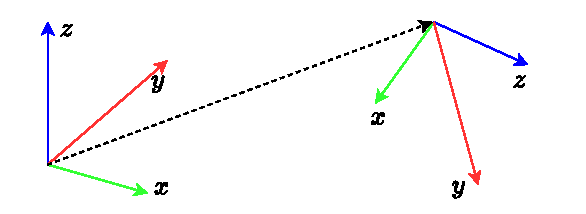
\includegraphics[width=0.7 \textwidth]{Homogeneous Transformation Matrix}
 	\caption[齐次变换矩阵]{齐次变换矩阵} % 中括号中内容为插图索引中显示内容,可在题注内容过长时使用
 	\label{fig:Homogeneous Transformation Matrix}
 \end{figure}
 
齐次变换矩阵是机器人学中广泛应用的一种表示方式,它将一个$3\times3$的旋转矩阵$R$和一个$3\times1$的平移向量$P$结合成一个$4\times4$变换矩阵$T$,如下所示:
\begin{equation}
	\label{equ:Homogeneous Transformation Matrix}
	T=
	\begin{bmatrix}
		R & P \\
		0 & 1 \\
	\end{bmatrix}=
	\begin{bmatrix}
		r_{11} & r_{12} & r_{13} & p_{1} \\
		r_{21} & r_{22} & r_{23} & p_{2} \\
		r_{31} & r_{32} & r_{33} & p_{3} \\
		0 & 0 & 0 & 1 \\
	\end{bmatrix}
\end{equation}
这种表示方法可以在统一框架中高效地组合和处理位姿,如\cref{fig:Homogeneous Transformation Matrix}所示。

 \subsubsection*{(2)欧拉角和四元数}
 
 \begin{figure}[htb]
 	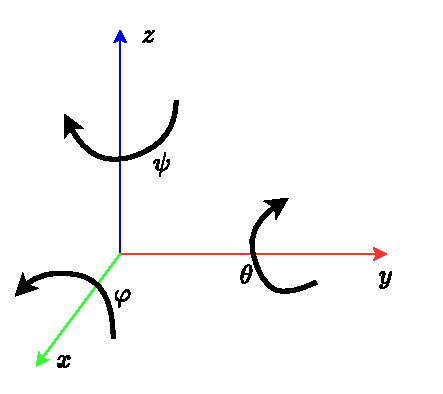
\includegraphics[width=0.43 \textwidth]{olErger.drawio}
 	\caption[欧拉角]{欧拉角} % 中括号中内容为插图索引中显示内容,可在题注内容过长时使用
 	\label{fig: olErger.drawio}
 \end{figure}
 
另一种表示姿态的方法是欧拉角,它引入了三个角度$(\phi,\theta,\psi)$,通过绕主要坐标轴的三次连续旋转来定义物体的朝向,如\cref{fig: olErger.drawio}所示,旋转矩阵$M$可以表示为三个旋转矩阵的乘积:
\begin{equation}
	\label{equ:oulEqu_1}
	M =R_{yz}(\phi)R_{zx}(\theta)R_{xy}(\psi) \\
\end{equation}
\begin{equation}
	\label{equ:oulEqu_2}
	M =
	\begin{bmatrix}
		1 & 0& 0  \\
		0 & \cos\phi & -\sin\phi \\
		0 & \sin\phi & \cos\phi  \\
	\end{bmatrix}
	\begin{bmatrix}
		\cos\theta & 0& \sin\theta  \\
		0 & 1 & 0 \\
		-\sin\theta & 0 & \cos\theta  \\
	\end{bmatrix}
	\begin{bmatrix}
		\cos\psi & -\sin\psi& 0  \\
		\sin\psi & \cos\psi & 0 \\
		0 & 0 & 1  \\
	\end{bmatrix}
\end{equation}

尽管欧拉角具有直观的优势,但它存在万向节锁死问题,即在某些情况下失去一个自由度,导致奇异性,因此不适用于连续运动应用。为了解决这一问题,四元数提供了一种更加稳定且简洁的表示方式,使用四个参数描述旋转,不会发生奇异性。它由一个标量和一个三维向量组成,表示如下:
\begin{equation}
	\label{equ:Quaternion}
	q=(w,x,y,z)
\end{equation}

$w$是标量部分,表示旋转的余弦分量,$(x,y,z)$是向量部分,表示旋转轴的正弦分量。四元数在实时应用中尤其具有优势,因为它们具有较高的计算效率和数值稳定性。

 \subsubsection*{(3)旋转向量}
 
  \begin{figure}[htbp]
 	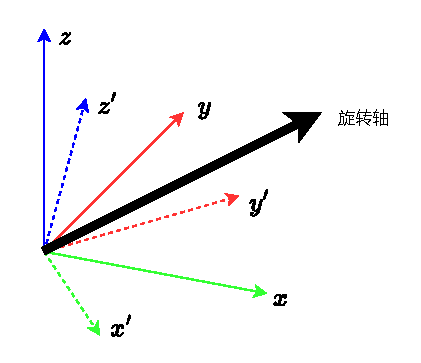
\includegraphics[width=0.43 \textwidth]{rotationVector.drawio}
 	\caption[旋转向量]{旋转向量} % 中括号中内容为插图索引中显示内容,可在题注内容过长时使用
 	\label{fig: rotationVector.drawio}
 \end{figure}
还有一种较为简洁的表示方式是旋转向量(轴-角表示),旋转向量$r$由旋转轴$v$和旋转角度$\theta$组成,定义如下:
\begin{equation}
	\label{equ:rotationVector}
	r=\theta v=(\theta v_{x},\theta v_{y},\theta v_{z})
\end{equation}

其中$v=(v_{x},v_{y},v_{z})$是旋转轴,它是一个单位向量,$\theta$ 是绕该轴旋转的角度,$r$ 是旋转向量,其方向是旋转轴,长度是旋转角度。这种表示方式通常用于优化问题中,当需要简洁但富有表达力的旋转描述时非常有用,如\cref{fig: rotationVector.drawio}所示,原坐标系$O_{xyz}$绕旋转轴旋转变换成坐标系$O_{x^{\prime}y^{\prime}z^{\prime}}$。


\subsection{坐标系与变换}
 \begin{figure}[htb]
	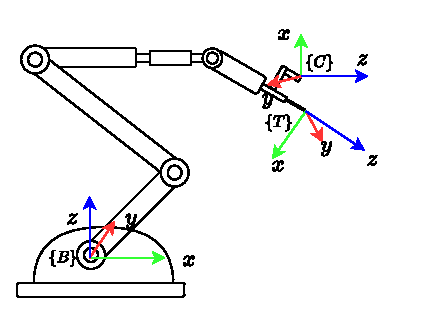
\includegraphics[width=0.6 \textwidth]{translation.drawio}
	\caption[机械臂中各个坐标系]{机械臂中各个坐标系} % 中括号中内容为插图索引中显示内容,可在题注内容过长时使用
	\label{fig:translation.drawio}
\end{figure}

在机器人视觉系统中,多个坐标系的精确变换至关重要,包括机器人基座坐标系(Base, \{B\})、末端TCP坐标系(Tool Center Point, TCP, \{T\})、相机坐标系(Camera, \{C\}),以及世界坐标系(World, \{W\}),如\cref{fig:translation.drawio}所示。这些坐标系之间的相互转换是保证机器人精准感知环境、执行任务的关键因素。特别是在动态任务中,坐标精度的误差可能直接影响机器人操作的成功率。因此,采用合理的运动学建模和手眼标定技术,建立精确的坐标转换关系,对于提升机器人系统的操作精度和稳定性具有重要意义。

\subsubsection*{(1)机械臂基座坐标系 }
机器人基座坐标系 \{B\} 作为整个机械臂系统的全局参考系,其原点通常位于机械臂的底座中心,$Z$轴垂直向上,$X$轴沿机械臂初始运动方向。所有关节和末端执行器的位置均相对于该坐标系进行定义。
\subsubsection*{(2)末端TCP 坐标系  }
TCP 坐标系\{T\} 由末端执行器(如夹爪)的工作点决定,通常不与机械臂法兰坐标系重合,而是存在一定的偏移量。其位置和姿态由机器人运动学方程(基于 Denavit-Hartenberg, DH 参数法)计算得出,即:
\begin{equation}
	\label{equ:coordinate_b_t}
	T^{B}_{T}=T^{B}_{J} \cdot T^{J}_{T} 
\end{equation}

其中,$T^{B}_{T} $为基座到机械臂关节的变换矩阵,$JT^{J}_{T}$为机械臂末端的工具偏移矩阵。通过该变换,可以从基座坐标系计算出 TCP 的位姿。
\subsubsection*{(3)相机坐标系 }
相机坐标系\{C\}由安装在机械臂上的视觉传感器(如RGB-D相机)定义,其原点位于相机光心,Z 轴朝向相机视线方向,X 轴向右,Y 轴向下。为了使相机与末端执行器协同工作,必须进行手眼标定(Hand-Eye Calibration),以求得相机与 TCP 之间的空间变换矩阵$T^{T}_{C}$。

\subsubsection*{(4)世界坐标系 }
在许多视觉任务中,机器人需要将检测到的目标点从相机坐标系 $\{C\}$ 映射到世界坐标系 $\{W\}$,这通常通过外部标定方法(如 AprilTag 或棋盘标定)获得变换矩阵 $T^{W}_{C}$。最终,目标点的世界坐标可以通过以下公式计算:
\begin{equation}
	\label{equ:coordinate_w_c}
	P_{W}=T^{W}_{C} \cdot P_{C} 
\end{equation}

其中,$P_{C} $为相机坐标系中的目标点,$P_{W}$为世界坐标系中的目标点。

\subsubsection*{(5)机械臂多坐标系转换的数学描述 }
2. 机械臂多坐标系转换的数学描述
各坐标系之间的变换通常采用齐次变换矩阵(Homogeneous Transformation Matrix),其形式为:
\begin{equation}
	\label{equ:coordinate_base}
	T^{A}_{B} =
	\begin{bmatrix}
		R_{3 \times 3} & t_{3\times 1}  \\
		0_{1 \times 3} & 1\\
	\end{bmatrix}
\end{equation}


其中$R_{3 \times 3}$为3$\times$3旋转矩阵,描述坐标系的方向变换; $t_{3 \times 1}$为3$\times$1平移向量,描述坐标系的位移变换。综合考虑所有坐标系的变换关系,目标点在基座坐标系中的表示可通过如下公式计算:

\begin{equation}
	\label{equ:coordinate_base_2}
	P_{B} = T^{B}_{T} \cdot T^{T}_{C} \cdot P_{C}
\end{equation}

这表明,若相机检测到某目标点$P_{C}$,可通过末端的手眼标定矩阵$T^{T}_{C}$以及机械臂运动学矩阵$T^{B}_{T}$进行转换,从而得到该目标点在基座坐标系中的位置。


\subsection{物体姿态估计技术}
\subsubsection{基于特征的姿态估计}
基于特征的物体姿态估计方法专注于检测和匹配图像中的显著特征。这些特征作为地标,帮助识别和定位三维空间中的物体。这些经典方法通常用于2D到3D的姿态估计任务,其中通过图像关键点与3D模型点的特征匹配来计算物体在相机坐标系中的姿态。

 \subsubsection*{(1)尺度不变特征变换}
尺度不变特征变换(SIFT) 在三维物体位姿估计任务中,SIFT算法通常用于从单张或多张二维图像中提取稳定的特征点,然后通过匹配这些特征点来推测物体在三维空间中的位置和朝向。

首先,通过从不同视角下拍摄的二维图像中提取SIFT特征点,算法能够在图像中找到具有显著差异和鲁棒性的局部特征。对于每个关键点,SIFT算法会生成一个包含局部图像梯度信息的描述符,确保在光照、旋转、尺度变化等变换下依然能准确地匹配相同的特征点。然后,使用这些匹配的特征点,结合相机的内外参(如相机的焦距和位置),通过几何计算方法(例如PNP算法)来估计物体的位姿。

在实际应用中,SIFT常与其他算法如PNP(Perspective-n-Point)和RANSAC结合使用,以增强位姿估计的准确性和鲁棒性。PNP算法用于通过一组已知3D点与其对应的2D投影点来估计相机的位置和朝向,而RANSAC则用于在特征匹配过程中剔除错误匹配点,从而提升结果的稳定性和准确性。

SIFT在三维物体位姿估计中的一个典型应用是增强现实(AR)。在增强现实应用中,SIFT被用来实时追踪物体的位置和姿态,并将虚拟信息叠加到实际场景中。这要求对物体的三维模型有准确的先验信息,并通过特征匹配来持续调整位姿估计,以确保虚拟物体能够正确地与现实世界中的物体对齐。

此外,SIFT也被广泛应用于3D重建任务中。在多视角的图像中提取到的特征点可以用于通过三角测量计算三维点的空间位置,进而重建出三维物体或场景。该过程中的特征匹配是实现精确重建的关键步骤,而SIFT提供了在不同视角下稳定且独特的特征描述符,极大地提高了匹配的成功率。
 \subsubsection*{(2)加速稳健特征}
SURF(加速稳健特征,Speeded-Up Robust Features) 是一种用于图像特征检测与描述的算法,旨在提高SIFT算法的计算效率,同时保持其稳健性。SURF算法由Bay等人于2006年提出,并在多个计算机视觉任务中广泛应用,如图像匹配、目标识别、三维重建和图像拼接等。与SIFT类似,SURF能够有效地检测到尺度、旋转和光照变化下稳定的特征点,但通过改进计算方法,显著提高了速度。

SURF的核心改进之一是采用Hessian矩阵来进行尺度空间中的特征点检测。通过近似计算Hessian矩阵,Hessian矩阵的形式如下:
\begin{equation}
	\label{equ:Hessian}
	H(x,\sigma) =
	\begin{bmatrix}
		D_{xx}(x,\sigma) & D_{xy}(x,\sigma)  \\
		D_{xy}(x,\sigma)  & D_{yy}(x,\sigma) \\
	\end{bmatrix}
\end{equation}

其中$D_{xx}(x,\sigma)$ ,$D_{xy}(x,\sigma)$ ,$D_{yy}(x,\sigma)$ 是图像的二阶偏导数,表示图像在各方向的曲率。Hessian矩阵的特征值能够反映图像中局部区域的强度变化,从而识别出重要的特征点。

SURF能够在不同尺度下快速检测到图像中的显著特征点。此外,SURF通过引入积分图的加速技术,使得图像梯度的计算更加高效,从而降低了计算复杂度,相较于SIFT在处理速度上具有显著优势。

为了实现旋转不变性,SURF为每个特征点分配一个主方向,该方向基于关键点邻域内的梯度方向进行计算。SURF的特征描述符基于Haar小波响应,通过计算关键点邻域内的局部梯度来生成描述符。这些描述符能够高效地描述图像的局部结构,并且在光照、旋转和尺度变化下保持不变性。

SURF在计算效率上优于SIFT,是一个在许多计算机视觉任务中广泛应用的强大工具,尤其是在需要快速特征提取和匹配的场景中,如全景拼接、实时物体追踪和三维重建等。
 \subsubsection*{(3)Oriented FAST and Rotated BRIEF}
ORB(Oriented FAST and Rotated BRIEF)是一种结合了FAST角点检测和BRIEF描述符的特征点检测与描述算法,主要用于计算机视觉中的特征匹配和图像配准。它由Ethan Rublee等人于2011年提出,旨在提高传统方法在旋转不变性和计算效率上的性能。ORB不仅具备较高的鲁棒性,还能在实时应用中保持较快的运行速度,因此被广泛应用于诸如物体识别、图像拼接和机器人定位等领域。

ORB的核心思想是首先使用FAST(Features from Accelerated Segment Test)角点检测器来检测图像中的角点。FAST是一个高效的角点检测方法,通过分析像素点周围区域的亮度变化来确定角点的存在。与传统的Harris角点检测器相比,FAST具有更快的计算速度,适合于实时处理。但仅使用FAST检测到的角点并不足以解决旋转和尺度变化的问题,因此ORB引入了对角点的方向性分析,以实现对旋转变化的鲁棒性。

为了进一步提高描述符的质量和匹配的准确性,ORB采用了BRIEF(Binary Robust Independent Elementary Features)描述符。BRIEF通过比较特征点邻域内像素对的亮度值来生成二进制字符串,用以描述特征点周围的局部图像信息。这使得描述符具有非常高的计算效率,并且容易存储。然而,BRIEF本身对旋转不具备鲁棒性,因此ORB在生成BRIEF描述符之前,会先为每个角点计算一个主方向,使得生成的描述符在旋转后的图像中仍能保持一致。

尽管ORB并不像SIFT或SURF那样直接支持尺度不变性,但通过图像金字塔结构,ORB可以在不同尺度下检测和描述特征点,从而实现一定程度的尺度不变性。这使得ORB在处理图像中的尺度变化时仍然能够保持较好的表现。此外,ORB具有较强的抗噪声能力,能够在低质量或含有噪声的图像中进行有效的特征匹配和追踪。

\subsubsection{基于深度学习的方法}
与传统方法不同,基于深度学习的方法利用大规模数据集和卷积神经网络(CNN)直接从原始图像数据中估算物体姿态,从而省略了显式的特征提取。这些方法能够有效处理复杂场景,包括遮挡和视角变化,传统方法可能无法应对这些情况。以下是一些在物体姿态估计中突出的深度学习方法:
 \subsubsection*{(1)PoseNet}
 \begin{figure}[htb]
 	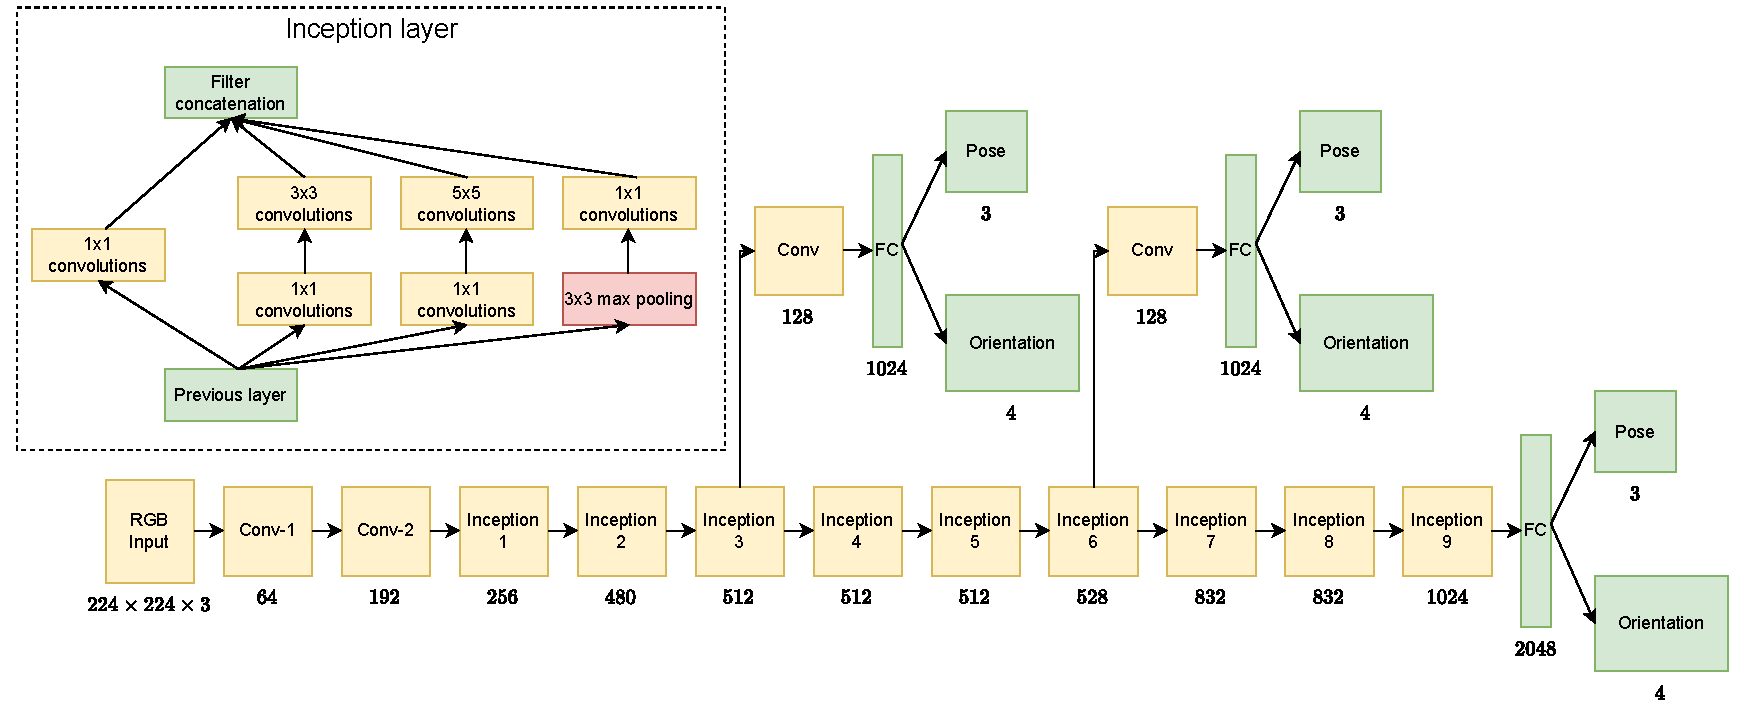
\includegraphics[width=1 \textwidth]{posenet.drawio}
 	\caption[PoseNet模型结构]{PoseNet模型结构} % 中括号中内容为插图索引中显示内容,可在题注内容过长时使用
 	\label{fig:posenet.drawio}
 \end{figure}
 
PoseNet是一种基于深度学习的方法,通过卷积神经网络(CNNs)直接从单个RGB图像预测6自由度(6-DoF)的相机位姿。这种方法无需显式特征匹配,提高了对环境变化的鲁棒性,并能推广到不同的场景。与依赖人工特征提取的方法不同,PoseNet通过监督学习直接从图像像素学习到相机位姿的映射关系。
PoseNet的核心方法涉及训练一个CNN,通常基于GoogleNet或ResNet等架构,以预测相机位姿。该网络由卷积层组成,用于特征提取,随后是全连接层,用于回归相机的6D位姿向量。该向量包括三个空间坐标和四元数表示的方向,从而可以从单张图像中实现稳健的位姿估计。如\cref{fig:posenet.drawio}所示。

在训练过程中,PoseNet用了一个同时平衡位置和方向误差的损失函数。损失函数定义如下:
\begin{equation}
	\label{equ:poseNet}
	L = || x - \hat{x} ||_{2} + \beta||q - \hat{q}||_{2}
\end{equation}

其中, $x$和$q$分别是真实位置和方向,而$\hat{x}$和$\hat{q}$是预测值。权重超参数$\beta$引入,以平衡平移误差和旋转误差的影响,从而确保稳定和准确的位姿预测。

这种方法使PoseNet即使在传统方法因遮挡或缺乏显著特征而失效的情况下仍能有效工作。通过利用CNN,PoseNet能够从图像中提取稳健的特征表示,从而在复杂环境中实现可靠的位姿估计。

 \subsubsection*{(2)DenseFusion}
  \begin{figure}[htb]
 	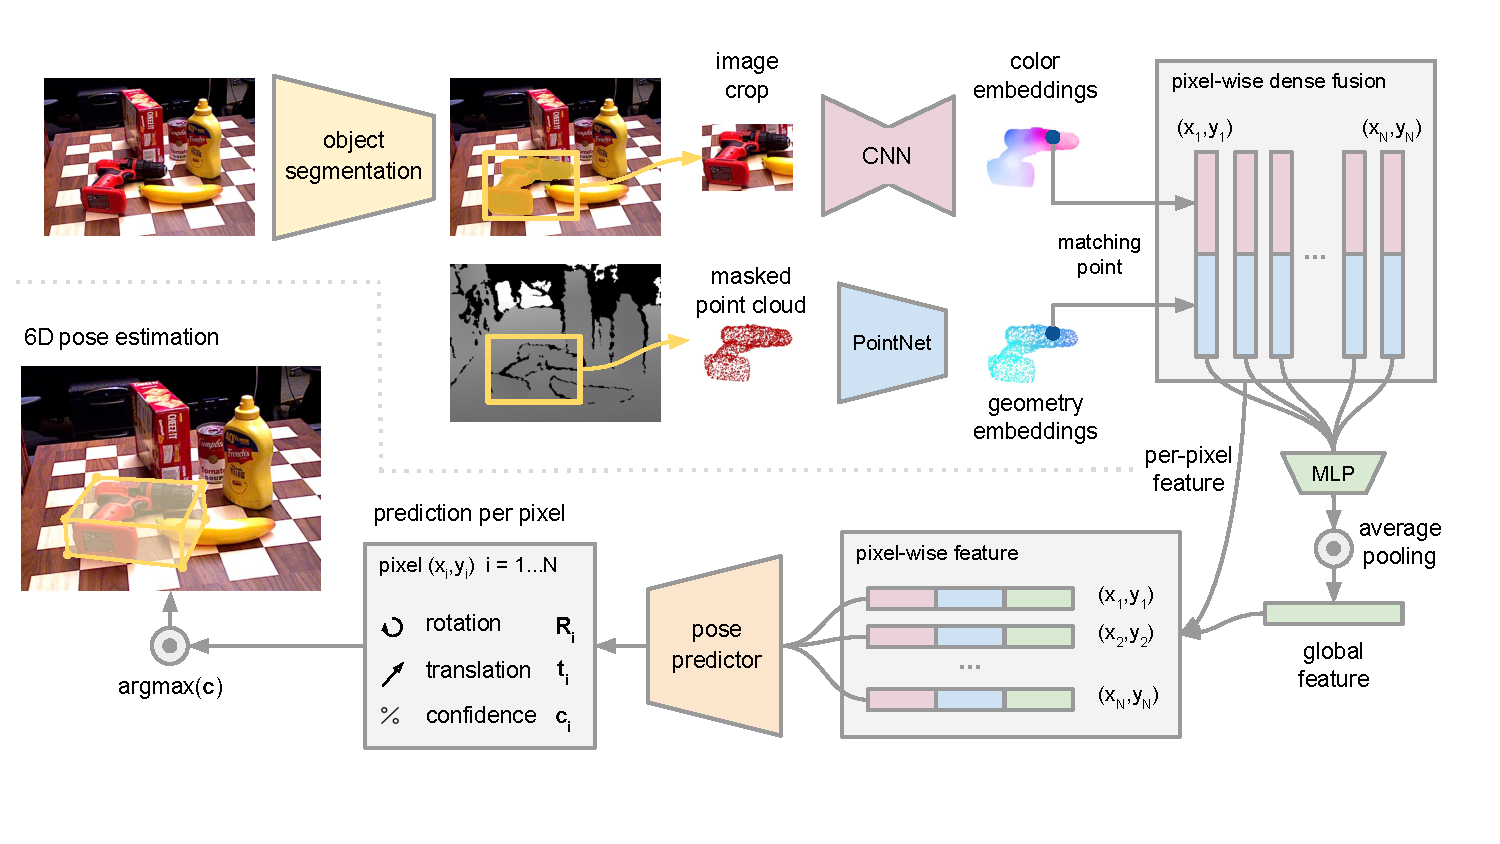
\includegraphics[width=1 \textwidth]{denseFusionoverall_workflow}
 	\caption[DenseFusion工作流程图]{DenseFusion工作流程图} % 中括号中内容为插图索引中显示内容,可在题注内容过长时使用
 	\label{fig:denseFusionoverall_workflow}
 \end{figure}
 
DenseFusion 是一种基于深度学习的 6D 物体位姿估计框架,利用 RGB 和深度(RGB-D)数据 实现精准而鲁棒的位姿预测。不同于依赖手工特征的传统方法,DenseFusion 采用 像素级特征融合,分别提取 RGB 和深度特征,然后在每个像素级别进行融合,形成密集的特征表示。这种方法能够同时捕获外观信息和几何信息,使得网络在 遮挡和复杂环境 下依然能够保持较高的估计精度。

DenseFusion 的网络由 特征提取、位姿估计和位姿优化 三个关键阶段组成。首先,CNN 主干网络(如 ResNet) 提取 RGB 特征,而 基于 PointNet 的网络 处理来自 3D 点云的 深度信息。这些特征随后在像素级别进行融合,确保每个像素都携带丰富的视觉和空间数据。融合后的特征通过 多层感知机(MLP) 进行处理,直接预测物体的 6D 位姿(旋转 + 平移)。然而,由于初始预测可能存在误差,DenseFusion 还包含一个 位姿优化模块,该模块通过最小化预测位姿与观测深度数据之间的差异,迭代优化位姿估计,显著提高最终的估计精度,工作流程如\cref{fig:denseFusionoverall_workflow}所示。

DenseFusion 的损失函数用来最小化3D模型上的采样点在真实位姿下的坐标与在预测位姿下的坐标之间的欧氏距离的均值。并且针对非对称和对称物体选取了不同的损失函数,其中非对称物体的损失函数为:
\begin{equation}
	\label{equ:denseFusion_1}
	L^{p}_{i} = \frac{1}{M}\sum\limits_{j}||(Rx_{j} +t)-(\hat{R}_{i}x_{j} + \hat{t}_{i})||
\end{equation}

其中,$x_{j}$表示从物体三维模型中随机选取的M个三维点中的第 j 个点,$R$和$t$是真实姿态,$\hat{R}_{i}$和$\hat{t}_{i}$是根据第 i 个密集像素的融合嵌入生成的预测姿态。

对称物体的损失函数为:
\begin{equation}
	\label{equ:denseFusion_2}
	L^{p}_{i} = \frac{1}{M}\sum\limits_{j}\min\limits_{0<k<m}||(Rx_{j} +t)-(\hat{R}_{i}x_{j} + \hat{t}_{i})||
\end{equation}

对所有预测的每个高密度像素的姿态进行优化,就是最小化每个高密度像素损失的平均值,用密集像素置信度对每个密集像素的损失进行加权,并添加第二个置信度正则化项,最终的损失函数为:
\begin{equation}
	\label{equ:denseFusion_3}
	L= \frac{1}{N}\sum\limits_{i}(L_{i}^{p}c_{i} - w\log(c_{i}))
\end{equation}

其中,$N$为从片段的$P$个元素中随机采样的密集像素特征的数量,$w$为平衡超参数。
\subsubsection*{(3)PVNet}
  \begin{figure}[htb]
	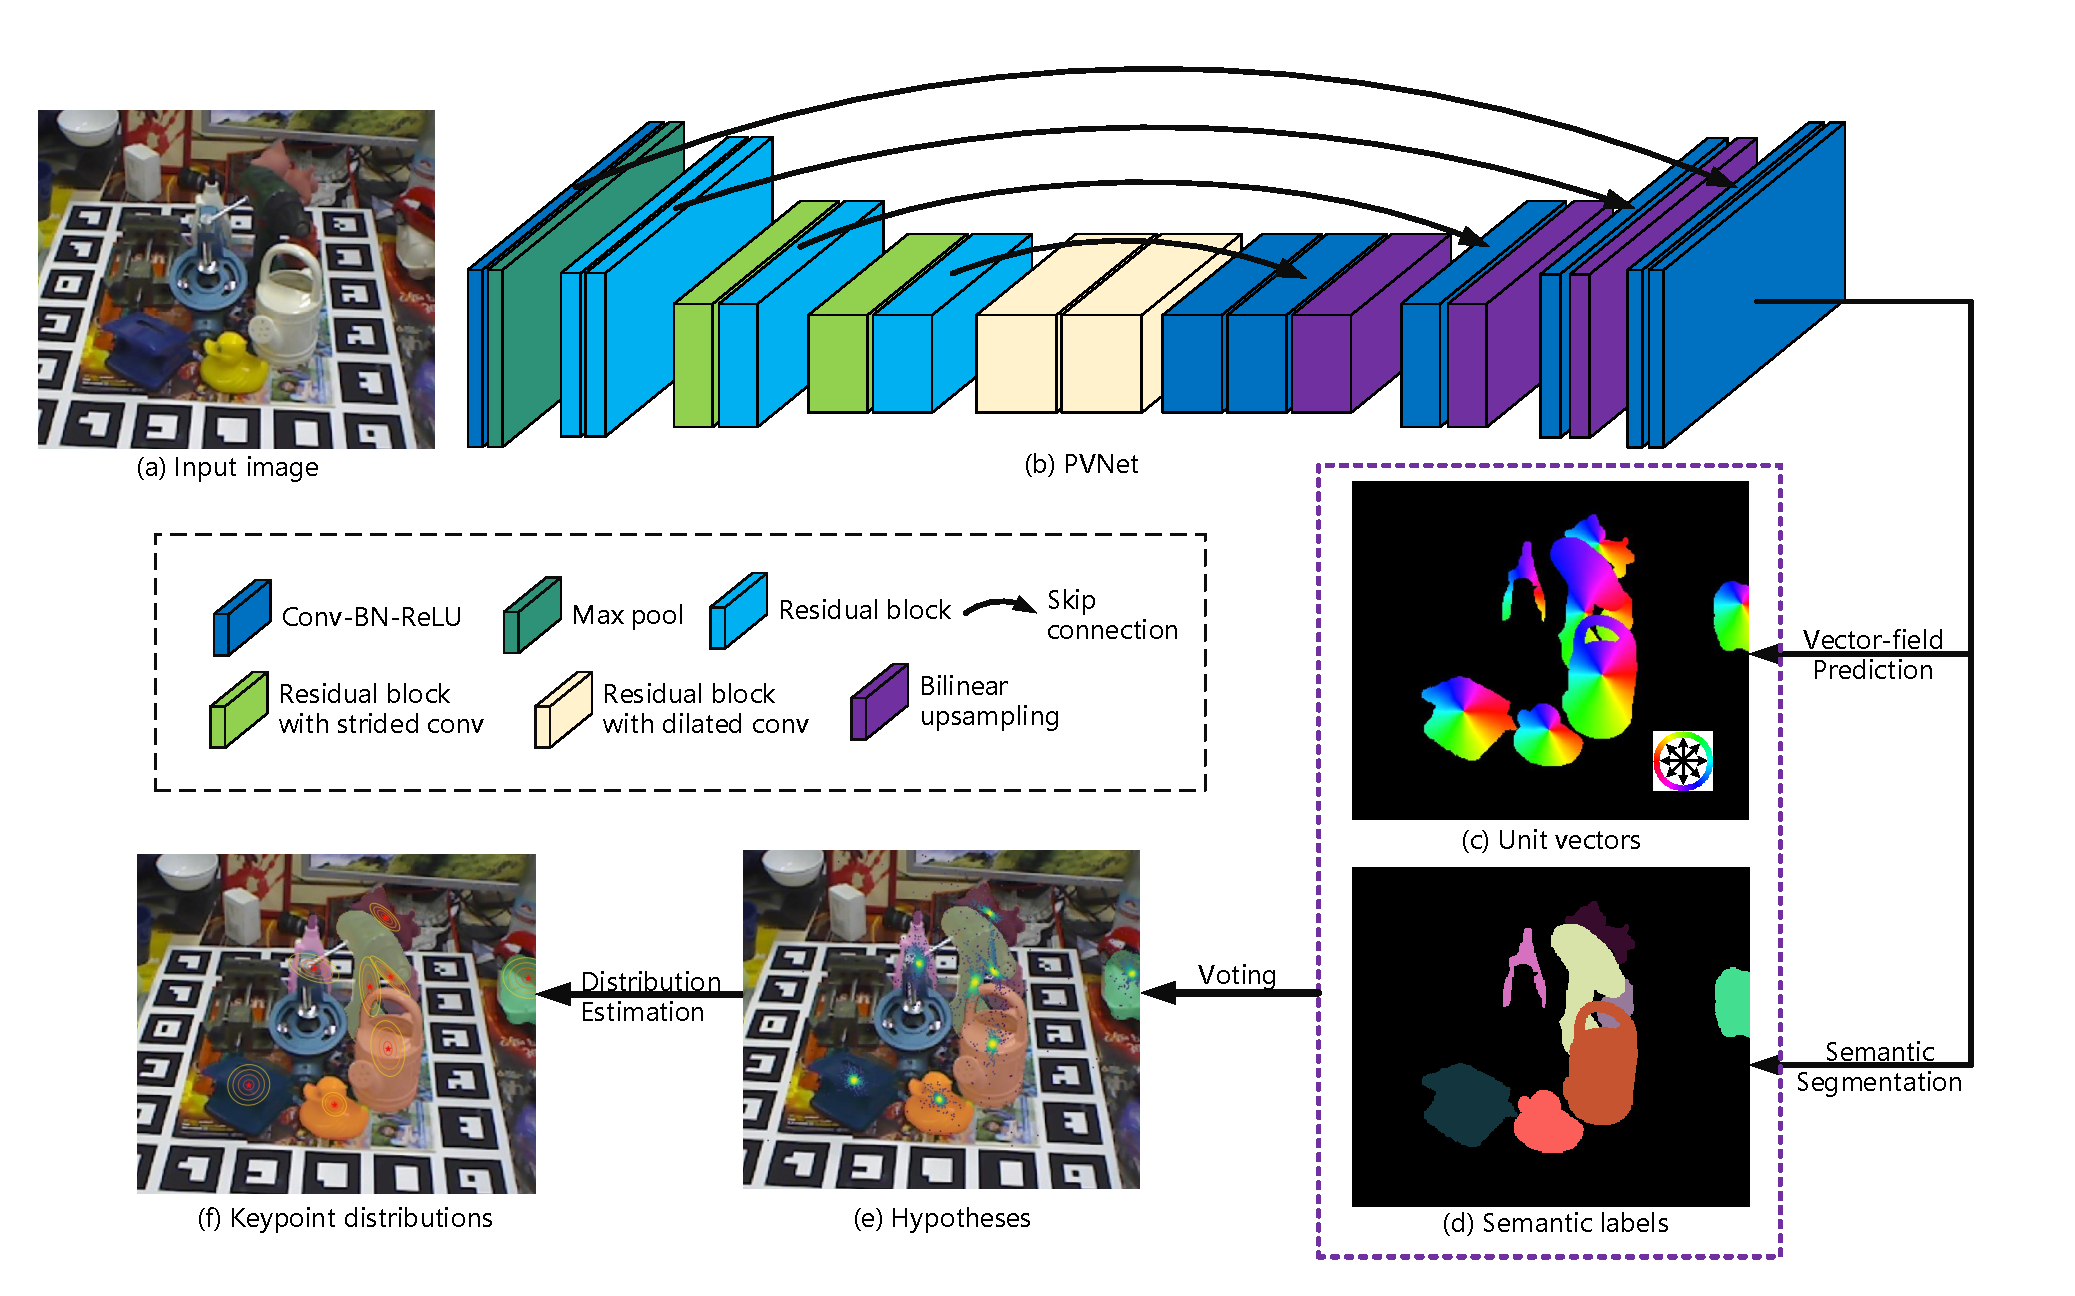
\includegraphics[width=1 \textwidth]{pvnet}
	\caption[关键点定位概述]{关键点定位概述: (a) Occlusion LINEMOD 数据集图像。(b) PVNet 的架构。(c)
		指向物体关键点的像素矢量。(d) 语义标签。(e) 通过投票产生的关键点位置假设。投票得分较高的
		投票得分越高的假设越亮。(f) 根据假设估算出的关键点位置的概率分布。分布的
		分布的平均值用红星表示,协方差矩阵用椭圆表示。} % 中括号中内容为插图索引中显示内容,可在题注内容过长时使用
	\label{fig:pvnet}
\end{figure}
PVNet(姿态与视角网络)是一种基于深度学习的6D物体姿态估计方法,旨在从单张RGB图像中估计物体的位置信息(平移)和方向信息(旋转)。与传统方法不同,PVNet能够有效应对视角变化和部分遮挡问题,这使得它在现实场景中表现尤为出色,尤其是当物体可能部分被遮挡或以非标准角度被观察时。它能够在这些具有挑战性的条件下准确估计物体的姿态,远优于早期在泛化能力方面表现较差的技术。

PVNet的核心使用卷积神经网络(CNN)从输入图像中提取高层次特征,然后预测物体上的关键点。这些关键点对于确定物体的姿态至关重要。通过将这些关键点与物体的3D模型进行匹配,网络能够计算出物体的6D姿态(平移和旋转)。此外,PVNet还能够估计物体的视角,从而进一步提高估计精度,能够有效应对不同的观察角度和姿态变化。\cref{fig:pvnet}展示了PVNet工作流程概述。

PVNet的一大优势是它对遮挡的鲁棒性。在许多现实应用中,物体往往会被部分遮挡,这使得传统的姿态估计方法难以应对。通过聚焦于物体的关键点,即使物体的一部分不可见,PVNet依然能够生成准确的姿态估计。这一特性使得它在机器人领域尤其有用,因为在机器人操作中,物体并不总是完全可见的。

PVNet是一个端到端的深度学习框架,这意味着它能够直接从原始图像中学习,无需手动进行特征工程。这简化了PVNet在各种应用中的部署,包括机器人、增强现实(AR)和自动驾驶汽车等领域。


\section{机械臂运动规划}
运动规划是机器人学中的一项关键任务,特别是对于介尺度机械臂,它们被设计用于执行精确和细致的运动。这些机器人臂广泛应用于需要高精度的领域,如精准授粉、外科机器人和微组装等。运动规划的目标是生成一条轨迹,使机器人臂能够从初始位置移动到目标位置,同时避开障碍物并优化运动效率。在环境要求机器人臂必须适应动态条件时,运动规划任务会变得更加复杂,使得适应性成为规划过程的关键因素。
传统的运动规划方法,如插值法,在结构化环境中有效,提供了平滑和高效的路径。然而,随着机器人任务的复杂性增加,特别是在非结构化环境中,新的技术如深度学习逐渐成为有价值的工具。这些方法使机器人臂能够通过从环境反馈和传感数据中学习,自主地调整到新的情境中。本文讨论了基于传统插值法的方法和现代深度学习方法,并强调了每种方法在解决机器人运动规划挑战,特别是精准授粉任务中的贡献。
在执行精密操作时,介尺度机械臂面临几项关键挑战。包括:
1.	精度与准确性:高精度对于执行如花粉传播等细致任务至关重要,因为即便是微小的运动偏差也可能导致失败。机器人臂必须执行高精度的运动,通常需要达到亚毫米级的精度,以避免损坏易碎的物体或组件。
2.	动态环境:机器人臂必须在动态环境中工作,障碍物或物体可能会不可预测地移动,这要求机器人臂实时调整其轨迹。在某些应用中,环境可能还包括变化的光照条件或杂乱的场景,进一步增加了运动规划的难度。
3.	有限的工作空间与障碍物:许多机器人臂在空间有限的环境中操作,必须高效地避免碰撞。路径规划必须考虑到障碍物以及与其他物体或机器人系统的潜在干扰,确保机器人臂在有限的工作空间内安全有效地移动。
当这些因素相互结合时,运动规划的复杂性增加,因此需要结合传统方法与深度学习技术,以达到最佳性能。



\subsection{传统运动规划方法}

在实际应用中,插值方法被广泛用于路径生成和轨迹规划。例如,在精准授粉中,机器人臂需要沿着预定义路径运动,同时避开障碍物并减少对脆弱花朵的影响。通过使用三次或五次样条插值,机器人臂可以生成最小化突然运动的轨迹,确保路径点之间的平稳过渡。
插值方法使机器人能够高效地跟随复杂路径,无论是在关节角度还是末端执行器的位置之间进行插值。在授粉任务中,机器人臂必须从一朵花移动到另一朵花,运动的平滑性至关重要,以避免对花朵造成损害。使用三次和五次样条插值确保机器人可以平稳地从一个位置到另一个位置,调整花朵的朝向等环境变化。
通过生成优化路径,机器人臂可以减少不必要的运动,从而提高任务效率。在精准授粉的背景下,减少运动时间对于提高产量和提升系统性能非常重要。
插值法长期以来一直是机器人臂运动规划的核心技术。它通过计算预定义路径点之间的中间点,生成机器人臂的平滑路径。几种插值方法在实践中被广泛应用:

\subsubsection{线性插值(Lerp)}
 \begin{figure}[htb]
	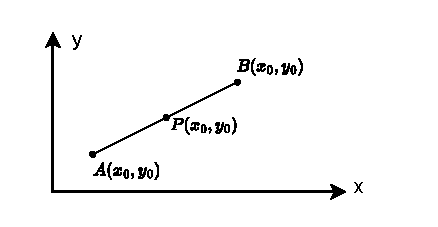
\includegraphics[width=0.5\textwidth]{lerp.drawio}
	\caption[线性插值]{线性插值} % 中括号中内容为插图索引中显示内容,可在题注内容过长时使用
	\label{fig:lerp.drawio}
\end{figure}
线性插值(Linear Interpolation,简称 Lerp)是一种在两个已知数据点之间计算中间值的方法。其基本思想是基于一个插值因子$t$(通常在 0 到 1 之间),按照比例在两个点之间进行平滑过渡,如\cref{fig:lerp.drawio}所示。线性插值广泛应用于计算机图形学、信号处理、运动规划、物理仿真、机器人路径控制等领域。
在机器人运动控制中,Lerp 可用于在已知的起始位置和目标位置之间生成平滑的运动轨迹,以确保运动的连续性和稳定性。

给定两个点$A$和$B$,其坐标分别为$A(x_{0},y_{0})$和$B(x_{1},y_{1})$,线性插值计算一个参数$t(t\in[0,1])$对应的插值点$P(x,y)$:
\begin{equation}
	\label{equ:Lerp:1}
	P=A + t(B-A)
\end{equation}

然而,对于需要平滑过渡的复杂任务,线性插值通常过于简单。例如,当机器人在两个点之间改变朝向时,运动不够平滑。
\subsubsection{球面线性插值(Slerp)} 
 \begin{figure}[htb]
	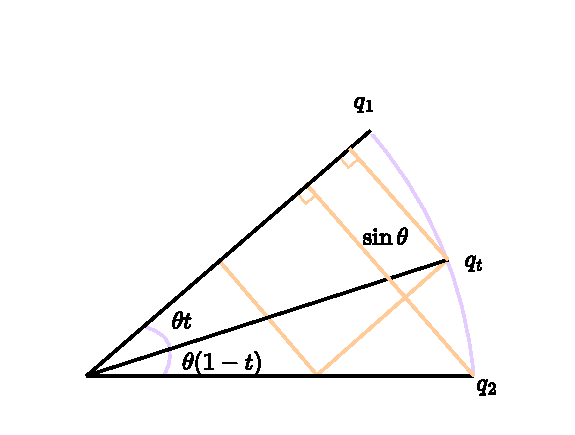
\includegraphics[width=0.6\textwidth]{Slerp.drawio}
	\caption[球面线性插值]{球面线性插值} % 中括号中内容为插图索引中显示内容,可在题注内容过长时使用
	\label{fig:Slerp.drawio}
\end{figure}
球面线性插值(Slerp)是一种用于单位向量或单位四元数之间的平滑插值方法,确保旋转沿着球面最短路径进行。它广泛应用于 3D 计算机图形学、机器人运动控制和动画平滑过渡等场景。Slerp 的核心原理是基于两个旋转状态的夹角,通过三角函数插值计算出中间旋转状态,使得旋转过程保持恒定角速度,从而避免线性插值(Lerp)可能产生的旋转变形问题,如\cref{fig:Slerp.drawio}所示。

Slerp 的计算公式如下:给定两个单位四元数$q_{1}$和$q_{2}$,以及插值因子$t(t\in[0,1])$,插值点$q(t)$可表示为:
\begin{equation}
	\label{equ:Slerp:1}
	Slerp(q_{1},q_{2},t)=\frac{\sin((1-t)\theta)}{\sin(\theta)}q_{1} + \frac{\sin(t\theta)}{\sin(\theta)}q_{2}
\end{equation}

其中,$\theta$是四元数$q_{1}$和$q_{2}$之间的夹角,由点积计算得到:
\begin{equation}
	\label{equ:Slerp:2}
	\cos(\theta)=q_{1} \cdot{q_{2}}
\end{equation}

Slerp 的主要优势在于,它可以沿球面最短路径插值,避免 Lerp 可能造成的旋转失真,并且保持恒定角速度,使得旋转过渡更加自然。
\subsubsection{三次样条插值}  
 \begin{figure}[htb]
	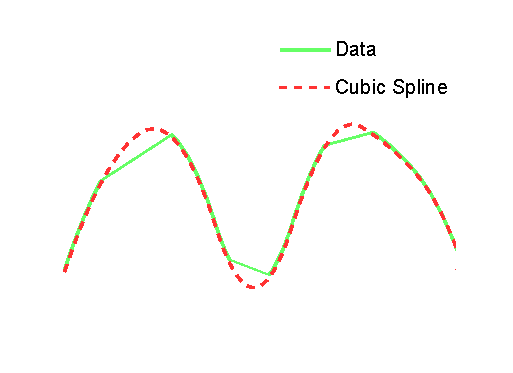
\includegraphics[width=0.5\textwidth]{Cubic Spline Interpolation.drawio}
	\caption[三次样条插值示意图]{三次样条插值示意图} % 中括号中内容为插图索引中显示内容,可在题注内容过长时使用
	\label{fig:Cubic Spline Interpolation.drawio}
\end{figure}
三次样条插值(Cubic Spline Interpolation)是一种用于平滑插值的方法,能够在数据点之间创建连续、光滑的曲线。与高阶多项式插值相比,三次样条插值能够有效避免振荡现象,因此广泛应用于计算机图形学、机器人路径规划、数据拟合和信号处理等领域。其基本思想是使用多个三次多项式函数,在相邻数据点之间进行插值,同时确保整体曲线的光滑性,如\cref{fig:Cubic Spline Interpolation.drawio}所示。

在三次样条插值中,对于一组数据点$(x_{0},y_{0}),(x_{1},y_{1}),(x_{2},y_{2}),...,(x_{n},y_{n})$,系统需要在每两个相邻点之间构造一个三次多项式$S_{i}(x)$来表示曲线段。该多项式的形式为:
\begin{equation}
	\label{equ:Cubic Spline Interpolation 1}
	S_{i}(x) = a_{i} + b_{i}(x-x_{i}) + c_{i}(x-x_{i})^{2} + d_{i}(x-x_{i})^{3}  
\end{equation}

为了确保整体曲线的平滑性,系数$a_{i},b_{i},c_{i},d_{i}$需要满足一系列约束条件。首先,插值曲线必须经过所有数据点,即满足插值条件。其次,在相邻的插值段之间,一阶导数必须连续,以确保曲线的平滑过渡。此外,二阶导数也必须连续,以保持曲率的平滑性。最后,还需要引入适当的边界条件,例如自然边界(两端二阶导数为零)、夹持边界(指定端点的一阶导数)或周期性边界(确保首尾曲线平滑衔接)。这些条件共同构成了一个三对角线性方程组,通过求解该方程组,即可得到每段插值函数的系数。

在具体计算过程中,我们首先计算数据点之间的间隔$h_{i} = x_{i+1} - x_{i}$,然后根据二阶导数的连续性条件构造方程组。解出二阶导数$M_{i}$之后,可以进一步计算各段插值多项式的系数:

\begin{equation}
	\label{equ:Cubic Spline Interpolation 2}
	\begin{split}
		b_{i} &= \frac{y_{i+1} - y_{i}}{h_{i}} - \frac{h_{i}}{6}(M_{i+1} + 2M_{i})   \\
		c_{i} &= \frac{M_{i}}{2} ,d_{i} = \frac{M_{i+1} - M_{i}}{6H_{i}}
	\end{split}
\end{equation}

三次样条插值在多个领域有广泛应用。例如,在机器人路径规划中,它可用于计算平滑的运动轨迹,确保机械臂运动过程中没有突兀的加速或减速变化,从而提高运动的稳定性。在计算机动画中,三次样条能够让角色的运动过渡更加自然,避免生硬的动作切换。此外,在数据拟合和图像处理领域,三次样条插值可用于创建高精度的光滑曲线,适用于信号平滑和图像变形处理。

与其他插值方法相比,三次样条插值的优势在于其高平滑性和稳定性。它能够有效避免拉格朗日插值或高阶多项式插值可能出现的振荡现象,同时提供更加可控的曲线形状。然而,由于需要解一个线性方程组,其计算量比线性插值或分段线性插值略大。


\subsection{深度学习方法}
尽管传统的插值方法在控制环境中有效,但深度学习在解决更复杂的动态运动规划挑战中越来越受到关注。深度学习技术在解决复杂运动规划问题,特别是在动态或非结构化环境中,越来越受到重视。深度学习使机器人臂能够从传感器数据中学习,从而提高其在实时环境中的适应性和决策能力。

\subsubsection{DQN}
 \begin{figure}[htb]
	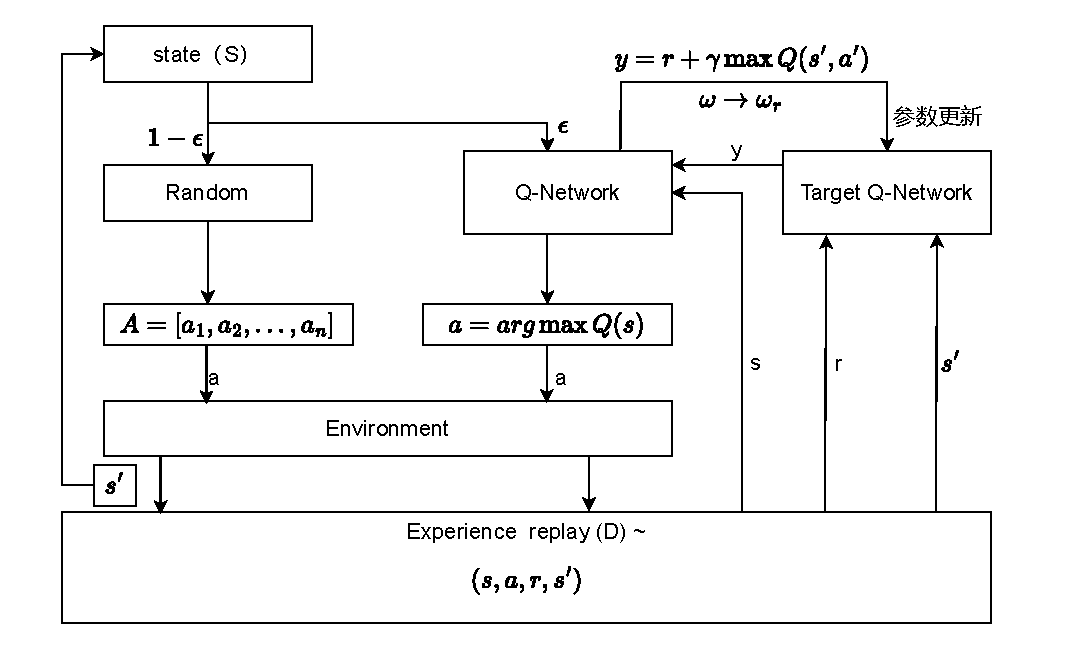
\includegraphics[width=0.85\textwidth]{dqn.drawio}
	\caption[DQN算法流程图]{DQN算法流程图} % 中括号中内容为插图索引中显示内容,可在题注内容过长时使用
	\label{fig:dqn.drawio}
\end{figure}
深度Q网络(Deep Q-Network, DQN)是一种结合深度学习与强化学习的方法,旨在解决高维状态空间下的离散动作决策问题。它最早由 DeepMind 提出。通过CNN处理环境输入,使Q-learning能够适用于复杂任务,如机器人控制、机械臂路径规划、避障和自主抓取等。DQN在Q-learning的基础上引入了深度神经网络,利用 CNN 提取图像特征,从而实现端到端的智能决策。

DQN的核心思想是使用一个深度神经网络$Q(s,a;\theta)$近似$Q$函数,并通过经验回放和目标网络提高训练稳定性。在 Q-learning中,Q值表示机器人在某一状态下执行某一动作的未来累积奖励。DQN通过贝尔曼方程进行Q值更新:
\begin{equation}
	\label{equ:DQN}
	Q(s,a) = r + \gamma\max Q(s^{\prime},a^{\prime})
\end{equation}

其中,$\gamma$是折扣因子,平衡短期与长期奖励。DQN采用CNN 处理高维输入(如图像或点云),再通过全连接层输出各个动作的Q值,最终根据 $\epsilon$-贪心策略选择最优动作,算法流程如\cref{fig:dqn.drawio}所示。

为了提高训练效率和稳定性,DQN 采用了三项关键改进。首先是经验回放(Experience Replay),它通过存储历史经验$(s,a,r,s^{\prime})$并随机采样进行训练,从而打破数据相关性,提高数据利用率。其次是目标网络(Target Network),该方法通过引入一个更新较慢的Q目标网络$Q(s,a,r,s^{\prime})$,防止训练过程中的目标值振荡。此外,DQN 还采用奖励裁剪(Reward Clipping) 来限制奖励范围,避免Q值爆炸。

\subsubsection{DDQN}
双重深度Q网络(Double Deep Q-Network, DDQN)是对 DQN 的改进版本,旨在解决 Q 值过高估计(Q-value Overestimation)的问题,提高强化学习的稳定性和策略优化能力。在 DQN 中,机器人使用Q-learning 进行决策,Q值表示在特定状态下执行某个动作的累积奖励。然而,由于DQN使用同一个网络进行动作选择和Q值评估,容易导致某些动作的Q值被过高估计,进而影响策略收敛。为了解决这一问题,DDQN 通过分离动作选择和Q值计算,降低Q值过高估计的影响,使得机器人在训练过程中更加稳定,并能更精准地选择最优策略。
在 DDQN中,Q值的计算方式进行了关键改进。与DQN直接使用目标网络计算最大Q值不同,DDQN采用两个Q网络:一个是在线Q网络(Online Network),用于选择下一个状态的最优动作;另一个是目标Q网络(Target Network),用于评估这个动作的Q值。在 DDQN中,机器人首先使用在线网络选择最优动作$a^{*}$:
\begin{equation}
	\label{equ:DDQN1}
	a^{*} = arg\max Q_{online}(s^{\prime},a^{*})
\end{equation}
然后使用目标网络评估该动作的Q值:
\begin{equation}
	\label{equ:DDQN2}
	yDDQN = r + \gamma Q_{target}(s^{\prime},a^{*})
\end{equation}
这种方式确保了动作选择和Q值评估分别由不同的网络完成,避免了Q值的过高估计问题,提高了强化学习的可靠性和泛化能力。

在训练过程中,DDQN采用与DQN相似的流程。首先,机器人与环境交互,执行动作并存储经验数据$(s,a,r,s^{\prime})$到经验回放池(Replay Buffer)。然后,从经验池中随机采样数据,计算DDQN的目标Q值,并使用梯度下降更新在线网络的参数。此外,目标网络的参数不会每次训练都更新,而是每隔一定步数才同步,以减少训练震荡,提高学习稳定性。

与 DQN 相比,DDQN主要的优势在于减少了Q值的过高估计问题,提高了机器人的策略质量,同时训练更加稳定,不易出现震荡或收敛到次优解。尽管计算量稍高于DQN,但训练收敛更快,最终策略质量更优。

\subsubsection{LSTM}
传统方法如插值在处理复杂轨迹时,往往容易受噪声影响,并且难以在不同场景下泛化。长短时记忆网络(LSTM)因其出色的时间序列建模能力,能够有效学习运动轨迹的规律,并进行精确的轨迹预测。

LSTM 凭借长时依赖建模能力能够适用于运动轨迹学习。通过输入门、遗忘门和输出门的门控机制,LSTM 可以捕捉轨迹的长时间变化趋势,避免传统循环神经网络(RNN)在长序列任务中遇到的梯度消失问题。此外,LSTM 具有较强的抗噪能力,能够从大量数据中提取轨迹的隐式模式,对环境变化具有较好的适应性。同时,经过充分训练的LSTM具备良好的泛化能力,能够适应不同的轨迹形态,即使遇到未见过的轨迹数据,也能做出较为合理的预测。

在轨迹学习任务中,LSTM 的输入通常是轨迹的历史点序列,包括姿态信息$(x,y,z,rx,ry,rz)$、速度、加速度以及机器人自身的状态信息,如关节角度。输出则是预测的未来轨迹点。为了增强特征提取能力,常采用多层 LSTM 结构,并结合全连接层进行回归预测。训练过程中,均方误差(MSE)常用于轨迹预测任务,而交叉熵损失则适用于轨迹分类。优化器通常选择 Adam 或 RMSprop,以提高收敛速度和稳定性。

 在运动轨迹学习中的应用非常广泛。在机器人运动规划中,它可以用于预测下一步关节运动,提高控制精度。在自动驾驶系统中,它能够预测前方车辆或行人的轨迹,辅助车辆决策。在人类行为预测领域,LSTM 还能学习行人或车辆的运动模式,使机器人能够更自然地与人类交互。






    %% !Mode:: "TeX:UTF-8"
%此为章节二模板
%\chapter、\section、\subsection、\subsubsection分别对应一二三四级标题



    % !Mode:: "TeX:UTF-8"

\chapter{面向花朵位姿检测的目标分割}\label{ch:3}
\iffalse
\section{引言}
在现代农业中,自动化授粉技术正在成为解决劳动力短缺、提高作物产量和品质的重要手段。其中,机械臂柔顺控制的精准授粉任务对环境感知能力提出了极高的要求。要实现高效、稳定的授粉操作,机械臂需要能够准确感知花朵的空间特征,包括位置、形态、朝向等信息。这些信息的准确性直接决定了授粉的成功率和稳定性,因此,位姿检测是精准授粉技术的关键环节。

为了感知环境信息,机器人通常依赖各种传感器,例如RGB摄像头、深度相机、激光雷达等。其中,RGB-D深度相机由于能够同时提供彩色信息和深度信息,且成本较低,成为农业领域常用的视觉传感器。然而,在复杂的温室或田间环境中,由于光照条件的变化、花朵表面反射特性、叶片遮挡等因素,深度相机采集的数据往往存在噪声、空洞、误差等问题,导致位姿检测精度下降。因此,在使用深度相机数据进行位姿估计前,必须对其进行预处理,包括深度数据修正、去噪、补全等,以确保位姿信息的准确性。

此外,为了便于人机交互和授粉轨迹规划,本章提出了一种基于对称空间的花朵位姿检测方法,能够实时构建虚拟空间并同步更新授粉目标花朵的三维位置和朝向信息。该方法可以计算空间中花朵的位姿,为机械臂的授粉任务提供直观、准确的位姿参考信息,并为后续优化机械臂的运动轨迹提供数据。本章方法的整体技术路线主要包括目标分割、深度校正和位姿估计三个部分:首先,使用基于深度学习的实例分割方法对花朵区域进行精确提取;其次,采用深度校正算法对RGB-D相机采集的数据进行优化,以减少噪声并提高深度信息的可靠性;最后,结合三维重建技术,估计花朵的位姿信息。
\fi
\section{引言}

在机械臂执行精准授粉任务的过程中,准确识别花朵的位置和形态是确保授粉成功的关键。然而,在实际的农业场景中,花朵通常处于复杂的背景环境中,容易受到光照变化、遮挡以及花朵自身形态变化的影响,导致分割难度大幅增加。因此,如何高效、准确地分割花朵区域,成为花朵位姿检测中的核心问题。传统的图像处理方法,例如基于颜色分割、边缘检测或形态学处理的手工特征提取方法,虽然在特定条件下能够取得一定的分割效果,但面对不同品种的花朵、复杂的光照环境以及动态变化的遮挡情况,其鲁棒性较差,难以满足自动化授粉系统的要求。

为了克服这些挑战,本章采用基于深度学习的目标分割方法,通过训练神经网络模型,使其能够自动提取花朵的特征并实现高精度分割。在深度学习的发展中,实例分割技术已经成为解决目标分割问题的主流方法,其中 Mask-RCNN 和 YOLACT 作为两种代表性模型,分别适用于高精度分割和高实时性分割的任务。在本章的研究中,我们结合两者的优势,根据不同应用场景选择合适的目标分割方法,以确保花朵分割的准确性和实时性兼顾。

\section{方法}
\subsection{Mask-RCNN}
 \begin{figure}[htb]
	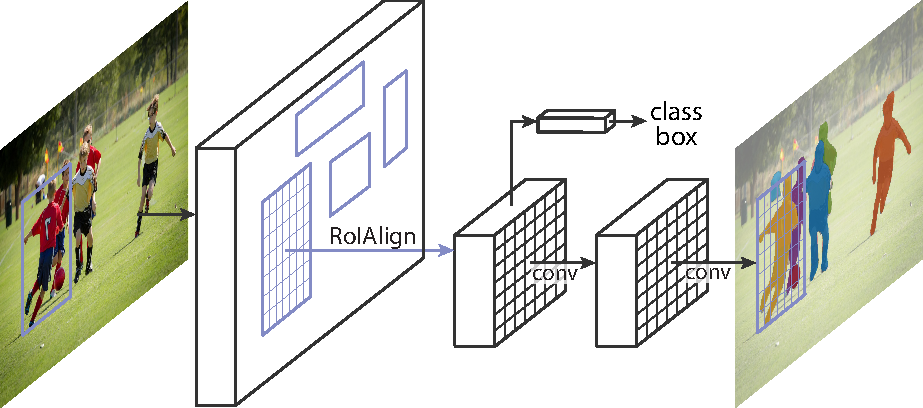
\includegraphics[width=0.6 \textwidth]{mask-rcnn}
	\caption[实例分割Mask-RCNN 框架]{实例分割Mask-RCNN 框架} % 中括号中内容为插图索引中显示内容,可在题注内容过长时使用
	\label{fig:mask-rcnn}
\end{figure}
Mask-RCNN是一种经典的实例分割模型,它是在 Faster-RCNN 目标检测框架的基础上增加了掩膜分割(Mask)分支,使其不仅能够检测目标,还能在像素级别进行分割,如\cref{fig:mask-rcnn}所示。这一特性使得 Mask-RCNN 在花朵检测中具有较高的精度,能够精准地分割出花朵区域,而不受背景影响。在 Mask-RCNN 的模型结构中,首先采用 ResNet-50 或 ResNet-101 作为主干网络,通过卷积神经网络提取图像的高层次特征,并结合特征金字塔网络(FPN, Feature Pyramid Network),增强对不同尺度花朵的检测能力。随后,区域候选网络(RPN, Region Proposal Network)生成候选目标区域,并通过非极大值抑制(NMS, Non-Maximum Suppression)去除冗余的候选框,确保检测的可靠性。最后,ROIAlign 机制用于对目标区域进行精确的特征提取,并通过一个全卷积网络(FCN, Fully Convolutional Network)生成目标的掩膜,实现高精度的实例分割。

Mask-RCNN 在花朵目标分割中的应用表现优异,能够有效应对复杂背景和遮挡问题。然而,由于该模型采用了串行的目标检测和实例分割流程,在计算上开销较大,推理速度相对较慢。在实验环境(NVIDIA GTX 1080 Ti)下,其分割速度约为 5FPS,难以满足实时授粉任务的需求。因此,在实际应用中,若对计算速度要求较高,需要寻找更高效的分割方法,以满足农业机械臂在自动化授粉中的实时性需求。

\subsection{YOLACT}
 \begin{figure}[htb]
	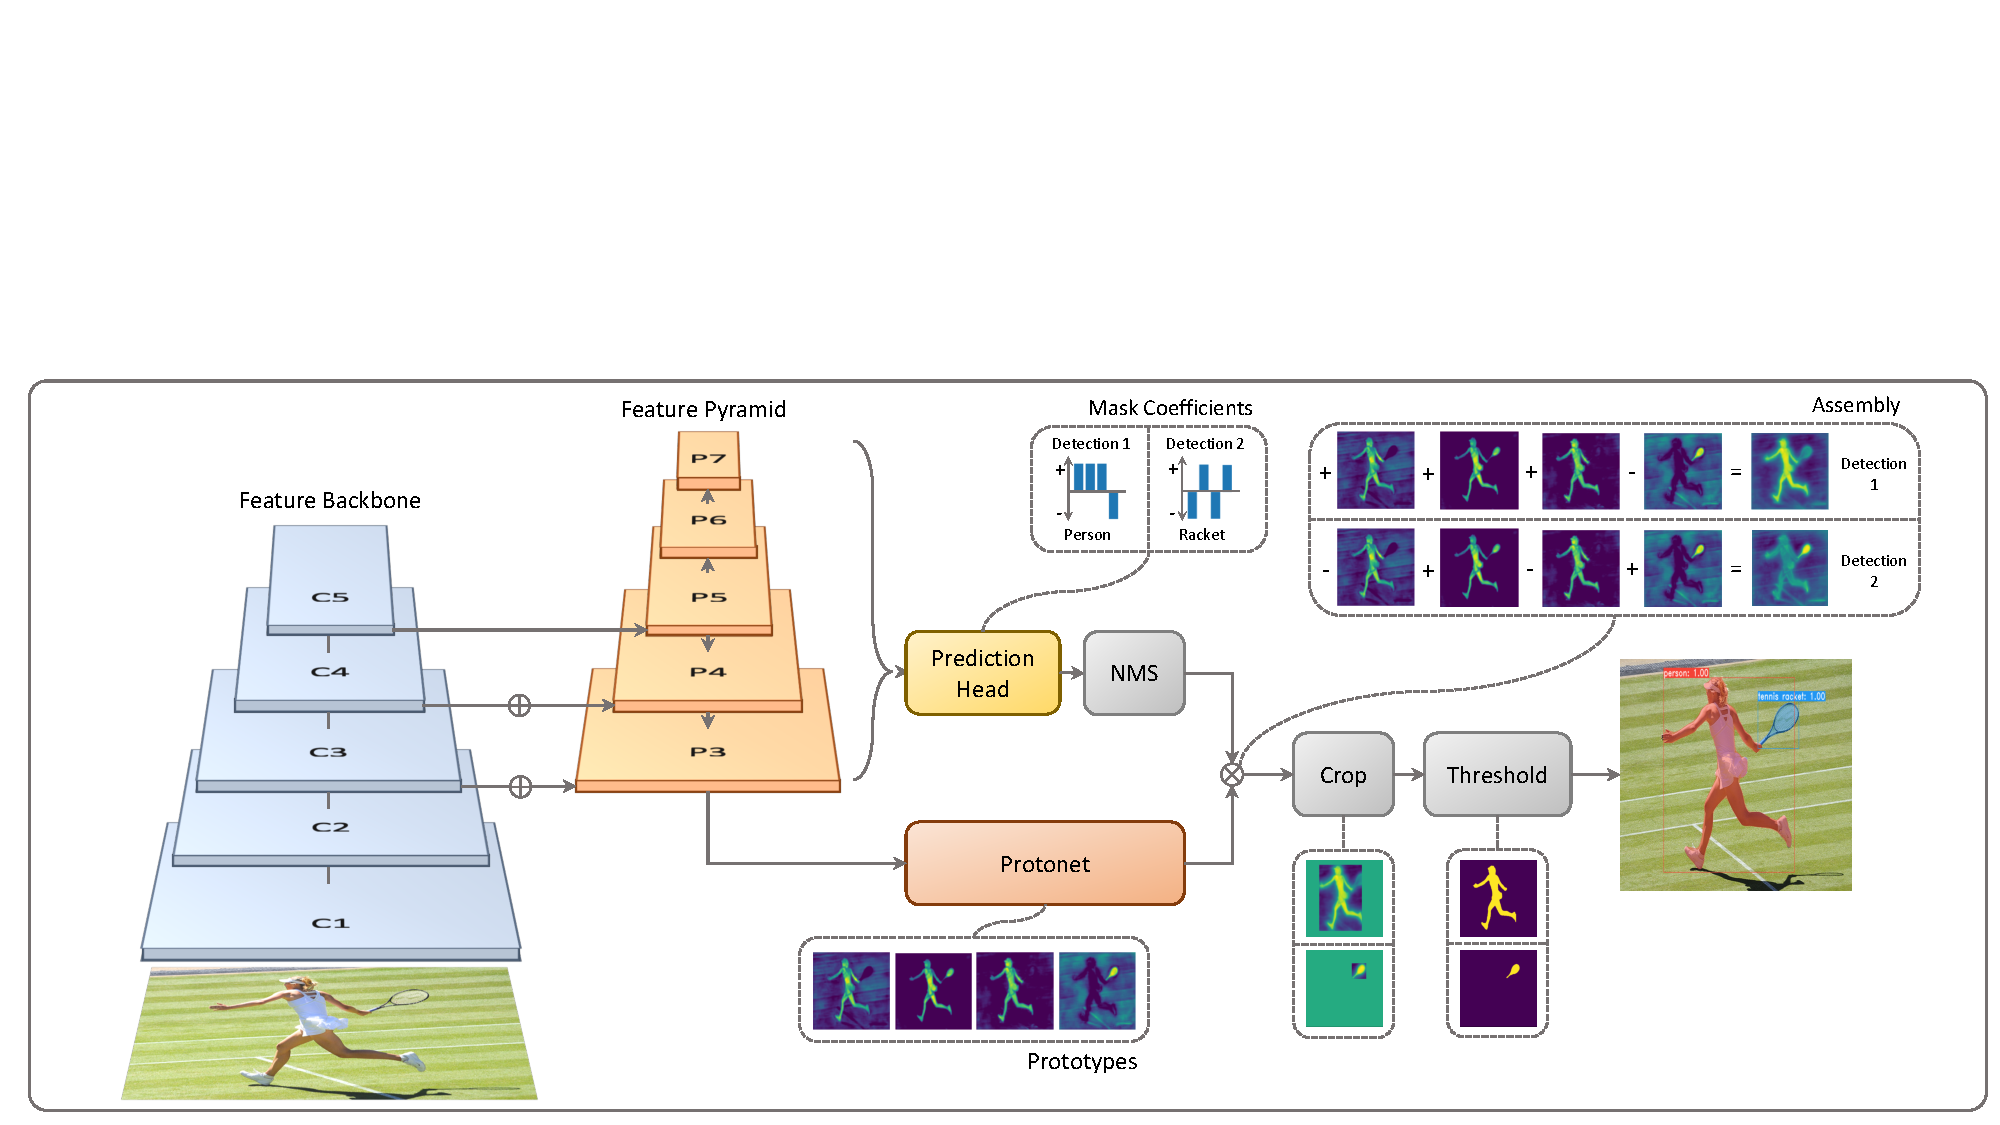
\includegraphics[width=0.8 \textwidth]{yolact}
	\caption[yolact模型架构图]{yolact模型架构图} % 中括号中内容为插图索引中显示内容,可在题注内容过长时使用
	\label{fig:yolact}
\end{figure}
为了解决 Mask-RCNN 在推理速度上的不足,本章引入了 YOLACT(You Only Look At Coefficients, Bolya et al., 2019) 作为优化方案。YOLACT 的核心优势在于 并行执行目标检测和图像分割,避免了 Mask-RCNN 先检测再分割的串行结构,从而大幅提升计算效率。在 YOLACT 的架构中,如\cref{fig:yolact}所示,仍然采用 ResNet-50 或 ResNet-101 作为主干网络,并结合 FPN 提取多尺度特征。在目标检测方面,YOLACT 采用单阶段检测框架,使其可以直接对目标进行分类和定位,而不需要额外的候选区域生成过程。此外,其分割分支通过一个专门的掩膜预测网络,能够在检测的同时进行掩膜预测,使得整个推理过程更加高效。

YOLACT 在授粉任务中的应用主要体现在其优异的实时性。相比于 Mask-RCNN,其计算复杂度大幅降低,在相同实验环境下推理速度可达 34FPS,远高于 Mask-RCNN 的 5FPS。这种高效的计算能力使其更加适用于实时授粉任务,尤其是在需要快速识别和分割花朵,以指导机械臂进行柔顺控制的应用场景。然而,YOLACT 在分割精度上相较于 Mask-RCNN 略有下降,尤其是在边缘处理方面可能存在一定的误差。因此,在高精度需求的场景(如授粉过程中需要确保机械臂末端精准对准花蕊)时,Mask-RCNN 依然是更优的选择,而在需要实时响应的场景(如大规模花卉授粉)中,YOLACT 则更加合适


\section{实验设计与结果分析}
\subsection{实验环境}
本章实验的软硬件设备如表下所示:
\begin{table}[htbp]
	\caption[目标分割实验环境]{目标分割实验环境}
	\setlength{\tabcolsep}{14mm}{ % 因表格过窄,手动设置宽度为7mm
		\begin{tabular}{clc}
			\toprule
			序号    &  设备    & 型号   \\
			\midrule
			1 & realsence相机  & D435i     \\
			2 & cpu  & intelCorei5-13600     \\
			3 & 内存 & 32GB   \\
			4 & 操作系统  & window10    \\
			5 & 显卡     & NVIDIA GeForce GTX3090 \\
			6 & 编译语言    & python3.8       \\
			7 & 深度学习框架    & Pytorch2.4       \\
			\bottomrule
	\end{tabular}}
	\label{tab:division-of-microchannels}
\end{table}
\subsection{数据集} 


 \begin{figure}[htb]
	\includegraphics[width=0.8 \textwidth]{folower.png}
	\caption[部分数据集图片]{部分数据集图片} % 中括号中内容为插图索引中显示内容,可在题注内容过长时使用
	\label{fig:folower.drawio}
\end{figure}
在本研究中,为了构建一个高质量的目标实例分割数据集,我们在实验大棚内进行了大规模的数据采集,采集的数据如\cref{fig:folower.drawio}所示。实验大棚的环境与真实农业应用场景相似,包括自然光照、人工补光、叶片遮挡等多种复杂因素,这些因素都会影响机械臂授粉时的视觉感知能力。因此,我们在数据采集过程中特别关注不同光照条件和不同视角的花朵图像,以确保数据集能够涵盖各种可能遇到的场景,提高分割模型的泛化能力。

数据采集采用了一种滑动拍摄的方式,即让RGB-D 深度相机固定在机械臂上,并以恒定速度沿着花朵区域移动,同时在不同角度和光照条件下进行连续拍摄。机械臂的移动轨迹覆盖了花朵的不同高度、朝向,并在多个点位停留进行固定拍摄,以获取完整的花朵视角信息。相比于静态拍摄,滑动拍摄的方式能够更全面地记录花朵在机械臂运动过程中不同视角下的外观变化,使得数据更符合实际应用需求。此外,考虑到授粉任务可能发生在不同时间段,我们分别在上午、正午和下午三个时段进行了数据采集,以涵盖不同的光照条件。



在数据采集过程中,我们使用了realsence相机,并将其安装在UR5机械臂末端,使其能够随机械臂的运动采集到稳定的图像和深度信息。相机的分辨率设置为 1920×1080(RGB) ,并采用自动曝光,以适应不同的光照环境。在拍摄过程中,相机的采集频率设定为每 0.5 秒拍摄一张图像,每个角度平均获取10 张图像,确保数据的多样性和完整性。
\begin{table}[htbp]
	\caption[不同光照条件数据采集]{不同光照条件数据采集}
	\setlength{\tabcolsep}{14mm}{ % 因表格过窄,手动设置宽度为7mm
		\begin{tabular}{clc}
			\toprule
			光照条件    &  采集张数    & 占比 (\%)  \\
			\midrule
			正常环境 & 420  & 37.8 \\
			强光环境 & 238  & 21.4    \\
			阴影环境 & 210 & 19.0   \\
			背光环境 & 242  & 21.8    \\
			总计 & 1110 & 100 \\
			\bottomrule
	\end{tabular}}
	\label{tab:dataset}
\end{table}

经过多次实验和数据收集,我们最终获得了 1110 多张 RGB 图像,并同时存储了其对应的深度图像,采集的数据详细如\cref{tab:dataset}所示。这些数据不仅涵盖了花朵在不同光照、角度下的外观变化,同时也包含了一些叶片遮挡、强光反射、阴影影响等特殊场景,这些额外的因素有助于训练一个更加鲁棒的目标分割模型。为了确保数据质量,我们对数据进行了筛选,去除了模糊、过曝或不完整的图像,并对数据集的类别分布进行了统计分析。

在数据标注过程中以人工标注的方式标注,我们将标注结果存储为 JSON 格式,包括目标类别、掩膜坐标信息,以及对应的 RGB 图像和深度图像,以便后续用于深度学习模型的训练和测试。

\subsection{实验设计} 
本实验的主要目的是评估基于深度学习的目标分割方法在花朵位姿检测任务中的表现,并验证 Mask-RCNN 和 YOLACT 在不同场景下的分割精度、计算效率以及对复杂环境(如光照变化、遮挡情况等)的适应性。重点关注模型的分割精度、计算效率以及在复杂场景中的适应性。通过对比不同分割模型的性能,确定在自动化授粉任务中最适合的目标分割方法。

在实验方法上,我们采用了相同的训练和测试环境,以保证不同分割模型的可比性。实验在NVIDIA RTX 3090 GPU 上运行,使用 PyTorch2.4 作为深度学习框架。对于 Mask-RCNN,我们选择 ResNet-101 作为主干网络,并结合 FPN(Feature Pyramid Network) 以提高对不同尺度花朵的检测能力。YOLACT 采用了ResNet-50 作为主干网络,同样结合 FPN 进行特征提取。为了优化训练过程,我们使用COCO预训练模型进行参数初始化,并在实验大棚数据集上进行50轮微调训练。训练过程中,批量大小设定为 8,学习率初始值为 0.001,并在训练过程中进行数据增强,包括随机裁剪、水平翻转、颜色扰动等,以提升模型的泛化能力。

在实验指标的选择上,我们设定了三个衡量标准。首先,mIoU(mean Intersection over Union)作为分割精度的重要指标,用于衡量模型预测掩膜与真实标注掩膜的重叠程度,mIoU 越高,说明模型分割出的目标区域越精准。除了分割精度,我们还考虑了计算效率(FPS, Frames Per Second),即模型每秒可以处理的帧数,这对于实时授粉任务尤为关键,FPS 值越高,说明模型的推理速度越快。此外,为了测试模型的鲁棒性,我们设计了多种复杂场景,包括光照变化、部分遮挡和严重遮挡等环境,并观察 mIoU 在这些环境下的变化,以评估模型在不同条件下的稳定性。

\subsection{结果与分析} 
\subsection*{(1)分割精度分析} 
\begin{table}[htbp]
	\caption[不同光照强度下的 MIoU 结果]{不同光照强度下的 MIoU 结果}
	\setlength{\tabcolsep}{14mm}{ % 因表格过窄,手动设置宽度为7mm
		\begin{tabular}{clc}
			\toprule
			光照强度    &  Mask-RCNN    & YOLACT   \\
			\midrule
			正常环境 & 89.7  & 82.3 \\
			强光环境 & 91.5  & 86.2    \\
			阴影环境 & 85.3 & 75.8   \\
			背光环境 & 80.4  & 70.5    \\
			
			\bottomrule
	\end{tabular}}
	\label{tab:miou}
\end{table}
在测试集上,分别计算了 Mask-RCNN 和 YOLACT 在不同场景下的 mIoU,结果如\cref{tab:miou}所示。


验结果表明,光照条件对目标分割的影响显著,整体趋势是光照充足时分割精度较高,而光照不足或光线复杂时精度下降。Mask-RCNN 在各类光照环境下均优于 YOLACT,尤其在弱光、阴影和背光条件下,分割精度下降幅度较小,表现更稳定。这主要得益于其深层特征提取能力和更精准的边界对齐方法。

相比之下,YOLACT 由于模型结构较轻量,在正常光照下仍能保持较好的分割精度,但在低光照或复杂光照条件下,mIoU 下降更明显,容易出现误分割或目标遗漏。这说明 YOLACT 对光照变化的适应性较差,适用于光照相对均匀的场景,而 Mask-RCNN 在复杂光照条件下依然能提供较稳定的分割效果,适用于更严苛的应用需求。

\subsection*{(2) 计算效率对比} 
\begin{table}[htbp]
	\caption[不同模型的推理速度]{不同模型的推理速度}
	\setlength{\tabcolsep}{14mm}{ % 因表格过窄,手动设置宽度为7mm
		\begin{tabular}{cc}
			\toprule
			模型    &  平均FPS     \\
			\midrule
			Mask-RCNN & 5.3   \\
			YOLACT & 34.8     \\
			\bottomrule
	\end{tabular}}
	\label{tab:effective}
\end{table}
由于 YOLACT 采用了轻量级架构,并行执行目标检测和分割任务,因此在推理速度上明显优于 Mask-RCNN,结果如\cref{tab:effective}所示。

实验表明,YOLACT 的推理速度比 Mask-RCNN 提高了 6.5 倍,能够实现接近实时的目标分割,适用于对计算效率要求较高的机械臂授粉任务。而 Mask-RCNN 由于计算开销较大,推理速度较慢,在实时性要求较高的任务中可能无法满足需求。

\subsection*{(3) 复杂场景适应性} 
\begin{table}[htbp]
	\caption[不同遮挡程度下的 MIoU 结果]{不同遮挡程度下的 MIoU 结果}
	\setlength{\tabcolsep}{14mm}{ % 因表格过窄,手动设置宽度为7mm
		\begin{tabular}{lcc}
			\toprule
			遮挡程度   & Mask-RCNN mIoU & YOLACT mIoU   \\
			\midrule
			无遮挡  & 91.5\% & 86.2\% \\
			10\%遮挡  & 88.3\% & 80.7\%  \\
			20\%遮挡 & 84.2\%   &75.1\% \\
			30\%遮挡  & 79.8\%    &68.4\%\\
			
			\bottomrule
	\end{tabular}}
	\label{tab:hidden}
\end{table}
为了进一步评估分割模型在复杂环境中的适应性,我们测试了两种模型在同等光照条件、不同遮挡程度下的分割性能。结果如\cref{tab:hidden}所示。

从结果可以看出,Mask-RCNN 在所有复杂环境下的 mIoU 均高于 YOLACT,尤其在叶片遮挡超过 20\% 的情况下,Mask-RCNN 仍然能够保持 79.8\% 的 mIoU,而 YOLACT 在相同条件下的分割精度下降至 68.4\%,说明 Mask-RCNN 在复杂场景下的鲁棒性更强。
\section{本章小节}
在自动化授粉任务中,精准的花朵目标分割是位姿检测的基础,直接影响机械臂的授粉精准度与操作稳定性。本研究围绕Mask-RCNN 和 YOLACT 这两种实例分割方法展开实验,并结合不同光照条件、遮挡情况以及计算效率进行全面评估,以确定适用于花朵位姿检测的最佳目标分割策略。

实验结果表明,Mask-RCNN 具有更高的分割精度,在复杂环境下表现更稳定。Mask-RCNN 能够精准分割花朵轮廓,即使在光照不足、阴影干扰或遮挡情况下,仍能保持较高的 mIoU,适用于对分割精度要求较高的应用场景。然而,Mask-RCNN 的计算开销较大,推理速度较慢,不适合高实时性任务。相比之下,YOLACT在推理速度上远超 Mask-RCNN,在实时性要求较高的场景中更具优势。然而,由于其特征提取能力较弱,在弱光、阴影和背光等复杂环境下,分割精度下降明显,容易出现目标边界模糊或误分割问题。尽管如此,YOLACT 在标准光照条件下仍能提供较稳定的目标分割结果,适用于对计算速度要求更高的场景。
    % !Mode:: "TeX:UTF-8"

\chapter{基于对称空间的位姿重建}\label{ch:4}  \label{sec:rebuild}
\section{引言}
在智能机器人应用中,三维环境感知与重建是实现高精度操作的重要基础,尤其是在农业自动化、智能制造等领域,机器人需要准确地感知周围环境,以便执行复杂的交互任务。例如,在自动化授粉任务中,机械臂必须识别花朵的空间位置和朝向,确保授粉工具能够以最优角度接触花朵结构,从而提高授粉的成功率和效率。传统的二维图像处理方法虽然能够检测目标物体的位置,但无法提供完整的空间位姿信息,因此难以满足机器人操作的高精度需求。为了弥补这一不足,本章提出了一种基于对称虚拟空间的三维重建方法,重建目标物体在三维空间中的精确位姿。

本方法依赖于RGB-D 深度相机获取环境信息,分别从RGB 图像提取目标的二维边界信息,并通过深度图像获取其在空间中的距离数据。根据目标检测和实例分割方法对 RGB 图像进行处理后提取待操作物体的轮廓和类别信息,结合相应像素点的深度数据,将目标的二维像素坐标转换为三维相机坐标,随后相机坐标系下的三维点投影到世界坐标系,从而获取目标物体的完整位置和朝向信息。

由于深度相机在复杂环境下容易受到光照变化、弱反射、透明材质和遮挡等因素的影响,采集到的深度数据可能包含噪声、空洞和失准信息,影响三维重建的精度。因此,本研究进一步引入密度峰值去噪方法,优化深度数据质量,增强点云的空间一致性。同时,为了在机器人交互过程中提供更直观的环境理解,我们构建了一个对称虚拟空间,用于实时映射现实环境,使得机器人能够在虚拟环境中同步更新目标物体的位姿信息,并在虚拟空间内进行调整,以优化操作路径和交互策略。

通过本方法,机器人能够在真实环境与虚拟空间之间建立高效的映射关系,不仅提升了目标检测和位姿计算的精度,还为人机交互、运动规划和操作优化提供了更加直观的工具。该方法可广泛应用于自动化农业、智能制造等多个领域,为机器人在动态环境中的精确操作提供技术支持,并进一步推动智能机器人在实际任务中的落地应用。

\section{方法}

\subsection{深度信息去噪}
在基于深度相机的三维重建任务中,深度信息的质量直接影响目标分割的精度和位姿估计的准确性。然而,由于光照变化、反射表面、透明物体、空洞等因素,深度数据往往存在噪声,影响最终的重建效果。为了提升深度数据的可靠性,确保三维重建的精度,本研究提出了一种基于密度峰值的深度去噪方法,用于去除异常点、填补空洞区域,并优化物体表面深度信息空间一致性。本节基于Rodriguez 等人\cite{rodriguez2014clustering}提出的密度峰值方法,结合第三章所述目标分割结果,对目标对象的深度信息进行噪声校正。

首先,从深度相机采集的深度图像中,提取目标物体的像素点集$P$,其中包含多个像素点的三维坐标$(x_{i},y_{i},z_{i})$。计算点集的集合中心$P_{0}$:

\begin{equation}
	\label{equ:noise}
	p_{0} = \sum_{i=1}^{m}\frac{p_{i}}{m}
\end{equation}

然后建立新的集合$X$,此时对于点集$p$中每个图像点$p_{i}$,$𝑋$中的元素$x_{i}$ 通过公式如下公式计算得到:
\begin{equation}
	\label{equ:noise2}
	x_{i} = || p_{i} - p_{0}|| (1 \le i \le m)
\end{equation}
然后基于密度峰值方法,每个元素$𝑥_{i}$ 对应的局部密度$\rho_{i}$ 和距离$\delta_{i}$ 可以通过如下公式计算得到:

\begin{equation}
	\label{equ:noise3}
	\begin{split}
		\rho &= \sum_{j=1,j \neq i}^{m} \chi(d_{ij} - d_{c}) \\
		\delta &= \min_{j:\rho_{j}>\rho_{i}}(d_{ij}) \\
		\chi(X) = &
		\begin{cases}
			1, & x \le 0 \\
			0, & x > 0
		\end{cases}
	\end{split}
\end{equation}

其中$d_{ij}$是元素$x_{i}$ 和$x_{j}$ 的距离,$d_{c}$是截止距离。距离$\delta_{i}$表示了集合$X$ 中元素$x_{i}$ 与其他具有更高密度的元素间的最小距离。然后选择距离$\delta$最大的元素对应的点$\rho_{i}$作为新的点集$p_{i}$的中心点,此时密度峰值低于设定阈值的点便认为是点集中的噪点,从点集$p_{i}$中去除,如此便
得到了去噪后的目标点集$p_{i}$。
通过对场景中分割得到的所有目标物体的深度数据进行去噪处理,最终得到的物体的深度数据就是更加平滑的,可以获得更好的重建效果。




\subsection{三维坐标计算}
在机器人视觉系统中,手眼标定(Hand-Eye Calibration) 是实现精确操作的重要环节,尤其在机械臂视觉引导、自动化装配、精密制造和农业机器人等任务中,机械臂的末端工具需要准确感知和操作目标物体。手眼标定的核心任务是确定摄像头相对于机械臂末端的位姿关系(旋转和平移变换),从而将摄像头获取的视觉信息正确映射到机械臂的操作空间,确保机械臂能够按照感知到的目标位置和姿态进行精确操作。
在本研究中。采用眼在手上的工作方式方式,摄像头安装在机械臂末端,随机械臂运动而变化,适用于高精度抓取、装配和农业授粉等任务。
手眼标定的本质是求解相机坐标系和 机械臂末端坐标系之间的位姿变换关系,即求:
\begin{equation}
	\label{equ:hand-in-eye}
	X = AXB^{-1}
\end{equation}

其中,$X$是相机到机械臂末端的变换矩阵(手眼关系矩阵)。$A$是机械臂末端相对于基座的位姿变换矩阵,由机械臂的关节编码器计算得到。$B$ 是相机观察到的标定板在相机坐标系下的位姿变换矩阵,可通过视觉算法获取。对于 Eye-in-Hand 方式,标定的目标是求解相机坐标系到机械臂末端坐标系的变换矩阵:
\begin{equation}
	\label{equ:hand-in-eye2}
	T_{hand}^{camera} = T_{tcp}^{base}\cdot T_{target}^{camera} \cdot(T_{tagert}^{base})^{-1}
\end{equation}

其中$T_{target}^{camera} $ 通过视觉检测方法获取,$T_{tcp}^{base}$ 由机械臂运动数据计算得到。



\subsection{目标朝向估计}
 \begin{figure}[htb]
	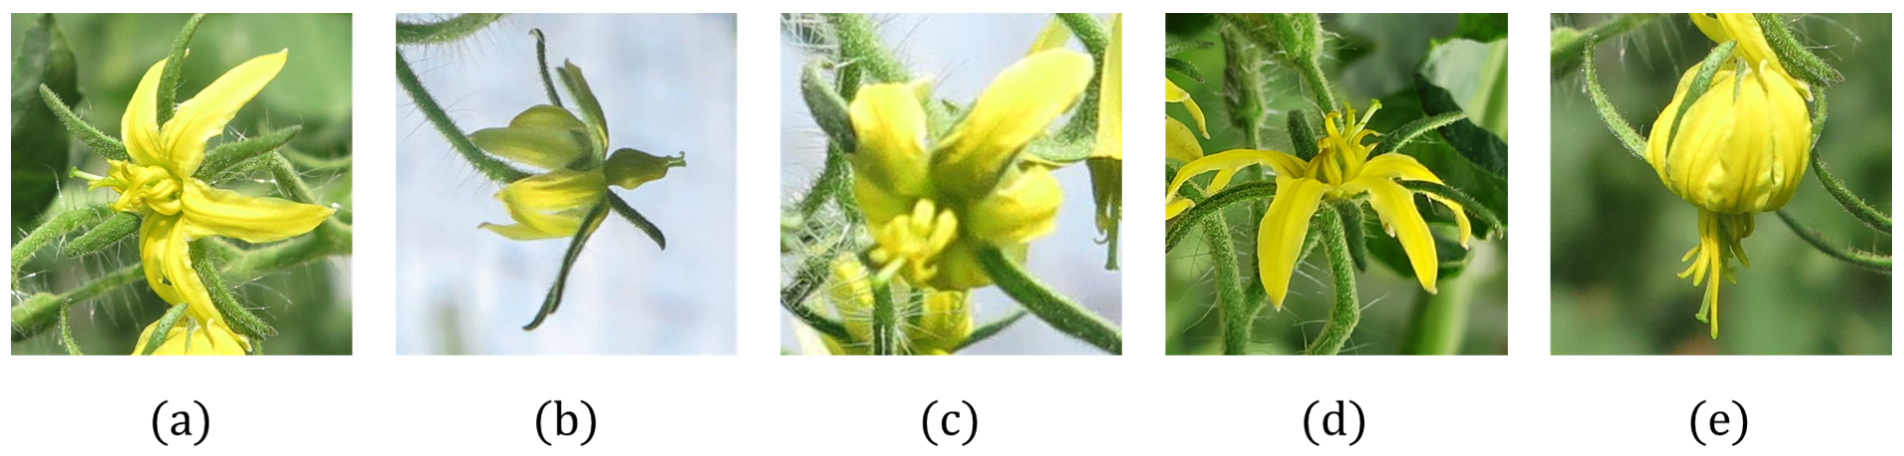
\includegraphics[width=0.8 \textwidth]{direct_f}
	\caption[不同朝向番茄和实例]{不同朝向番茄和实例,(a)朝左,(b)朝右,(c)朝前,(d)朝上,(e)朝下} % 中括号中内容为插图索引中显示内容,可在题注内容过长时使用
	\label{fig:direction_f}
\end{figure}
在番茄花授粉任务中,准确估计花朵的朝向至关重要,因为机械臂的末端需要与番茄花保持在适当的角度范围内,以确保授粉的顺利进行。然而,由于植物生长的随机性以及光周期的影响,番茄花的外观可能存在较大差异,使得基于单一三维模型进行姿态估计变得困难。为了解决这一问题,本研究采用了环形平滑标签\cite{yang2023delivery}(CSL)方法,将旋转角度预测从数值回归问题转换为分类问题。具体而言,设定上、下、左、右、中五个朝向向量,如\cref{fig:direction_f}所示,并基于最邻近向量对花朵姿态进行分类预测,从而避免了边界问题导致的异常损失,同时保证不同角度的权值对等。

此外,该方法与YOLACT目标检测网络相结合,在进行目标分割检测的同时获取花朵的朝向标签,避免了额外引入独立姿态检测模块所带来的计算开销。这种方式不仅提高了计算效率,还优化了系统资源的利用。在授粉任务中,由于机械臂末端与花朵的朝向并不需要完全一致,而是只需保持在合理的角度范围内,因此采用离散化分类方法足以满足任务需求,同时降低了计算复杂度。

该方法的优势在于避免了数值回归方法可能导致的误差累积问题,同时减少了计算资源消耗,提高了推理速度。此外,它适用于不同生长状态的番茄花,使得授粉任务能够在复杂场景下保持稳定。综合来看,该方法有效地解决了花朵姿态估计问题,并能够满足手眼协调机械臂在精准授粉任务中的应用需求。

\section{实验设计与结果分析}

\subsection{实验环境}
本章实验的软硬件设备如表下所示:

\begin{table}[htbp]
	\centering
	\caption[对称空间位姿重建实验环境]{对称空间位姿重建实验环境}
	\begin{tabularx}{\textwidth}{YYY}
		\toprule
		\textbf{序号} & \textbf{设备} & \textbf{型号} \\
		\midrule
		1 & RGB-D 深度相机 & RealSense D435i \\
		2 & 机械臂 & UR5 \\
		3 & 计算平台 & Ubuntu 20.04 + Python 3.8 \\
		4 & 深度学习框架 & PyTorch \\
		5 & 目标检测模型 & YOLACT \\
		6 & 手眼标定工具 & OpenCV \\
		\bottomrule
	\end{tabularx}
	\label{tab:spacerebuild}
\end{table}


\subsection{数据采集}
\subsubsection{数据采集环境搭建}
 \begin{figure}[htb]
	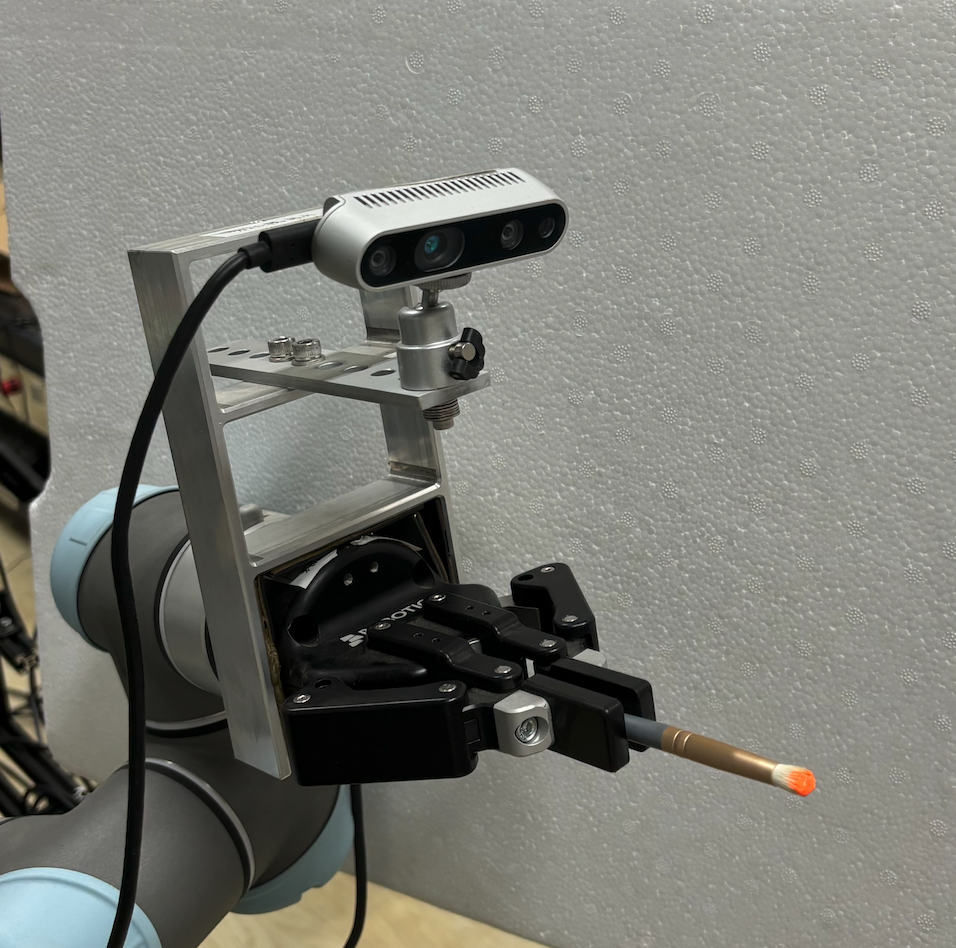
\includegraphics[width=0.4 \textwidth]{eye-in-hand}
	\caption[眼在手上实验环境搭建]{眼在手上实验环境搭建} % 中括号中内容为插图索引中显示内容,可在题注内容过长时使用
	\label{eye-in-hand}
\end{figure}
机械臂的末端安装深度相机,采用 Eye-in-Hand(眼在手上) 方式,使相机随机械臂运动,以便在不同角度和位置采集目标物体的RGB-D数据,如\cref{eye-in-hand}所示。此外,实验环境模拟农业应用场景,选择多株番茄植株,并在实验区域布置不同姿态的番茄花,以测试方法在真实应用中的适用性。

为了确保实验的可重复性,实验在两种光照条件下进行:(1)稳定光照环境,即在固定的室内实验室中,以恒定照明条件采集数据;(2)变化光照环境,即在模拟户外或半开放环境下,通过改变光源角度和强度,测试算法在不同光照条件下的鲁棒性。此外,为了验证该方法在不同背景复杂度下的适应性,实验设置了单一背景(纯色背景)和复杂背景(包含叶片、枝条等干扰因素)的场景。

\subsubsection{手眼标定数据采集}
 \begin{figure}[htb]
	\includegraphics[width=0.8 \textwidth]{eye-in-hand.drawio.png}
	\caption[采集标定数据示例图]{采集标定数据示例图} % 中括号中内容为插图索引中显示内容,可在题注内容过长时使用
	\label{eye-in-hand1}
\end{figure}

在实验中,手眼标定用于确定相机坐标系与机械臂末端坐标系之间的变换关系,以确保机械臂能够基于视觉感知信息进行精确操作。本实验采用 Eye-in-Hand(眼在手上) 配置,即在机械臂(UR5)的末端安装 Intel RealSense D435i 深度相机,使相机与机械臂同步运动,从不同角度观察目标物体。为保证标定的精度,实验通过多次数据采集,计算出相机相对于机械臂末端的位姿变换矩阵。

数据采集的核心步骤包括机械臂运动控制、图像采集、位姿记录和数据存储。首先,机械臂按照预设轨迹移动至不同位置,每个位置的相机视角不同,以确保标定数据的多样性。在每个位姿点,深度相机拍摄目标点位图像,并使用 OpenCV 进行角点检测,从而获取目标点位在相机坐标系下的三维坐标信息。同时,机械臂的关节编码器记录当前末端在基座坐标系下的位置与姿态,形成完整的数据对,如\cref{eye-in-hand1}所示。所有采集的数据存储为结构化格式,包括机械臂末端的位姿矩阵和相机观测到的目标点位坐标向量,以便后续计算。

在数据采集过程中,为了保证标定精度,实验采取了一系列质量控制措施。首先,确保目标点位在不同视角下均能被完整检测,避免数据偏差。其次,控制机械臂的运动稳定性,避免因震动或误差积累影响标定结果。对于图像采集环节,实验检查角点检测的稳定性,若发现某些视角的检测误差较大,则重新采集数据,以确保输入数据的准确性。

\subsubsection{深度图像数据采集}
本章实验中深度图像数据来自\ref{sec:dataset}中的数据集,故在此不重复叙述。

\subsection{实验设计}
本实验旨在提高机器人视觉系统的感知能力,通过深度图像噪声处理、手眼标定及目标朝向估计优化位姿计算精度,为机器人精准操作提供可靠的数据支持。实验主要涵盖三个部分,分别针对深度数据质量优化、相机与机械臂坐标转换精度评估以及目标朝向预测准确性进行验证。

在深度图像噪声处理实验中,首先采集多个场景的深度图像,包括光滑表面、复杂纹理表面以及具有透明、反射特性的物体,以分析不同目标的深度噪声特性。实验在稳定光照和变化光照环境下进行,评估深度图像的误差分布、空洞区域及边界失真情况。为了提升深度数据质量,实验采用 密度峰值去噪方法,对比 双边滤波 和 中值滤波 的去噪效果,统计去噪前后点云的完整性、曲面平滑度以及误差降低幅度。预期结果是密度峰值去噪能显著减少噪声点,提高点云的连续性,从而优化机器人基于深度信息的三维重建效果。

在手眼标定实验中,实验采用 Eye-in-Hand(眼在手上) 配置,即在机械臂末端安装深度相机,随机械臂运动观察标定板,以求解相机坐标系到机械臂末端坐标系的变换矩阵。实验选取 10-20 个不同位姿 采集数据,记录机械臂末端的运动轨迹,并通过 OpenCV 计算目标点位在相机坐标系下的位姿信息。随后,实验采用最小二乘优化算法 计算变换矩阵,并评估其误差,主要包括平移误差和旋转误差。

在目标朝向估计实验中,实验采集不同朝向的番茄花 RGB-D 图像,并手动标注其真实朝向(上、下、左、右、前)。采用 YOLACT 目标检测网络 进行目标分割,并结合 环形平滑标签(CSL)方法 预测朝向,以减少传统数值回归方法的边界误差问题。实验设计对比 CSL 方法和数值回归方法的分类准确率,并分析误分类情况,统计误分类角度的分布范围。


\subsection{实验结果与分析}
\subsubsection{深度图像去噪}
\begin{table}[htbp]
	\centering
	\caption[连续像素区域去噪前后数值对比]{连续像素区域去噪前后数值对比}
	\begin{tabularx}{\textwidth}{YYY}
		\toprule
		\textbf{序号} & \textbf{去噪前(深度 mm)} & \textbf{去噪后(深度 mm)} \\
		\midrule
		1  & 354.21 & 354.21 \\
		2  & 354.20 & 354.20 \\
		3  & 354.19 & 354.19 \\
		4  & 354.20 & 354.20 \\
		5  & 354.20 & 354.20 \\
		7  & \textcolor{red}{675.89} & 354.20 \\
		8  & \textcolor{red}{675.90} & 354.20 \\
		9  & 354.18 & 354.18 \\
		10 & 354.19 & 354.19 \\
		11 & 354.21 & 354.21 \\
		\bottomrule
	\end{tabularx}
	\label{tab:noise1}
\end{table}

深度图像去噪的主要目的是去除噪声异常点,减少因环境影响导致的深度数据突变,使深度图像更加平滑。\cref{tab:noise1}表示使用密度峰值去噪后,一组连续像素点去燥前后的数值变化。

实验结果表明,在去噪前,该区域的大部分深度值稳定在 354.20 mm 左右,但在第 7 和 8 行 出现了异常深度值 675.89 mm 和 675.90 mm,远超周围像素点的数值范围。这些异常点可能是由于空洞、环境光照干扰或物体材质特性导致的。经过密度峰值去噪处理后,这些异常点被成功修正回 354.20 mm,与周围像素值保持一致,而原本正常的深度数据未受影响。这一结果说明,密度峰值去噪方法能够精准检测并修正异常值,同时保持正常数据的完整性,避免对整体深度图像造成额外干扰。
\begin{table}[htbp]
	\centering
	\caption[局部区域去噪前后均方误差和方差]{局部区域去噪前后均方误差和方差}
	\begin{tabularx}{\textwidth}{YYY}
		\toprule
		\textbf{去噪阶段} & \textbf{均方误差(MSE)} & \textbf{方差(Variance)} \\
		\midrule
		去噪前 & 2.21 & 1.18 \\
		去噪后 & 1.66 & 0.79 \\
		\bottomrule
	\end{tabularx}
	\label{tab:noise2}
\end{table}


为了进一步量化去噪方法的效果,实验计算了去噪前后的均方误差和 方差,如\cref{tab:noise2}所示,分别用于衡量去噪后数据与真实值的偏差,以及去噪前后深度数据的波动程度。实验结果表明,去噪前局部区域的均方误差为 2.21 mm²,去噪后降低至 1.66 mm²,误差减少 24.9\%。这表明去噪方法能够有效减少深度数据的测量误差,使其更接近真实值。此外,去噪前的方差为 1.18,去噪后降至 0.79,减少 33.1\%,表明去噪后的深度数据更加稳定,局部区域的深度波动性明显降低。

\subsubsection{空间映射}
\begin{table}[htbp]
	\centering
	\caption[用于计算手眼变换矩阵的观测数据]{用于计算手眼变换矩阵的观测数据}
	\begin{tabularx}{\textwidth}{
			>{\hsize=0.3\hsize\centering\arraybackslash}Y
			>{\hsize=1.8\hsize\arraybackslash}Y
			>{\hsize=1.1\hsize\arraybackslash}Y
			>{\hsize=0.8\hsize\arraybackslash}Y}
		\toprule
		\textbf{序号} & \textbf{TCP 坐标} & \textbf{相机坐标} & \textbf{基座标} \\
		\midrule
		1 & [14, -280, 245, 0.066, -1.445, 2.814] & [-0.002, -0.046, 0.343] & [49, -427, 434] \\
		2 & [14, -280, 245, 0.066, -1.445, 2.814] & [0.076, -0.105, 0.351]  & [-25, -419, 496] \\
		3 & [14, -280, 245, 0.066, -1.445, 2.814] & [0.097, -0.003, 0.398]  & [-50, -490, 411] \\
		4 & [14, -280, 245, 0.066, -1.445, 2.814] & [-0.001, 0.000, 0.533]  & [48, -613, 438] \\
		\bottomrule
	\end{tabularx}
	\label{tab:eye-in-hand2}
\end{table}


为了提高标定精度,本实验首先对采集数据进行筛选,剔除误差较大的数据点。采用3σ 原则对数据误差进行筛选,即剔除误差超过均值 ±3 倍标准差的点,并利用欧氏距离检测剔除突变点, \cref{tab:eye-in-hand2}为剔除突变后的一组数据。数据筛选完成后,使用\cref{equ:hand-in-eye2}计算相机坐标系到机械臂末端坐标系的变换矩阵$X$,随后采用重投影误差评估标定精度,验证优化后的标定矩阵转换的精度,由\cref{equ:hand-in-eye3}计算重投影后目标点的坐标。
\begin{equation}
	\label{equ:hand-in-eye3}
	T = T_{tcp}^{base} \cdot T_{target}^{camera} \cdot X
\end{equation}

其中 $T_{tcp}^{base}$为tcp坐标,$T_{target}^{camera}$为目标点位的相机坐标,$X$为计算的到手眼转换矩阵。
\begin{table}[htbp]
	\centering
	\caption[重投影坐标与真实坐标对比]{重投影坐标与真实坐标对比}
	\begin{tabularx}{\textwidth}{YYY}
		\toprule
		\textbf{观测点位} & \textbf{重投影坐标(m)} & \textbf{真实坐标(m)} \\
		\midrule
		1 & [0.0404, -0.0453, 0.4220] & [0.0402, -0.0450, 0.4219] \\
		2 & [0.0972, -0.0038, 0.3980] & [0.0971, -0.0037, 0.3983] \\
		3 & [0.0752, -0.0573, 0.5390] & [0.0753, -0.0572, 0.5390] \\
		4 & [-0.2000, 0.0226, 0.3872] & [-0.2002, 0.0224, 0.3873] \\
		\bottomrule
	\end{tabularx}
	\label{tab:eye-in-hand3}
\end{table}
 \cref{tab:eye-in-hand3}为一组重投影坐标与真实坐标对比。实验结果表明,重投影坐标与真实坐标的误差极小,例如,第一个观测点的重投影坐标为 $[0.0404, -0.0453, 0.4220]$,而真实坐标为 $[0.0402, -0.0450, 0.4219]$,误差控制在 0.3 mm 以内。所有观测点的最大误差均不超过 0.5 mm,表明标定矩阵计算精确,适用于高精度任务。实验结果进一步证明,优化后的标定矩阵能够有效减少误差,使机械臂在不同视角下能够精准感知目标物体的位置。
 
 \section{本章小节}
 本章提出了一种基于对称虚拟空间的位姿重建方法,旨在解决农业场景中机械臂授粉任务对三维感知精度与实时性的双重需求。通过引入密度峰值去噪方法,显著提升了深度图像的稳定性与重建精度,有效剔除异常点并增强点云一致性。在手眼标定过程中,构建了Eye-in-Hand系统架构,采用多位姿数据采集与误差优化策略,实现了高精度的坐标系变换矩阵求解。针对番茄花多样朝向的挑战,采用环形平滑标签方法,将姿态估计转化为分类问题,结合YOLACT目标检测模型高效预测目标朝向。
 
 实验在不同光照和背景条件下验证了所提方法的鲁棒性与实用性,深度去噪使得局部区域均方误差减少24.9\%,方差降低33.1\%;手眼标定误差控制在0.5mm以内;目标朝向分类方法展现出更高的稳定性和抗干扰能力。整体系统能够为后续的授粉路径规划与柔顺控制提供高质量的三维位姿数据支撑。
    % !Mode:: "TeX:UTF-8"

\chapter{机械臂授粉运动的柔顺控制}\label{ch:5}
\section{引言}
在精准农业的发展背景下,机械臂在自动化授粉等复杂重复性作业中展现出显著的应用潜力。然而,授粉过程要求机械臂末端执行器与花朵结构进行精细接触,而花朵本身通常结构脆弱、空间分布不规则,并对外力高度敏感。这些特点对机械臂的运动规划与控制策略提出了更高要求,尤其是在非结构化农业环境中,挑战尤为突出。

为应对上述挑战,柔顺控制逐渐成为机械臂授粉任务中的关键研究方向。与传统刚性轨迹控制方法不同,柔顺控制强调机械臂对环境的动态适应能力,即能够根据外部环境变化实时调整自身运动与交互力。在授粉任务中,柔顺控制具体表现为两个核心要求:(1)机械臂需沿平滑、连续的轨迹逐步接近花朵,避免突变加速或震动;(2)在接触过程中,应施加轻柔、可调节的接触力,确保花粉能够有效传递至花柱,同时避免损伤花体结构。

实现柔顺控制需要多项关键技术的协同融合。首先,机械臂的运动路径不仅要优化作业效率,还需具备良好的连续性和平滑性,常采用样条插值或高阶多项式轨迹生成方法进行路径细化。其次,引入可编程的力控制机制,使系统能够根据不同花朵的品种、结构和姿态,实时调节末端施力大小。第三,通过视觉伺服系统实现对末端执行器姿态的实时修正,特别是在接近花朵末端的精细操作阶段。最后,系统需具备任务状态跟踪能力,对已授粉与未授粉花朵进行有效管理,实现闭环控制与顺序执行。

本章将系统性地提出一套面向机械臂授粉任务的柔顺运动控制策略。该策略融合路径规划优化、自适应力控、视觉伺服调整以及轨迹插值方法,旨在实现机械臂授粉过程的安全性、柔顺性与高效率。通过对算法实现与实验结果的分析,验证所提出方法在实际农业环境中的可行性与鲁棒性。

\section{方法}
\subsection{工作流程系统设计}
\begin{figure}[htb]
	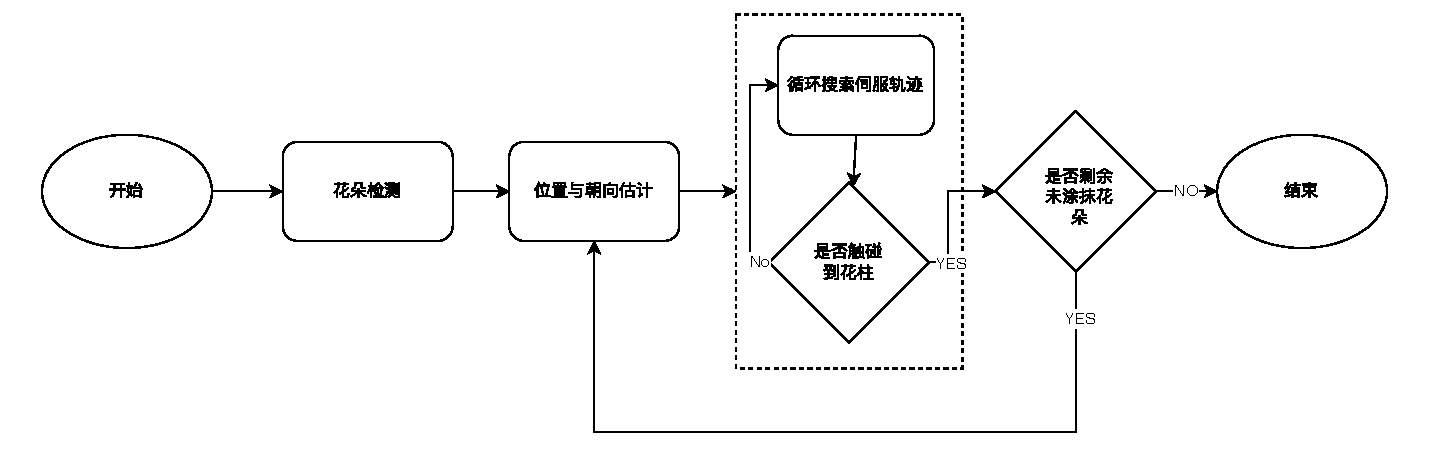
\includegraphics[width=1 \textwidth]{flowchat}
	\caption[柔顺授粉系统工作流程]{柔顺授粉系统工作流程} % 中括号中内容为插图索引中显示内容,可在题注内容过长时使用
	\label{fig:flowchat}
\end{figure}
本研究设计了一个本端到端的视觉引导柔顺授粉控制架构系统,其整体流程如\cref{fig:flowchat}所示。系统首先启动视觉感知模块,通过RGB-D相机对植物花朵进行实时采集,并基于\ref{dectection}和\ref{sec:rebuild}中的方法估计图像中所有花朵的空间位置及其朝向,将图像坐标转换为世界坐标,完成对待授粉花朵的三维定位与姿态估计。

获取到全部待授粉花朵的位置与姿态后,系统进入路径规划与分步控制阶段。首先通过插值路径控制策略,指引机械臂末端刷头从当前位置运动至目标花朵附近,完成粗略接近。此后,系统启动基于圆形搜索轨迹的精细伺服控制模块,根据待授粉花朵花柱中心点在图像平面中构造多个伺服点,逐个推进花粉刷完成柔顺接触。

在伺服过程中,系统实时采集末端视角图像,并调用Inception-v3图像分类网络判断是否完成雌蕊接触。若判定为“已触碰”,则标记当前花朵为“已授粉”,并判断是否仍有其他待处理花朵;若仍有剩余目标,则系统重新进入定位与控制循环;否则,流程终止。该流程实现了从花朵识别、空间感知、路径规划到触觉判断的全过程自动化控制,具备良好的柔顺性与任务闭环能力。


\subsection{两阶段伺服控制}
在实现精准授粉操作时,单纯依赖一次性定位完成花粉刷与雌蕊的接触存在较大不确定性,尤其是在自然环境下花朵存在微小摆动、定位误差以及执行器精度限制的情况下。为此,本研究提出一种粗到精的两阶段伺服控制策略,分别对应于“花朵接近”与“精细伺服”两个阶段,旨在提升授粉操作的柔顺性与鲁棒性。

在第一阶段中,系统根据视觉检测模块提供的雌蕊三维位置与姿态信息,计算出机械臂末端的目标位姿,并通过逆运动学求解机械臂的关节角度,使机械臂从当前位置平稳地移动到距离待授粉花柱一定安全距离处。在该阶段,花粉刷并不与待授粉花朵发生直接接触,而是通过一次全局路径规划将其引导至花朵附近,完成粗定位。

在完成初步定位后,系统进入第二阶段,即精细伺服控制阶段。在该阶段中,花朵与末端刷头已共同出现在相机视野中,系统利用检测到的雌蕊朝向信息对花粉刷进行旋转,使其姿态尽可能与雌蕊法向垂直,从而确保后续接触方向与授粉生理要求一致。随后,系统启动一种圆形搜索轨迹伺服策略,以覆盖可能存在的定位误差和花朵抖动带来的偏差。


\begin{figure}[htb]
	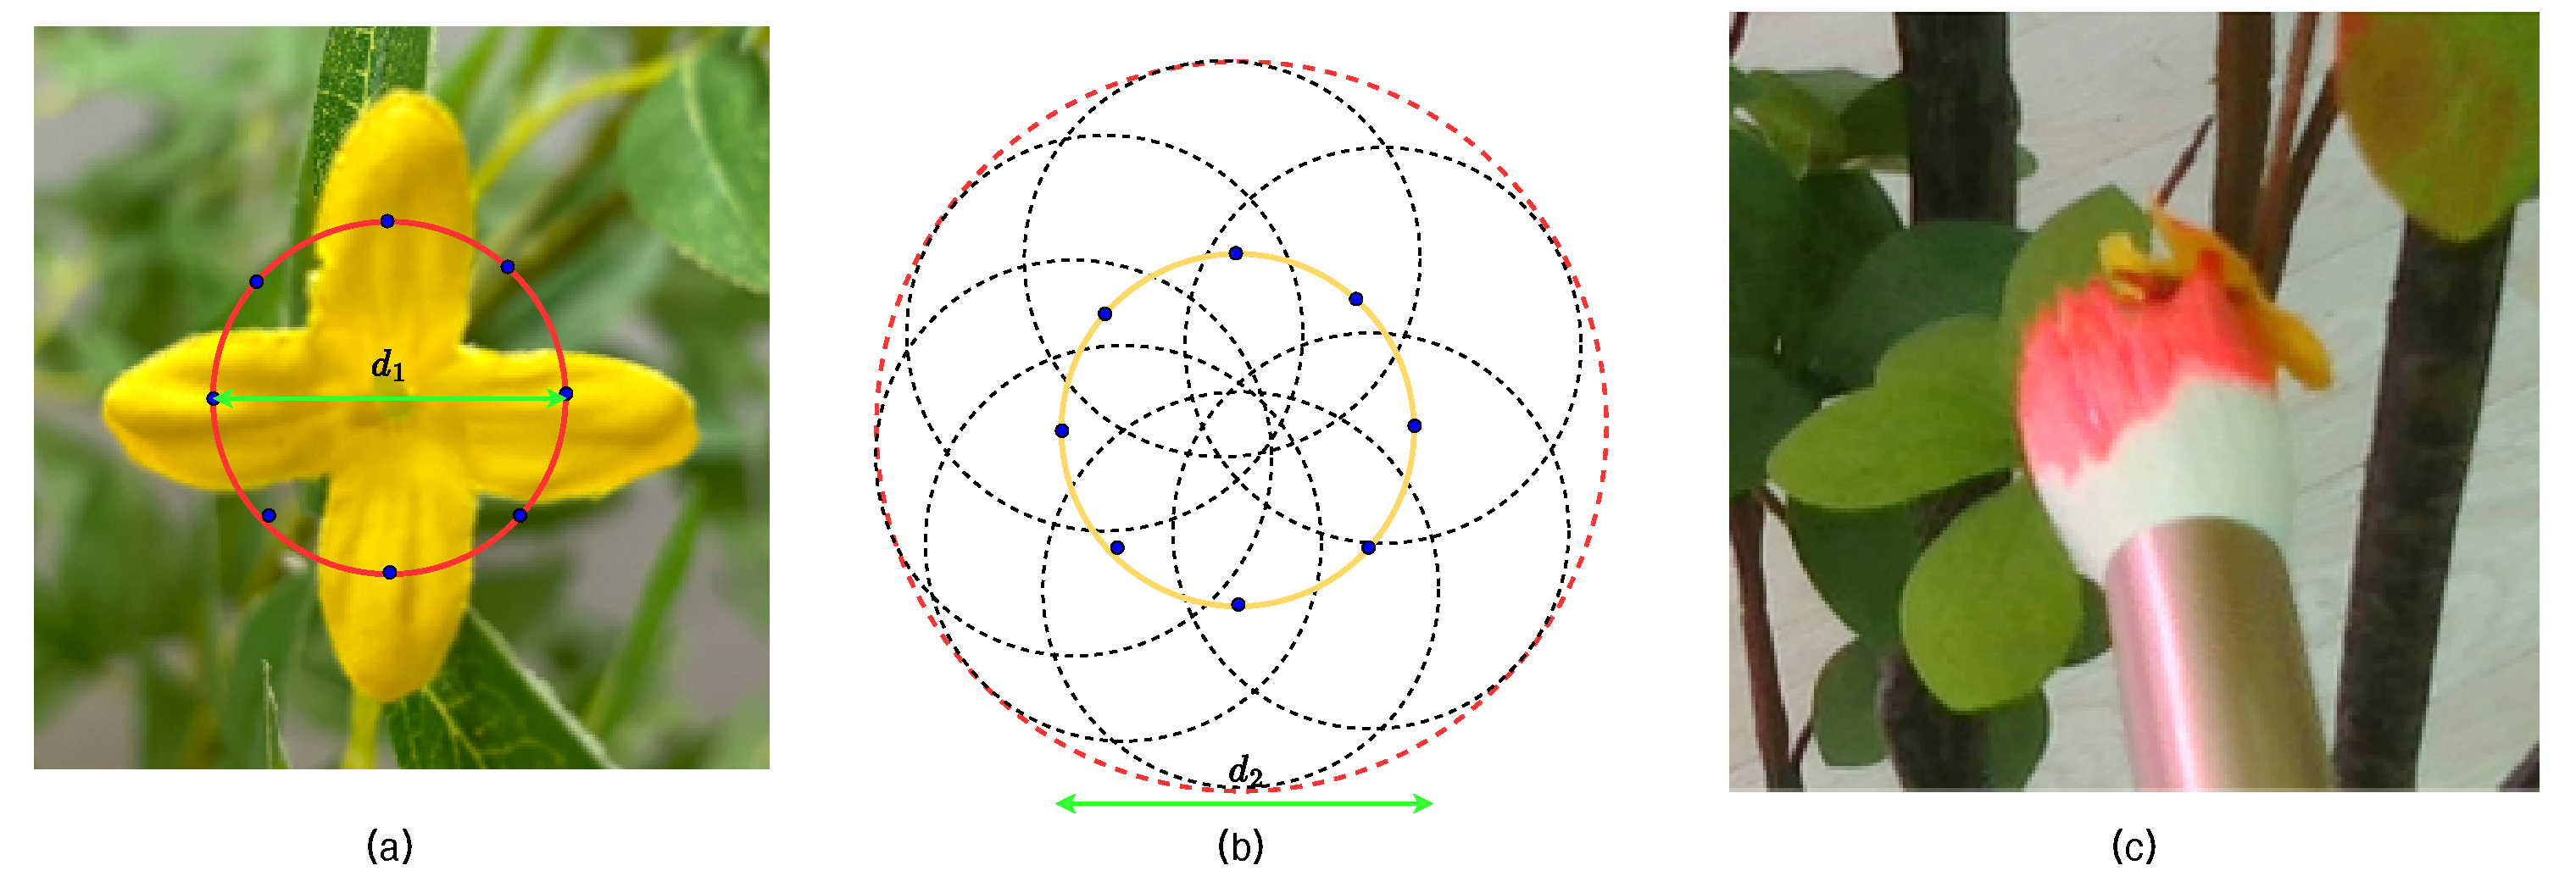
\includegraphics[width=1 \textwidth]{servoing}
	\caption[圆形搜索轨迹示意图]{圆形搜索轨迹示意图} % 中括号中内容为插图索引中显示内容,可在题注内容过长时使用
	\label{fig:servoing}
\end{figure}

圆形搜索轨迹伺服策略策略借鉴了Hanwen Kang提出的螺旋式伺服策略的思想,在待授粉花朵图像中心点的平面上构造一个大圆,并在其边缘等距布置八个伺服点,逐个依次控制花粉刷前进至这些点。\cref{fig:servoing}中(a)图中的红色大圆表示搜索路径,(b)图中黑色虚线表示搜索覆盖范围,此策略不仅在图像平面中进行二维伺服,还在三维空间中沿着垂直于花面方向长度为$K$,等间距布置多个圆轨迹层,构成一个圆柱形的伺服搜索体积,从而实现对雌蕊区域的空间覆盖。整个伺服空间体积可表示为:
\begin{equation}
	\label{equ:servoing_volum}
    V = \pi \cdot K \cdot d \cdot \frac{(d_{1}+d_{2})^{2}}{4}
\end{equation}

在伺服过程中,为了判断花粉刷是否已经成功接触到待授粉花朵,系统引入了图像识别模块,对当前相机视图进行分类。具体实现采用轻量级神经网络结构Inception-v3,对每一帧图像进行二分类,判断是否出现“已触碰”状态。一旦图像分类模型识别出刷头成功接触雌蕊,系统立即终止当前伺服动作,并将该花朵标记为“已授粉”,随后进入下一个待处理的目标花朵,\cref{fig:servoing}中(c)图表示已触碰状态。
这种粗到精的分级控制方式将全局路径优化与局部伺服精调有机结合,在保证作业效率的同时,显著提升了授粉的精确性与柔顺性,尤其适用于自然环境中具有高动态变化和复杂几何结构的植物授粉任务。

\subsection{基于三次样条插值的关节空间柔顺运动控制}
在机械臂执行授粉任务过程中,为了避免在目标切换时出现剧烈加速、减速带来的震动与力冲击,我们在“花朵接近”阶段引入了三次样条插值方法,用于生成平滑、连续的运动轨迹,确保系统整体的柔顺性和安全性。系统首先根据花朵空间位置估计模块提供的多个花朵位姿,利用TSP算法生成最优访问路径,然后将每对相邻花朵作为一段插值区间。在每一段区间中,系统以起点和终点的关节角度作为约束,根据\cref{equ:Cubic Spline Interpolation 2}构造三次样条插值函数。

插值轨迹的求解过程采用自然边界条件(即起止段加速度为0),通过构造并求解一个线性方程组,计算出每段插值曲线的系数。生成的轨迹再经过离散化处理,逐步下发到机械臂控制执行,最终驱动机械臂平稳地从当前花朵移动到下一朵花的附近位置,完成粗略接近。

这种插值策略在不依赖复杂优化算法的前提下,实现了对机械臂运动轨迹的高质量柔顺控制,特别适合在开放空间内进行的连续多目标作业场景。与伺服控制阶段形成互补,一方面负责大范围、低精度、连续性的轨迹生成,另一方面实现小范围、高精度、响应性的接触动作,共同构成完整的授粉控制闭环。

\section{实验设计与结果分析}
为了验证本章提出的基于插值轨迹与精细伺服策略的柔顺授粉控制方法的有效性,本文搭建了一个实际授粉实验平台,并在温室环境中对12株植物进行了多轮真实授粉测试。实验围绕机械臂在实际环境中对多朵花朵进行柔顺接近、伺服接触与结果评估展开,重点考察系统的任务完成率、操作精度、时间成本与算法表现。
\subsection{柔顺授粉实验环境搭建}
\begin{figure}[htb]
	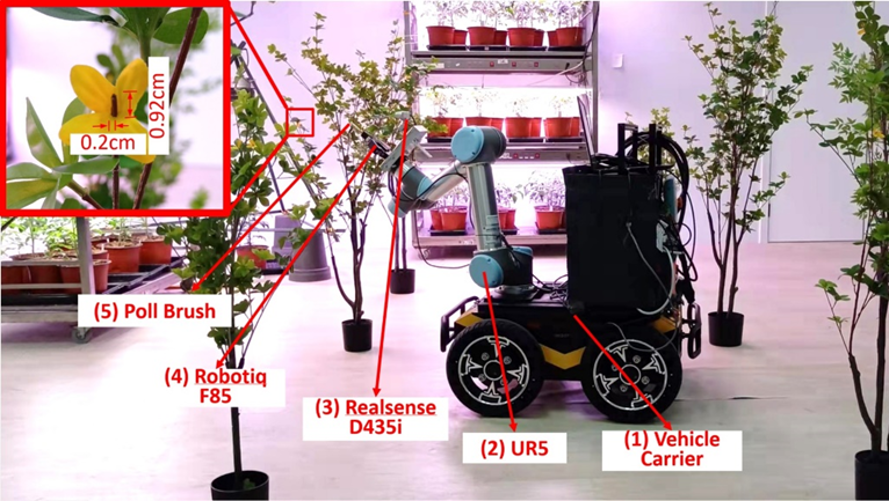
\includegraphics[width=1 \textwidth]{robot_env.jpg}
	\caption[柔顺授粉实验环境搭建]{柔顺授粉实验环境搭建} % 中括号中内容为插图索引中显示内容,可在题注内容过长时使用
	\label{fig:robot_env}
\end{figure}
为了验证本章提出的机械臂柔顺授粉控制方法的有效性,我们在室内环境下搭建了一个集感知、控制与执行于一体的授粉实验平台。该平台由移动底盘、机械臂、授粉末端、视觉感知系统以及控制计算单元等多个模块组成,具备在实际场景中完成自动化授粉任务的能力。

如\cref{fig:robot_env}所示,整个平台以MR1000 轮式移动机器人为基础构建。在平台上安装了一台 Universal Robots UR5 六自由度协作机械臂,其工作半径为 850 mm,最大负载为 5 kg,具备良好的空间覆盖性和运动灵活性,能够应对植物多样的开花方位与空间结构。UR5 的末端安装了 Robotiq F85 自适应夹爪,用于夹持柔软的羊毛材质花粉刷。该花粉刷形状为长 3.0 cm、直径 2.0 cm 的圆柱体,其末端连接有一个直径为 2.0 cm 的球状羊毛刷头,具备良好的生物兼容性与柔软接触特性,可有效避免在触碰花柱时对花朵造成损伤。为了实现视觉感知与闭环伺服控制,我们在机械臂末端安装了一台 Intel RealSense D453i RGB-D 相机,用于采集彩色图像与深度信息。该相机既用于在检测植物花朵的位置与朝向,也用于伺服控制阶段判断刷头是否接触到花柱,实现完整的视觉引导与反馈闭环。

系统的计算与控制单元由一台搭载 NVIDIA RTX 4050 显卡的便携式电脑组成,集成了多个感知与控制模块。其中包括用于花朵检测的模型、用于花柱方向识别的网络,以及用于触碰判别的分类网络,支持端到端自动化作业流程。该控制系统通过与机械臂驱动器的通信接口,实时下发插值轨迹与伺服指令,实现对多朵花朵的连续、柔顺授粉控制。
本实验采用的软硬件于下表中列出:
\begin{table}[htbp]
	\caption[柔顺授粉控制软硬件]{柔顺授粉控制软硬件}
	\setlength{\tabcolsep}{14mm}{ % 因表格过窄,手动设置宽度为7mm
		\begin{tabular}{clc}
			\toprule
			序号    &  设备    & 型号   \\
			\midrule
			1 & 操作系统 & windows10 \\
			2 & cpu & intel13450X \\ 
			3 & 显卡 & NVIDIA GeForce RTX4050 \\
			4 & 运载底座  & MR1000    \\
			5 & 机械臂  & UR5    \\
			6 & 相机 & realsense  \\
			7 & 夹爪  & Robotiq F85    \\
			8 & 授粉刷     & /  \\
			9 & 授粉植株     & / \\
			\bottomrule
	\end{tabular}}
	\label{tab:pollination_env}
\end{table}
\subsection{实验设计}
为了系统验证所提出的基于插值与两阶段伺服控制的柔顺授粉方法的有效性,我们设计了对比实验,评估柔顺控制策略在实际应用中的表现提升程度。实验以是否采用柔顺控制策略作为主要对比变量,将系统分为两组:一组为对照组(未启用插值和伺服控制),另一组为实验组(采用本章提出的柔顺控制方法)。

实验场景设于室内环境,共布置12株植株,包含自然分布的121朵可授粉花朵。每组实验均在同环境中开展,确保目标花朵数量、空间分布、光照条件一致。每次试验过程中,机器人在完成对一株植物的检测、定位与路径规划后,依次对所有检测到的可授粉花执行授粉操作,并记录授粉成功率,授粉平均耗时指标。
其中,若刷头接触到花柱即记为“成功”,触碰花瓣但未触花柱记为“触碰未中”,完全未触及者记为“失败”。为客观评估授粉是否成功,我们使用蘸有红色颜料的花粉刷,通过残留痕迹判断是否成功接触花柱。
此外,我们分别记录系统中主要模块(花朵检测、花柱识别、位置转换、接近控制与伺服控制)的处理时间,并评估系统整体运行效率。
\subsection{结果与分析}
\begin{table}[htbp]
	\caption[授粉结果]{授粉结果}
	\setlength{\tabcolsep}{14mm}{ % 因表格过窄,手动设置宽度为7mm
		\begin{tabular}{ccc}
			\toprule
			评价指标    &  无柔顺控制    & 柔顺控制   \\
			\midrule
			授粉成功率(\%) & 82.3  & 96.5 \\
			总授粉次数(次) & 82 & 96 \\
			总尝试次数(次)& 158& 112 \\
			平均每花尝试次数(次) & 1.58& 1.12 \\
			单次授粉成功率(\%) & 51.9 & 85.7 \\ 
			单朵授粉耗时(s) & 30.1 & 18.9 \\
			\bottomrule
	\end{tabular}}
	\label{tab:pollination_env2}
\end{table}

\begin{figure}[htb]
	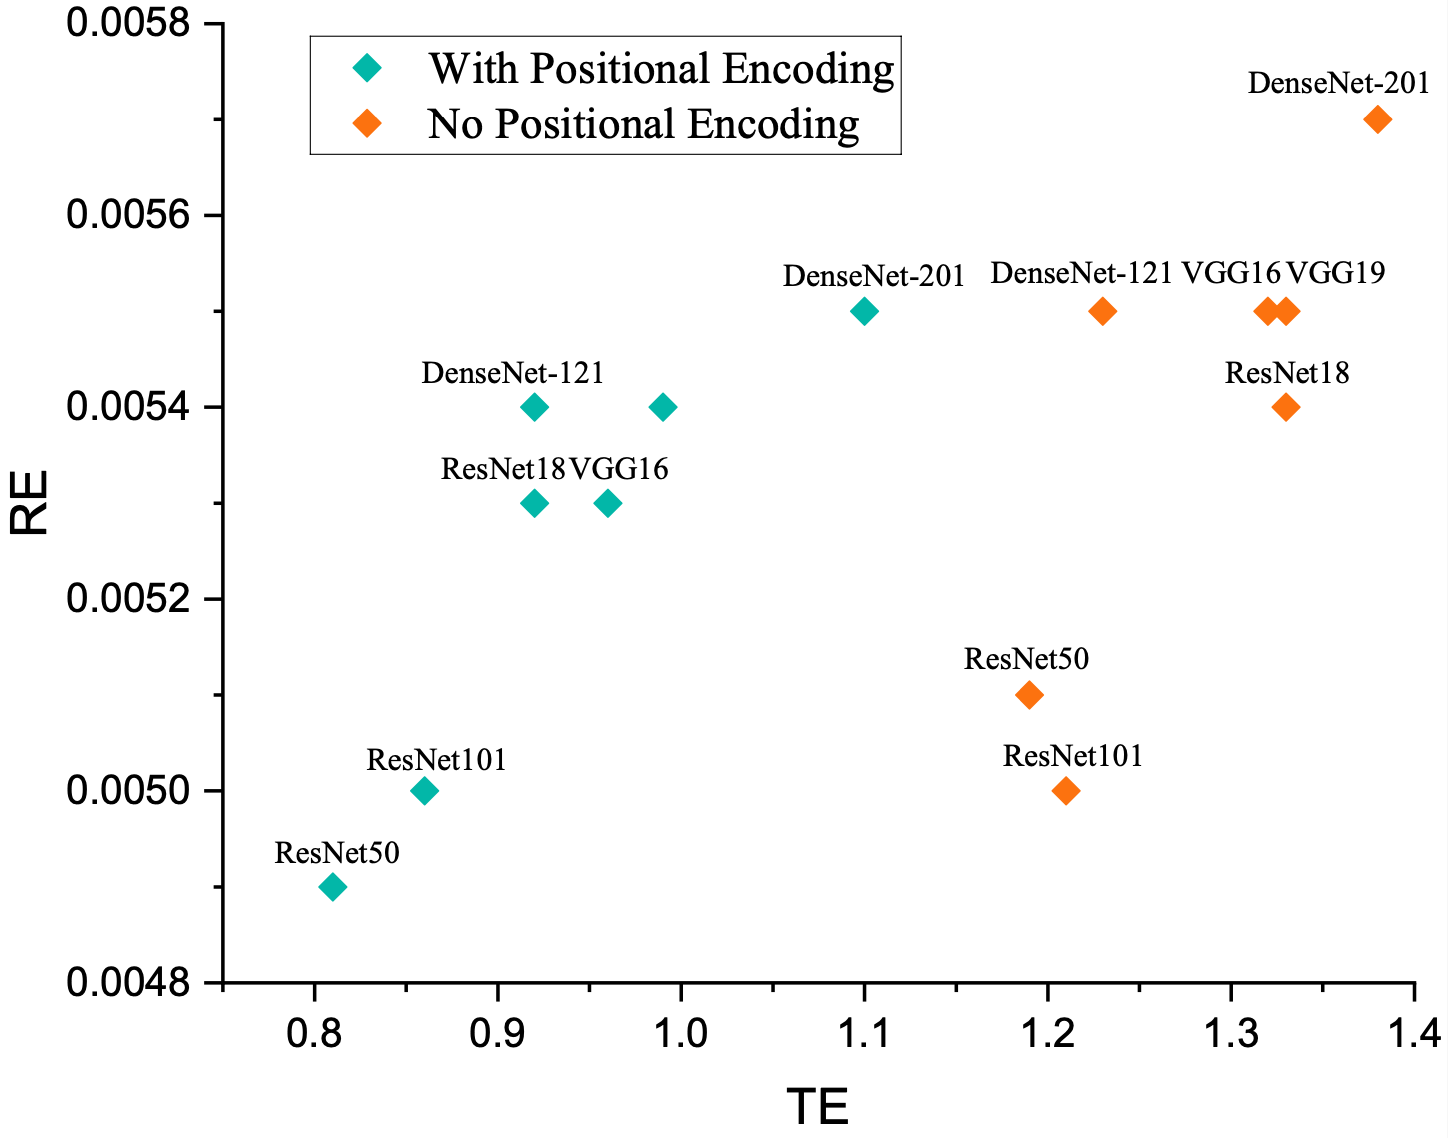
\includegraphics[width=1 \textwidth]{result}
	\caption[授粉实验结果主要指标对比]{柔顺控制实验结果主要指标对比} % 中括号中内容为插图索引中显示内容,可在题注内容过长时使用
	\label{fig:result4}
\end{figure}

从\cref{tab:pollination_env2}所列数据和\cref{fig:result4}显示结果可以看出,采用插值与两阶段伺服控制策略后,机械臂授粉系统在多个关键性能指标上均获得了显著提升。首先,在授粉效果方面,系统的授粉成功率由原始对照组的 82.3\% 提高至 96.5\%,说明插值路径与精细伺服策略有效提升了刷头与花柱之间的接触精度。同时,系统完成同样数量目标花朵的授粉所需的总尝试次数从 158 次下降至 112 次,平均每朵花的尝试次数由 1.58 次减少至 1.12 次,单次伺服成功率也从 51.9\% 提升至 85.7\%。这一变化表明,本方法在伺服过程中更为高效,命中率更高,减少了冗余伺服动作,有助于提升系统整体稳定性与节能性。

在系统执行效率方面,柔顺控制策略将单朵花的平均处理时间由 27.1 秒缩短至 18.9 秒,总任务耗时减少了约 30\%。这得益于插值方法在机械臂关节空间生成连续平滑的轨迹,使运动过程更加流畅,减少了运动过程中因关节越限而导致授粉无法继续的可能性。同时,视觉伺服阶段的快速定位与高命中率减少了重复调整的时间开销。

综合来看,插值与两阶段伺服控制策略的引入,在不增加系统结构复杂度的前提下,显著提升了机械臂在温室环境中的授粉能力。它不仅改善了机械臂的运动品质,也提升了系统的智能水平与任务闭环能力,为农业场景下的自动化操作提供了可靠支撑。该策略具备良好的通用性,适用于结构复杂、目标不确定性高的连续性操作任务。

    % !Mode:: "TeX:UTF-8"

\chapter{末端授粉效率的提高}\label{ch:6}
\section{引言}

在自主授粉机器人系统中,机械臂末端的定位精度直接影响授粉成功率与任务效率。由于农业场景中目标花朵小巧、分布密集、易受遮挡,且常缺乏深度信息,导致传统依赖点云建模或模板匹配的定位方法在末端对准精度上存在显著不足。

为了解决这一问题,本文提出一种基于 Transformer 的机器臂授粉末端平移和旋转误差预测方法,仅利用 RGB 图像输入,通过深度学习直接预测末端与目标花朵之间的三维平移与旋转误差。该方法可实时修正末端位姿,显著提升授粉效率并缩短伺服时间。

\section{方法}

\subsection{末端误差建模}
\begin{figure}[htb]
	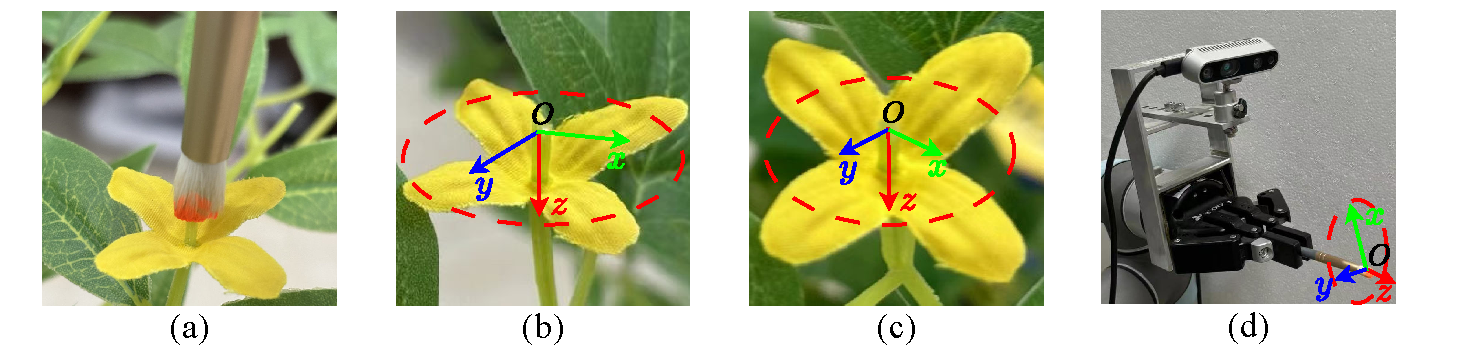
\includegraphics[width=1 \textwidth]{error}
	\caption[不同位置构建的笛卡尔坐标系]{不同位置构建的笛卡尔坐标系} % 中括号中内容为插图索引中显示内容,可在题注内容过长时使用
	\label{fig:effective1}
\end{figure}


为了描述平移偏差误差与姿态旋转偏差误差,需要分别在目标花朵与授粉机器人的末端构建两个笛卡尔坐标系,记为 $C_{A}$ 与 $C_{B}$。构建在花朵上的笛卡尔坐标系 $C_{A}$ 以柱头末端为原点 $O$,其 $x$ 轴与 $y$ 轴构成的平面与花瓣平面平行,$z$ 轴与柱头平行,指向花朵内部,如\cref{fig:effective1}中$b,c$ 所示。而构建在授粉机器人末端的笛卡尔坐标系 $C_{B}$,以刷头末端为原点 $O$,该坐标系通过对 UR5 机械臂的 TCP 坐标系进行平移获得,如图\cref{fig:effective1}中d 所示。$C_{A}$ 可以通过一个 $4\times4$ 的平移—旋转矩阵 $TR$ 从 $C_{B}$ 推导得到:
\begin{equation}
	\label{eq0_1}
	TR=
	\begin{bmatrix}
		R_{11} & R_{12} & R_{13} & t_{1} \\
		R_{21} & R_{22} & R_{23} & t_{2} \\
		R_{31} & R_{32} & R_{33} & t_{3} \\
		0 & 0 & 0 & 1 \\
	\end{bmatrix}
\end{equation}
\begin{equation}
	\label{eq0_2}
	C_{A} = TR\cdot C_{B}
\end{equation}

平移偏差误差与姿态旋转偏差误差分别为平移旋转矩阵 $TR$ 中的平移向量 $t$ 与由旋转矩阵 $R$ 推导出的旋转向量:
\begin{equation}
	\label{eq0_3}
	t = \begin{bmatrix}
		t_1  &	t_2 &	t_3
	\end{bmatrix}^\mathrm{T}
\end{equation}
\begin{equation}
	\label{eq0_4}
	R=
	\begin{bmatrix}
		R_{11} & R_{12} & R_{13}\\
		R_{21} & R_{22} & R_{23} \\
		R_{31} & R_{32} & R_{33} 
	\end{bmatrix}
\end{equation}


当授粉机器人末端处于理想授粉姿态时,平移偏差误差与旋转姿态偏差误差的数值趋近于零。此时,授粉机器人末端的刷头垂直于目标花朵的花瓣平面,恰好接触柱头,即坐标系 $C_{A}$ 与 $C_{B}$ 重合,如\cref{fig:effective1}中$a$ 所示。
\begin{equation}
	\label{eq0_4_1}
	\begin{split}
		\theta &= \cos^{-1}(\frac{trace(R) - 1}{2})\\
		\overrightarrow{V}&= \frac{1}{2\sin(\theta)}\begin{bmatrix}
			R_{32} - R_{23}\\
			R_{13} - R_{13} \\
			R_{21} - R_{12} 
		\end{bmatrix} \\
		\overrightarrow{W} &= \theta \overrightarrow{V}
	\end{split}
\end{equation}

模型预测的平移偏差误差与旋转姿态偏差误差分别记为 $\hat{t}$ 与 $\hat{R}$。末端执行器到目标花朵柱头之间的实际误差与预测误差之间的差值,分别作为平移误差($TE$)与旋转误差($RE$)进行计算。根据公式~(\ref{eq0_4_1}),旋转矩阵 $R$ 与 $\hat{R}$ 可被转换为旋转向量 $\overrightarrow{W}$ 与 $\hat{\overrightarrow{W}}$:
\begin{equation}
	\label{eq0_5}
	TE = \Vert \hat{t} -t \Vert \\
\end{equation}
\begin{equation}
	\label{eq0_6}
	RE = 1 -  \frac{\hat{\overrightarrow{W}}\overrightarrow{W}}{\Vert\hat{\overrightarrow{W}}\Vert\Vert\overrightarrow{W}\Vert}
\end{equation}

$TE$ 的单位为厘米(cm),表示预测平移误差与实际平移误差之间的空间距离;$RE$ 为无量纲量,表示预测旋转向量误差与实际旋转向量误差之间的余弦距离。

\subsection{基于Transformer的授粉末端误差估计网络}

为提高授粉机器人末端姿态估计的精度,本研究提出了一种基于Transformer的末端误差差估计网络。该网络以“手眼一体”RGB相机采集的图像作为输入,输出授粉末端相对于目标花朵在笛卡尔坐标系下的平移与旋转偏差向量 $(\Delta T_{x}, \Delta T_{y}, \Delta T_{z},\Delta W_{x}, \Delta W_{y}, \Delta W_{z})$,其中 $\Delta T$ 表示三维平移偏差,$\overrightarrow{W}$ 表示三维旋转向量偏差。


为了从图像中提取高质量的空间特征,模型采用了预训练的卷积神经网络作为特征提取模块。该网络能够有效捕捉图像中的空间层级信息,将原始图像转换为高维特征向量。随后,为保留图像的空间结构信息,模型在特征向量中引入了二维正弦位置编码,并将其与特征相加后输入至Transformer编码器中。

\begin{figure}[htb]
	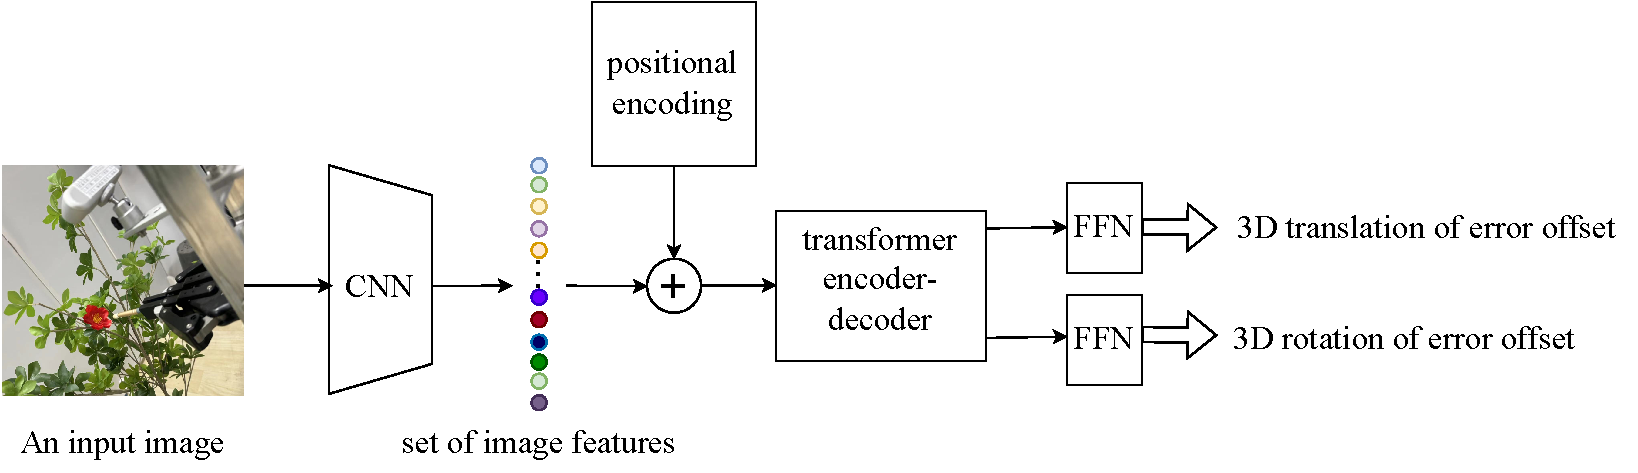
\includegraphics[width=1 \textwidth]{model}
	\caption[用于估计授粉末端平移和旋转误差的模型整体框架]{用于估计授粉末端平移和旋转误差的模型整体框架} % 中括号中内容为插图索引中显示内容,可在题注内容过长时使用
	\label{fig:effective3}
\end{figure}

\cref{fig:effective3} 展示了模型整体框架。首先,输入图像经过卷积神经网络(CNN)提取高维图像特征。随后,这些特征被加入位置编码后输入至 Transformer 模块中。Transformer 的输出特征分别由两个独立的前馈神经网络处理,用于分别预测平移偏差与旋转偏差。

在Transformer编码器中,采用了五头多头注意力机制以并行捕获不同子空间的信息。编码后的特征由解码器进一步处理,解码器通过查询机制将嵌入向量转换为用于预测的特征表示。最终,这些特征分别输入两个前馈神经网络中,分别用于回归平移偏差向量 $\Delta T$ 与旋转偏差向量 $\overrightarrow{W}$。

\begin{figure}[htb]
	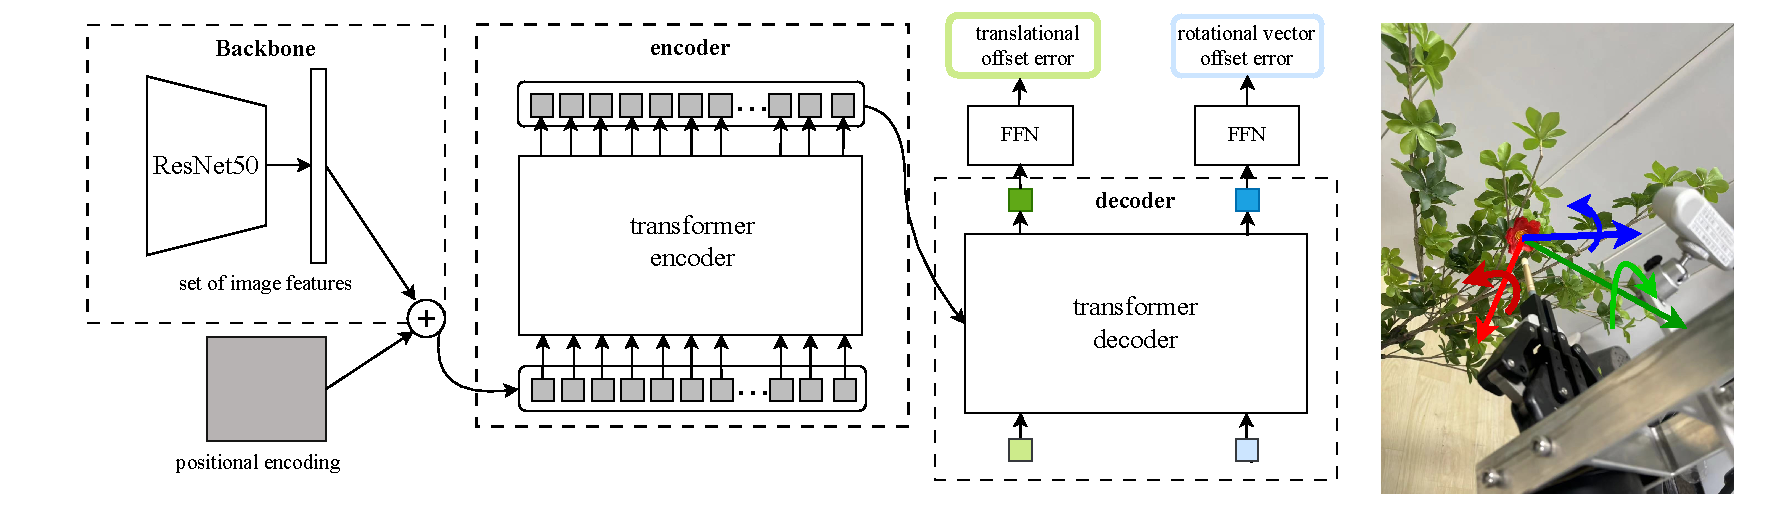
\includegraphics[width=1 \textwidth]{Architecture}
	\caption[用于估计授粉末端平移和旋转误差的模型结构]{用于估计授粉末端平移和旋转误差的模型结构
	} % 中括号中内容为插图索引中显示内容,可在题注内容过长时使用
	\label{fig:effective4}
\end{figure}
\cref{fig:effective4} 展示了完整网络结构,采用 ResNet50 作为主干网络,从输入图像中学习高层特征。这些特征随后与位置编码相结合,并输入至编码器中。随后,解码器首先输出一个用于预测平移偏差的特征向量,该向量作为输入传递给一个前馈神经网络进行平移偏差的回归预测。接着,该特征向量被用作查询输入,再次送入解码器,生成另一个特征向量,并由另一个独立的前馈神经网络用于旋转姿态偏差的预测。




\subsection{损失函数设计}
在本章所提出的模型中,分别对平移偏差误差与旋转姿态偏差误差进行预测,因此设计了两个独立的损失函数。第一个损失函数记为 $Loss_{T}$,用于度量模型所预测的授粉机器人末端相对于目标花朵柱头的空间位置偏差误差与实际空间偏差误差之间的均方差。$Loss_{T}$ 定义如下:
\begin{equation}
	\label{eq5}
	Loss_{T} = \frac{1}{2m}\sum\limits_{x\in\mathcal{M}}(\hat{T_{n}} - T_{n})^{2} 
\end{equation}

其中,$\mathcal{M}$ 表示测试数据集的集合,$m$ 为集合中的样本数,$\hat{T_{n}}$ 与 $T_{n}$ 分别表示模型预测的平移偏差误差与真实平移偏差误差。

第二个损失函数记为 $Loss_{R}$,用于衡量模型所预测的授粉机器人末端相对于目标柱头的空间旋转误差与实际旋转误差之间的差异。$Loss_{R}$ 定义如下:
\begin{equation}
	\label{eq6}
	Loss_{R} = \frac{1}{2m}\sum\limits_{x\in\mathcal{M}}(\frac{1}{\sigma_{1}^{2}}(\Vert\hat{\theta} -\theta \Vert^{2}) + \frac{1}{\sigma_{2}^{2}}(1 - \frac{\hat{\overrightarrow{V}}\overrightarrow{V}}{\Vert\hat{\overrightarrow{V}}\Vert\Vert\overrightarrow{V}\Vert}) + \log(\sigma_{1}\sigma_{2})) 
\end{equation}

其中,$\mathcal{M}$ 表示测试数据集的集合,$m$ 为集合中的样本数。变量 $\hat{\theta}$、$\theta$、$\hat{\overrightarrow{V}}$ 和 $\overrightarrow{V}$ 分别表示预测与真实旋转角度和旋转轴,$\sigma_{1}$ 与 $\sigma_{2}$ 为需要通过训练学习的可调参数。

最终用于模型训练的联合损失函数定义如下:
\begin{equation}
	\label{eq7}
	Loss =  \alpha Loss_{T} + \beta Loss_{R}
\end{equation}

该合损失函数综合衡量模型在训练过程中对平移偏差误差与旋转姿态偏差误差的拟合能力。其中,$\alpha$ 与 $\beta$ 为可调超参数,分别表示平移损失与旋转损失的加权系数,需在模型训练过程中进行系统性调整以获得最优性能。


\section{实验设计与分析}

\subsection{数据预处理}
\begin{figure}[htb]
	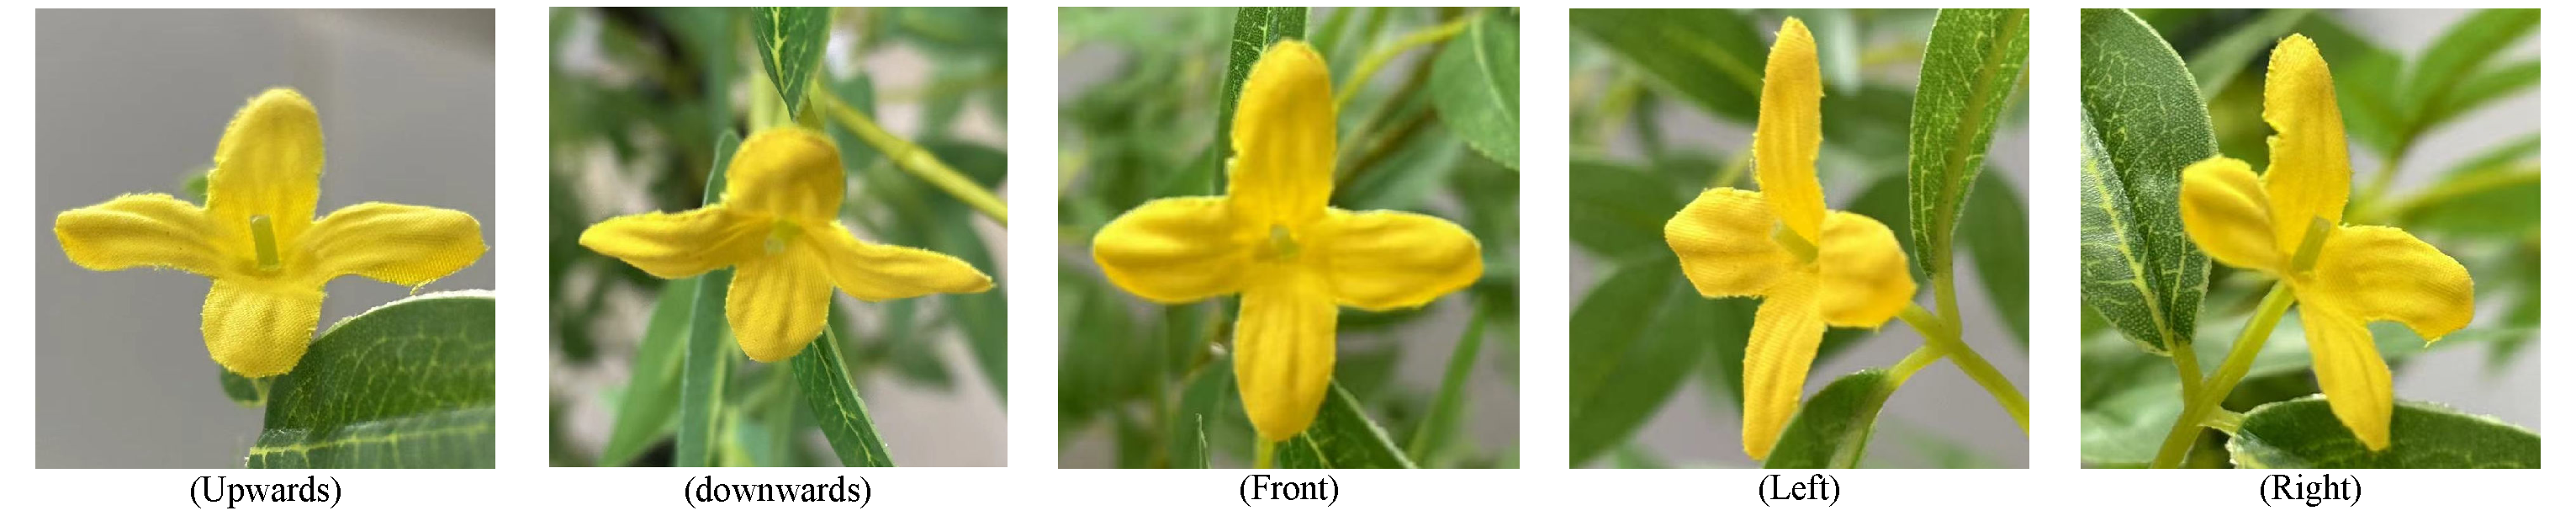
\includegraphics[width=1 \textwidth]{direct_flower}
	\caption[花朵相对于机械臂末端的不同方向姿态示意图]{花朵相对于机械臂末端的不同方向姿态示意图} % 中括号中内容为插图索引中显示内容,可在题注内容过长时使用
	\label{fig:effective_r_1}
\end{figure}
本实验所使用的图像数据均来源于自建授粉图像数据集,数据集中包含了由安装在机械臂上的相机在授粉过程中拍摄的图像,每张图像唯一对应一个待授粉花朵的姿态状态。如\cref{fig:effective_r_1}所示,依据花朵相对于机械臂末端的方向性特征,图像样本被划分为五类:左(L)、右(R)、上(U)、下(D)和正前方(F)。详细的统计信息如表\cref{tab:effective_r_1}所示。




\begin{table}[htbp]
	\centering
	\caption[数据集中不同方向花朵图像的数量统计]{数据集中不同方向花朵图像的数量统计}
	\begin{tabularx}{\textwidth}{YYY}
		\toprule
		\textbf{方向} & \textbf{图像数量} & \textbf{占比(\%)} \\
		\midrule
		L & 261 & 20.6 \\
		R & 274 & 21.7 \\
		F & 230 & 18.2 \\
		U & 256 & 20.3 \\
		D & 243 & 19.2 \\
		\bottomrule
	\end{tabularx}
	\label{tab:effective_r_1}
	
	\vspace{1mm}
	\noindent{\footnotesize 其中 “F”、“L”、“R”、“U” 和 “D” 分别表示前方、左侧、右侧、上方与下方。}
\end{table}


为保证模型输入数据的一致性,首先将机械臂末端相机采集的所有图像统一调整为 $(224 \times 224)$ 的分辨率。随后,对图像进行了归一化处理,将像素值缩放至 $[0, 1]$ 区间,以提升模型训练的稳定性。此外,为增强数据多样性并缓解过拟合问题,应用了包括缩放、裁剪和色彩变换等在内的数据增强策略。

在标签数据方面,假设位置偏差为 $\Delta T = (\Delta T_{x}, \Delta T_{y}, \Delta T_{z})$,旋转偏差为 $\Delta \overrightarrow{W} = (\Delta W_{x}, \Delta W_{y}, \Delta W_{z})$,其中 $||\Delta T|| < D$,$D$ 为常数。根据式~(\ref{eq1}) 和式~(\ref{eq2}) 对平移与旋转误差进行了归一化与缩放处理,使其值域限制在 $[-1, 1]$ 区间内,处理过程如下:

\begin{equation}
	\label{eq1}
	\Delta T_{n} = \frac{\Delta T}{D}
\end{equation}
\begin{equation}
	\label{eq2}
	\overrightarrow{W} = \theta\overrightarrow{V}
\end{equation}
\begin{equation}
	\label{eq3}
	\theta = \sqrt{\Delta W_{x}^{2} + \Delta W_{y}^{2} + \Delta W_{z}^{2}}
\end{equation}
\begin{equation}
	\label{eq4}
	\overrightarrow{V} = \left(\frac{\Delta W_{x}}{\theta},\frac{\Delta W_{y}}{\theta},\frac{\Delta W_{z}}{\theta}\right)
\end{equation}

符号 $\theta$ 在公式\cref{eq3} 中表示旋转角度,$\overrightarrow{V}$ 表示旋转轴方向的单位向量。归一化后的标签数据为 $(\Delta T_{n}, \overrightarrow{V}, \frac{\theta}{2\pi})$。



\subsection{训练细节}

本模型的训练在配备 NVIDIA V100 GPU 的计算环境中进行。优化器采用 Adam 方法,初始学习率设置为 0.01,并使用学习率衰减策略,随着训练过程的推进,学习率逐步降低至 0.00001。训练过程中采用自定义的损失函数(见公式~(\ref{eq7}))。在训练中,损失函数中的超参数 $\alpha$ 与 $\beta$ 会显著影响模型的收敛性能。经过多轮实验验证,最终选定 $\alpha = 0.0025$,$\beta = 1$,该设置有助于模型更稳定地收敛。

在数据划分方面,所有具有不同方向姿态的花朵图像被随机打乱后划分为10个子集,并采用K折交叉验证的方式进行训练。每轮训练选择其中一个子集作为测试集,其余九个作为训练集,总共进行10轮。模型在训练初期收敛迅速,后期趋于稳定。\cref{fig:effective_r_3} 展示了训练过程中损失值、平移误差($TE$)以及旋转误差($RE$)的变化趋势。

\begin{figure}[htb]
	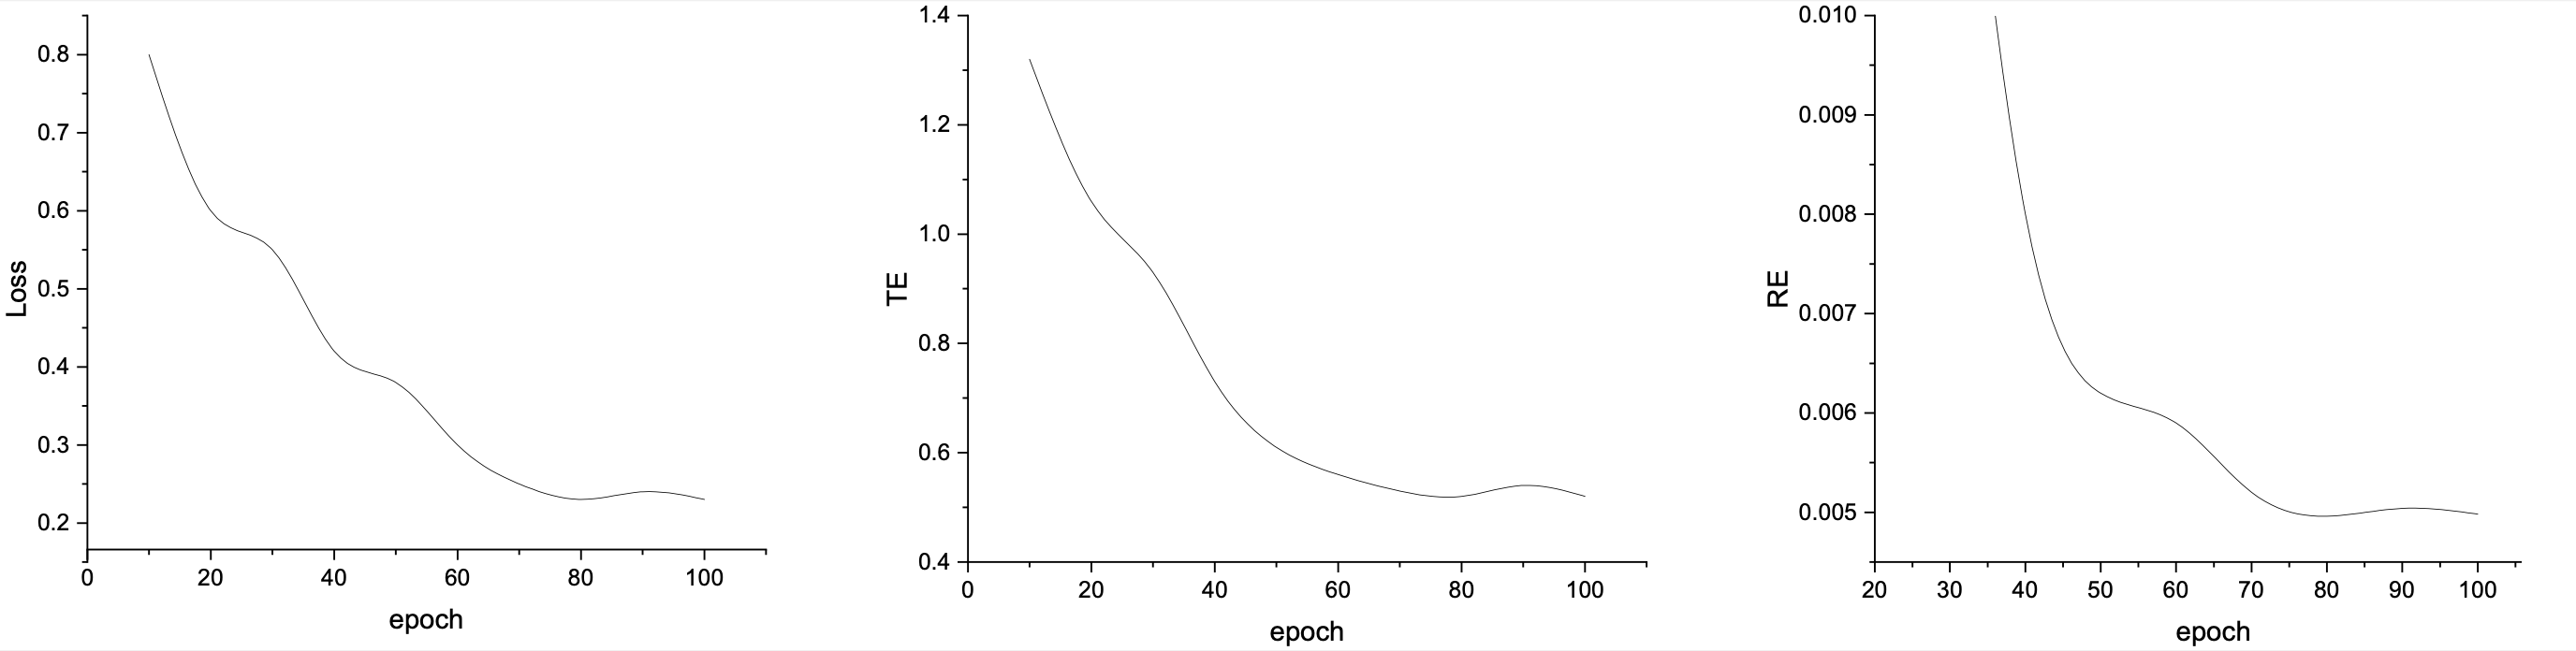
\includegraphics[width=1 \textwidth]{train.png}
	\caption[模型训练过程中的变化曲线]{模型训练过程中损失值(Loss)、平移误差($TE$)与旋转误差($RE$)的变化曲线} % 中括号中内容为插图索引中显示内容,可在题注内容过长时使用
	\label{fig:effective_r_3}
\end{figure}




\subsection{实验结果与分析}

本节重点比较本章所提出方法与没有引入本章所提出方法在机器人末端授粉准确性上的差异,特别是在授粉机器人末端执行器精度与单花授粉效率方面的改进。

我们针对不同方向姿态的花朵进行了分组实验,评估模型的平移与旋转偏差预测精度及检测速度。实验结果表明,不同方向的花朵在预测效果上存在轻微差异。如\cref{tab:effective_r_3} 和\cref{fig:effective_r_4} 所示,朝前方向的花朵具有最小的平移与旋转误差,表现最佳,其次为朝上方向;左右方向由于环境对称性,预测误差几乎一致;而朝下方向的误差最大。但无论方向如何,模型的检测速度(FPS)基本保持稳定。




\begin{table}[htbp]
	\centering
	\caption[模型在不同方向上花朵的实验结果]{模型在不同方向上花朵的实验结果}
	\begin{tabularx}{\textwidth}{YYYY}
		\toprule
		\textbf{方向} & \textbf{平移误差 TE} & \textbf{旋转误差 RE} & \textbf{检测速度 FPS} \\
		\midrule
		L & 0.82 & 0.0049 & 41 \\
		R & 0.82 & 0.0049 & 42 \\
		F & 0.78 & 0.0047 & 43 \\
		U & 0.80 & 0.0048 & 42 \\
		D & 0.87 & 0.0051 & 41 \\
		\bottomrule
	\end{tabularx}
	\label{tab:effective_r_3}
	\noindent{\footnotesize{方向 “F”、 “L”、 “R”、 “U” 和 “D” 分别表示前方、左侧、右侧、上方与下方。}}
\end{table}

\begin{figure}[htb]
	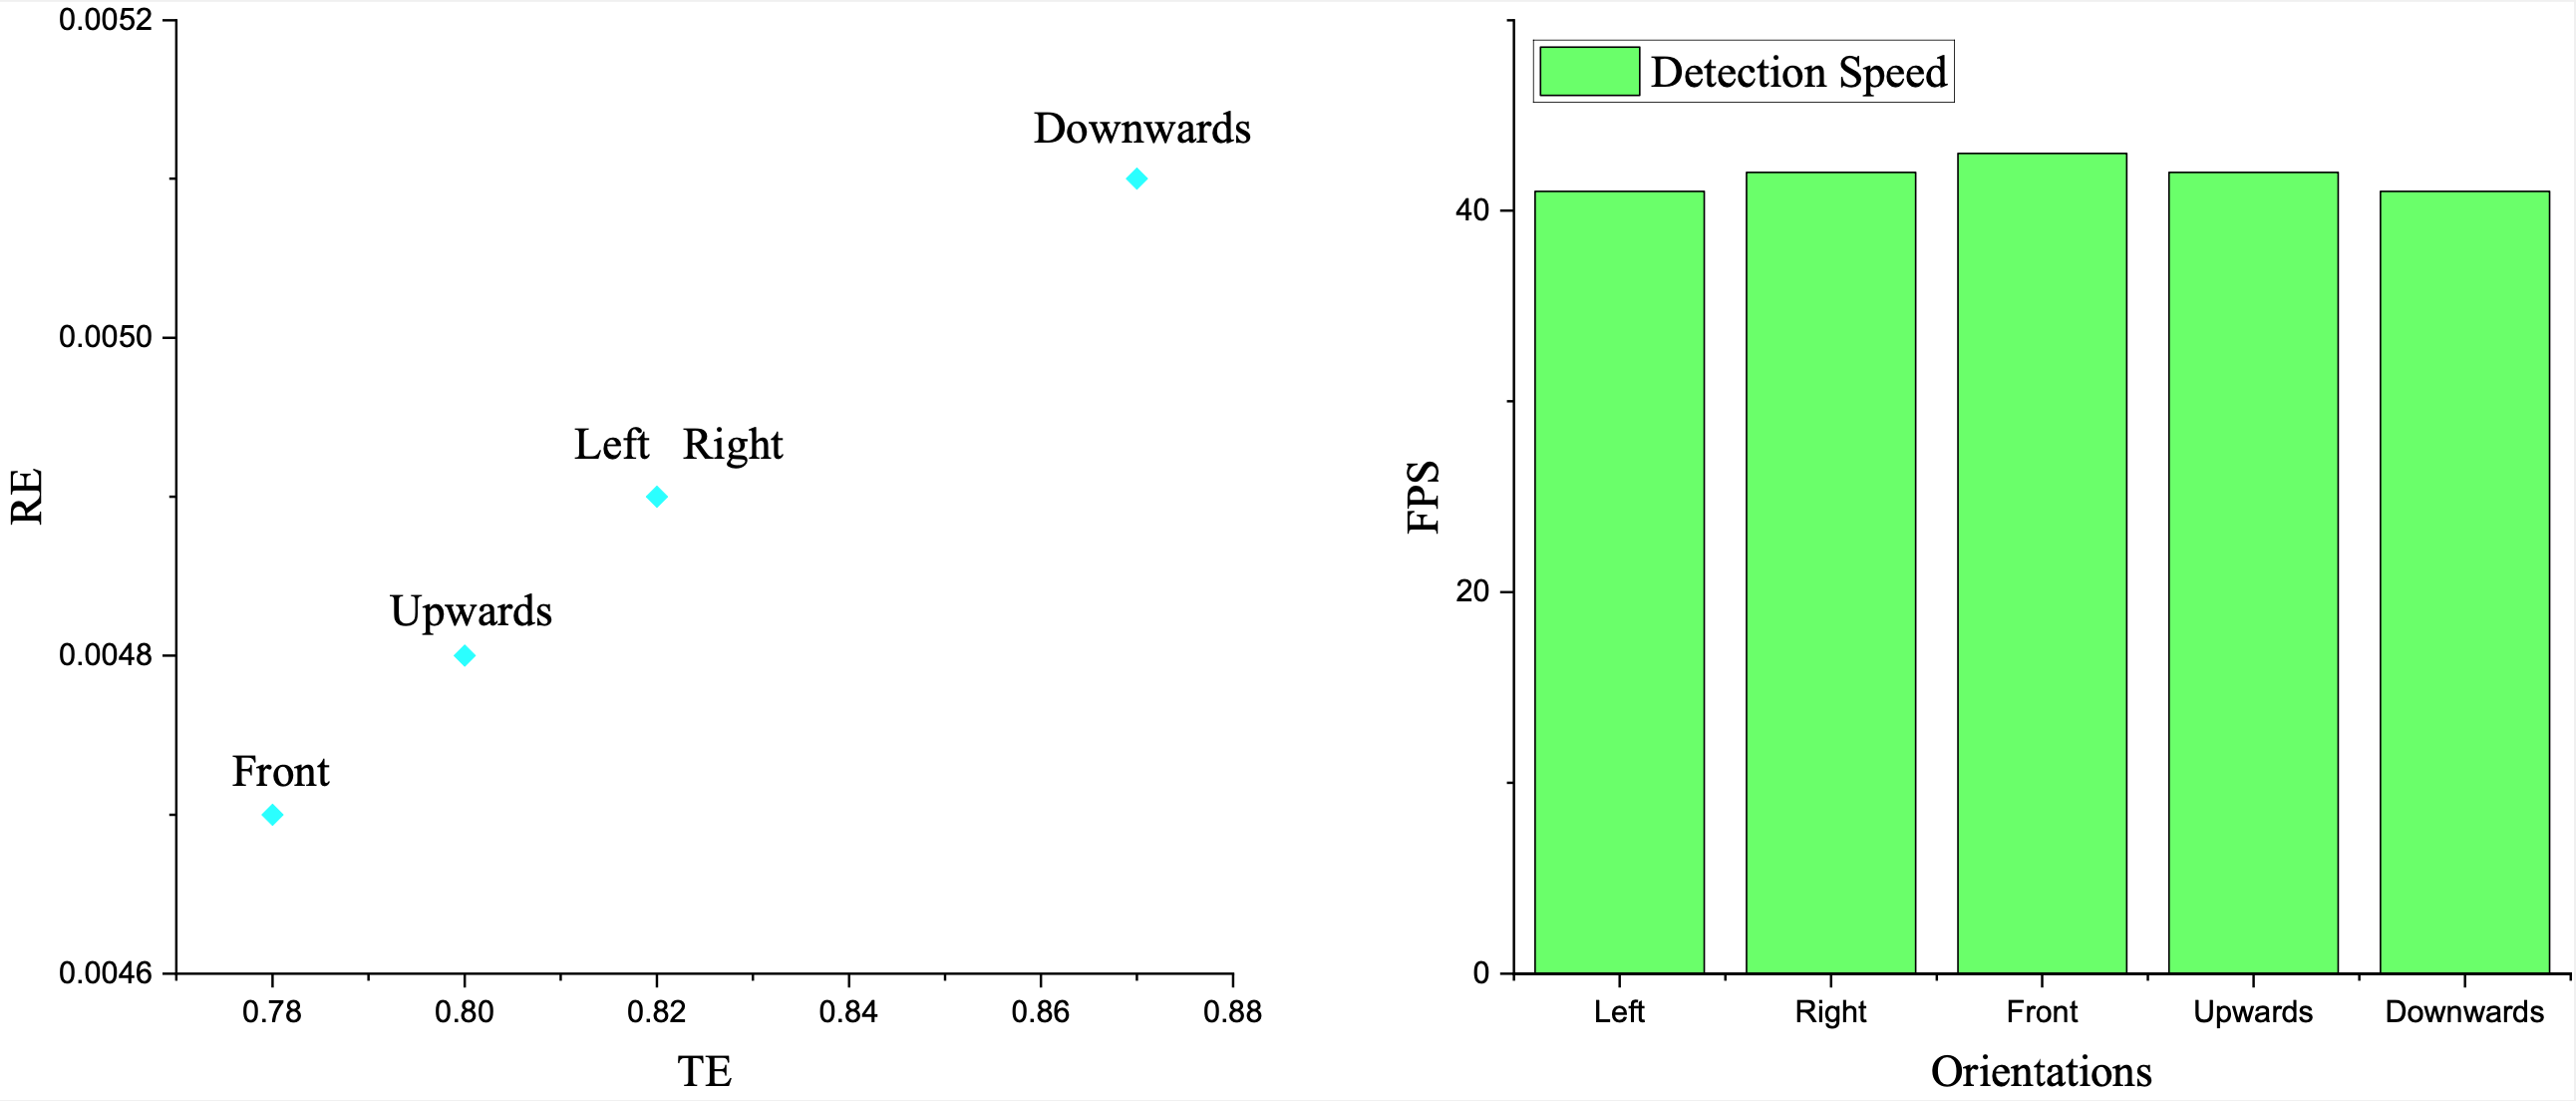
\includegraphics[width=1 \textwidth]{direct.png}
	\caption[模型在不同方向花朵上预测的平移和旋转误差]{模型在不同方向花朵上预测的平移和旋转误差} % 中括号中内容为插图索引中显示内容,可在题注内容过长时使用
	\label{fig:effective_r_4}
\end{figure}

本实验使用前述授粉机器人作为实验平台。机器人完成一次授粉共包含五个步骤,在第四步后其末端执行器相对目标柱头的定位误差为 1.5 cm。在此基础上,我们新增了“精调定位”步骤,输入图像至训练好的模型中,预测平移与旋转偏差,并对授粉末端姿态进行调整。

如\cref{tab:effective_r_4} 所示,加入该“精调定位”步骤后,授粉末端与目标之间的误差显著缩小,为后续伺服授粉步骤减少了搜索范围。实验显示,伺服过程时间从12.7秒缩短至3.1秒,平均成功率达到86.19\%,授粉成功率保持一致。\cref{tab:effective_r_5} 显示我们方法将末端平均定位误差缩小至0.81 cm,精度提升达46.67\%,旋转误差为0.0049,平均单花授粉效率提升达50.9\%。

\begin{table}[htbp]
	\centering
	\caption[本方法引入前后授粉系统各步骤平均耗时比较]{本方法引入前后授粉系统各步骤平均耗时比较}
	\begin{tabularx}{\textwidth}{YYY}
		\toprule
		\textbf{步骤}	& \textbf{baseline 耗时(秒)}	& \textbf{本方法耗时(秒)}     \\
		\midrule
		花朵检测	& 0.0928			& 0.0927		\\
		柱头识别   & 0.025			& 0.024			\\
		位置计算(含运动)    & 1.8			& 1.8			\\
		接近花朵(含运动)   & 4.2			& 4.2			\\
		\textcolor{red}{精调定位}   & /			& 0.024			\\
		伺服授粉(含运动)   & 12.7			& \textcolor{red}{3.1}			\\
		\bottomrule
	\end{tabularx}
	\label{tab:effective_r_4}
	
	\noindent{\footnotesize{“精调定位"步骤是一个额外步骤。增加这一步骤,“伺服”步骤所花费的时间就会大大减少,只需 3.1 秒就能达到相同的授粉成功率。}}
\end{table}
\begin{table}[H]
	\centering
	\caption[本方法与对照方法在不同方向花朵上的误差与耗时对比]{本方法与对照方法在不同方向花朵上的误差与耗时对比}
	\begin{tabularx}{\textwidth}{YYYYY}
		\toprule
		\textbf{方向}	& \textbf{方法}	& \textbf{TE}     & \textbf{RE} & \textbf{耗时(秒)}\\
		\midrule
		\multirow{2}{*}{L}	& baseline			& 1.53			& / & 18.78\\
		& 本方法			& 0.82			& 0.0050 & 9.22\\
		\midrule
		\multirow{2}{*}{R}    & baseline			& 1.52			& / & 18.80\\
		& 本方法			& 0.82			& 0.0050 & 9.23\\
		\midrule
		\multirow{2}{*}{F}    & baseline			& 1.48			& / & 18.85\\
		& 本方法			& 0.80			& 0.0048 & 9.22\\
		\midrule
		\multirow{2}{*}{U}   & baseline			& 1.53			& / & 18.79\\
		& 本方法			& 0.81			& 0.0049 & 9.24\\
		\midrule
		\multirow{2}{*}{D}   & baseline			& 1.55			& / & 18.83\\
		& 本方法			& 0.83			& 0.0052 & 9.26\\
		\bottomrule
	\end{tabularx}
	\label{tab:effective_r_5}
	\noindent{\footnotesize{方向“F”、“L”、“R”、“U”与“D”分别代表前、左、右、上与下。没有引入本章方法的授粉机器人为对照方法。}}
\end{table}
\subsection{消融实验}
\begin{table}[htbp]
	\centering
	\caption[不同主干网络结构与位置编码对模型预测平移与旋转误差精度的影响]{不同主干网络结构与位置编码对模型预测平移与旋转误差精度的影响}
	\begin{tabularx}{\textwidth}{YYYY}
		\toprule
		\textbf{主干网络} & \textbf{位置编码} & \textbf{TE(cm)} & \textbf{RE} \\
		\midrule
		\multirow{2}{*}{ResNet50} & \ding{51} & 0.81 & 0.0049 \\
		& \ding{55} & 1.19 & 0.0051 \\
		\midrule
		\multirow{2}{*}{ResNet18} & \ding{51} & 0.92 & 0.0053 \\
		& \ding{55} & 1.33 & 0.0054 \\
		\midrule
		\multirow{2}{*}{ResNet101} & \ding{51} & 0.86 & 0.0050 \\
		& \ding{55} & 1.21 & 0.0050 \\
		\midrule
		\multirow{2}{*}{VGG16} & \ding{51} & 0.96 & 0.0053 \\
		& \ding{55} & 1.32 & 0.0055 \\
		\midrule
		\multirow{2}{*}{VGG19} & \ding{51} & 0.99 & 0.0054 \\
		& \ding{55} & 1.33 & 0.0055 \\
		\midrule
		\multirow{2}{*}{DenseNet-121} & \ding{51} & 0.92 & 0.0054 \\
		& \ding{55} & 1.23 & 0.0055 \\
		\midrule
		\multirow{2}{*}{DenseNet-201} & \ding{51} & 1.10 & 0.0055 \\
		& \ding{55} & 1.38 & 0.0057 \\
		\bottomrule
	\end{tabularx}
	\label{tab:effective_r_6}
	\noindent{\footnotesize{表中 \ding{51} 表示该模型使用了位置编码,\ding{55} 表示未使用位置编码。}}
\end{table}
\begin{figure}[H]
	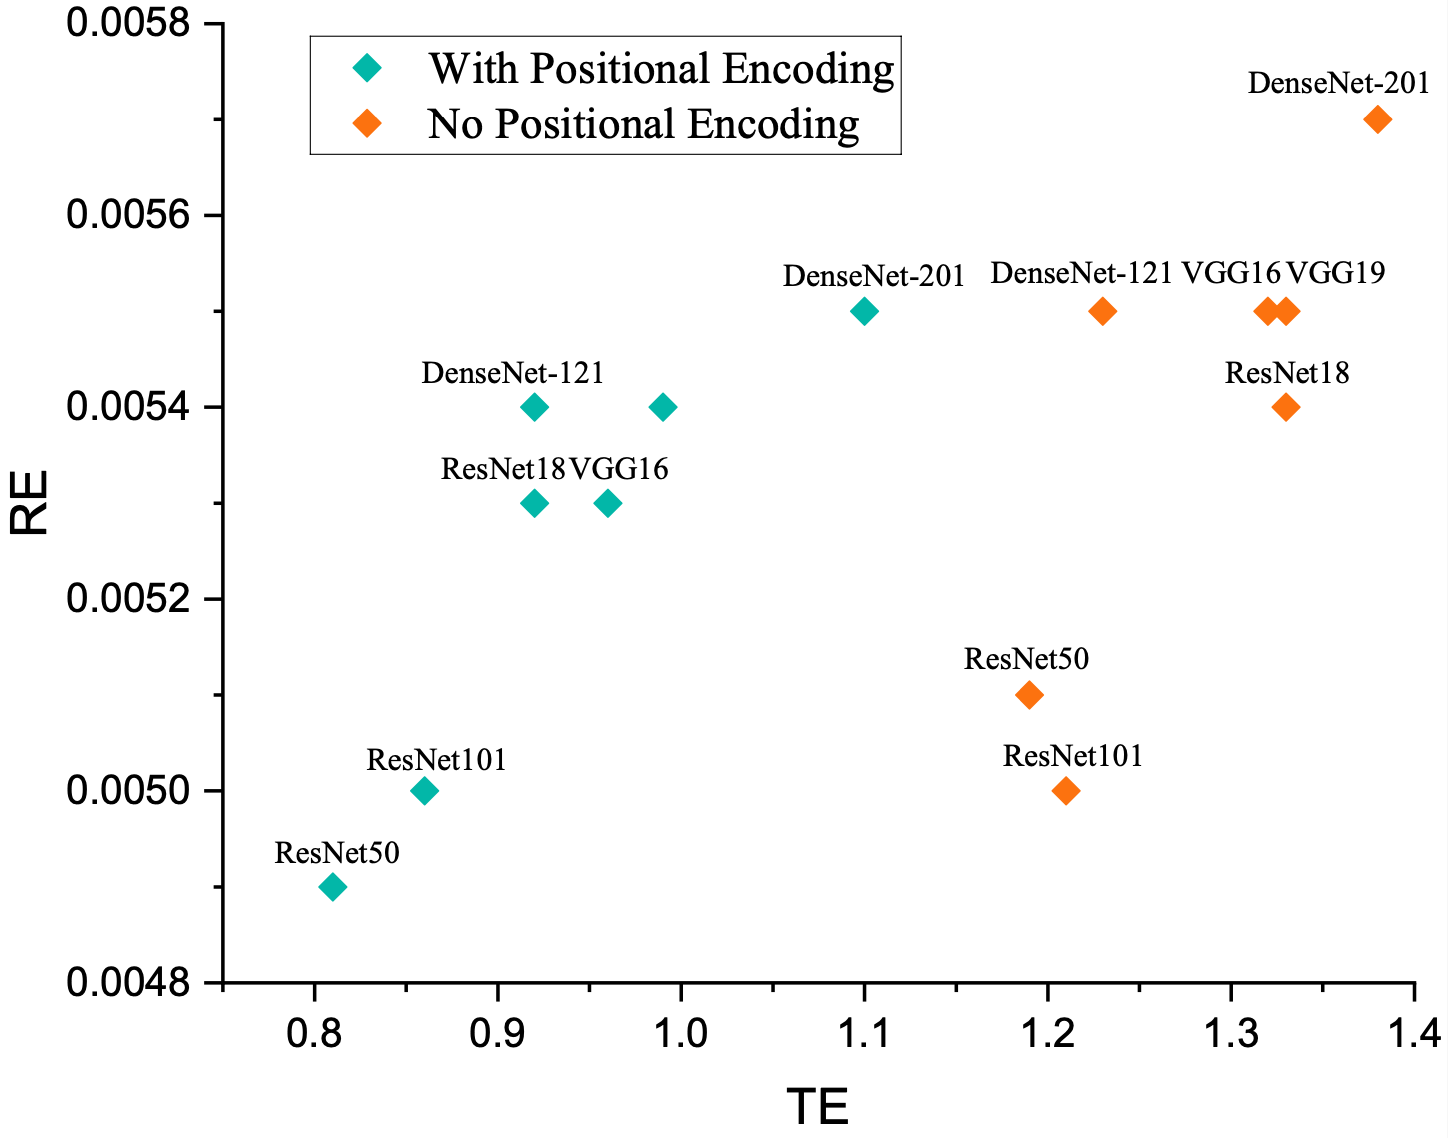
\includegraphics[width=0.6 \textwidth]{result.png}
	\caption[不同主干网络在是否加入位置编码条件下的平移误差]{不同主干网络在是否加入位置编码条件下的平移误差} % 中括号中内容为插图索引中显示内容,可在题注内容过长时使用
	\label{fig:effective_r_5}
\end{figure}
本研究开展了多组消融实验,以验证不同主干网络结构(Backbone)及位置编码的引入对模型平移偏差误差与旋转姿态偏差误差预测精度的影响。我们选取 ResNet50、ResNet18、ResNet101、VGG16、VGG19\cite{simonyan2014very}、DenseNet-121 与 DenseNet-201\cite{huang2017densely} 作为特征提取主干网络,并在每个主干结构下分别进行了添加与不添加位置编码的对比实验。

实验结果如\cref{tab:effective_r_6} 和\cref{fig:effective_r_5}所示,主干网络结构的选择及是否引入位置编码对模型的最终预测精度具有显著影响。其中,采用 ResNet50 作为主干网络并引入位置编码的模型在平移偏差与旋转姿态偏差预测中表现最优,分别达到 0.81 cm 与 0.0049 的误差。



\section{本章小节}

本章提出了一种基于 Transformer 的方法,实现了仅依赖 RGB 图像信息,对授粉机器人末端与目标授粉位置之间的平移误差与旋转姿态误差的端到端预测。实验结果表明,该方法能够有效地将末端执行器的定位误差控制在一定范围内,从而提升了整体的授粉作业效率。

在实验过程中,我们发现所提出的方法在面对不同方向的花朵时预测结果存在轻微差异,尤其是在处理朝下方向的花朵时,平移与旋转误差略有增大。这可能与机器人相机的观察角度相对于花朵方向的关系有关,使得特定姿态下的花朵识别与定位更困难。此外,实验还表明,引入位置编码的模型版本在平移与旋转误差预测方面表现更优,不同主干网络的特征提取能力也对模型性能具有显著影响。

尽管本方法在提升定位精度方面表现出良好的效果,但仍存在一些局限性:(1)本研究所使用的数据集为特定实验环境下采集,模型在多样化环境及不同种类花朵上的泛化能力仍需进一步验证;(2)在光照条件变化较大或存在遮挡的实际农田环境中,模型的鲁棒性可能受到一定影响,从而降低其预测性能。

上述问题提示我们,在未来的研究中仍需进一步优化模型结构与训练策略,以提升其在复杂农业场景中的适应性与可靠性,为实际部署提供坚实基础。




                                              % 可根据需求自行添加章节数

    % !Mode:: "TeX:UTF-8"

\chapter{全文总结与展望}\label{ch:7}

\section{论文工作总结}
本论文围绕“手眼协同的机械臂精准授粉技术”开展研究,针对当前农业场景中存在的花朵识别困难、位姿估计不准、机械臂顺柔控、末端精度不高等问题,提出了一套集视觉感知、位姿重建、柔顺控制与精度补偿于一体的精准授粉解决方案。系统以“感知—定位—控制—评估”闭环思想为指导,完成从花朵检测到末端执行器控制的全流程研究,具有较强的系统性与实用性。

本文的主要工作内容可以概括为下列四个方面:

(1)在视觉感知方面,本文设计了面向复杂农业环境的花朵目标分割方法,结合Mask-RCNN与YOLACT网络,在自建数据集上进行训练,提升了系统在强光、遮挡等条件下的分割精度与实时性。

(2)提出基于对称空间的位姿重建方法,通过深度去噪、三维坐标计算与手眼标定等步骤,实现了高精度的花朵空间定位,为后续柔顺控制提供了可靠基础。

(3)在控制策略设计方面,论文构建了一种两阶段伺服控制框架,结合三次样条插值生成关节空间轨迹,提升了机械臂在连续授粉任务中的运动柔顺性与安全性。

(4)考虑到末端精度对授粉效果的直接影响,本文引入基于Transformer的误差预测网络,通过学习末端的平移与旋转误差,进一步提升了授粉的效率和系统鲁棒性。
\section{后续工作展望}
尽管本研究已在精准授粉任务中取得了较为有效的成果,但仍存在一些值得进一步研究与改进的方向:

(1)复杂环境下的视觉感知鲁棒性仍需提升。当前模型在极端光照条件、严重遮挡情况下的分割与位姿估计精度仍有下降趋势,未来可考虑引入多模态感知技术(如RGB-IR或多光谱)与时序信息增强网络,提高系统在动态环境中的适应能力。

(2)控制系统的泛化能力有待加强。目前的控制策略主要针对番茄花朵设计,缺乏对其他作物品种的适应能力。未来研究可从模型迁移、任务参数化等方向出发,实现系统对多品种、多任务场景的通用控制。

(3)末端误差补偿机制尚未形成闭环反馈。当前Transformer网络基于前馈预测实现误差修正,未来可结合视觉伺服与力觉传感反馈,构建具备自适应与自校准能力的误差闭环补偿系统,进一步提高授粉精度。

(4)系统集成与移动作业能力仍有限。当前实验平台部署于静态环境中,后续可基于SLAM与路径规划算法,实现机械臂平台的自主移动授粉功能,朝着全自主、多目标的农业智能作业系统迈进。

综上所述,本文研究为实现农业自动化中的精准授粉提供了可行的技术路径与理论支持,具有良好的应用前景和研究推广价值。未来将在多模态感知、柔顺控制、自主决策与平台集成等方面持续深入探索,助力智能农业机器人技术的发展与落地应用。                                            % 总结与展望
    
% ------------------------------------------------------------------------------------------

    \ThesisBibliography                                                    % 参考文献
    \ThesisAcknowledgement                                                 % 致谢
    \ThesisAchievement                                                     % 攻读专业硕士学位期间取得的成果

% ------------------------------------------------------------------------------------------    
\end{document} 
